\documentclass{article}
\usepackage[margin=1.5in]{geometry}
\usepackage{amsmath}
\usepackage{lipsum}
\usepackage{caption}
\usepackage{float}
\usepackage{subfig}
\usepackage{graphicx}
\usepackage[utf8]{inputenc}
\usepackage{nameref}
\usepackage{pgfplots}
\usepackage{siunitx}
\usepackage{tikz}
\usepackage{amsmath}
\usepackage{color}   %May be necessary if you want to color links
\usepackage{hyperref}
\hypersetup{
    colorlinks=true,
    linktoc=all,     %set to all if you want both sections and subsections linked
    linkcolor=blue,  %choose some color if you want links to stand out
    citecolor=black,
    filecolor=black,
    linkcolor=black,
    urlcolor=cyan,
}

\newcommand{\Newnameref}[1]{\textit{\nameref{#1}}}
\pgfplotsset{compat=1.13}
\DeclareMathOperator*{\argmax}{arg\,max}
\DeclareMathOperator*{\argmin}{arg\,min}

\begin{document}


\thispagestyle{empty}
\title{
\huge{\textbf{Localization for FRC}} \\
\vspace{1.0cm}
\small{A Major Qualifying Project Report} \\
\vspace{0.7cm}
\small{Submitted to the Faculty of the} \\
\vspace{0.7cm}
\large{WORCESTER POLYTECHNIC INSTITUTE} \\
\vspace{0.7cm}
\small{In partial fulfillment of the requirements for the} \\
\vspace{0.7cm}
Degree of Bachelor of Science in \\
\vspace{0.7cm}
\large{Robotics Engineering and Computer Science} \\
\vspace{0.7cm}
\small{by}}
\author{Jinan (Dorothy) Hu, Peter Mitrano, Kacper Puczydlowski, Nicolette Vere}

\maketitle{}

\newpage


\section*{Abstract}

  We present research, design, analysis, and implementation of a low cost localization system for high speed, cluttered, multi-robot, environments. In these environments, no individual sensor is sufficient for accurate localization. We use the FIRST Robotics Competition as a motiving example. We survey localization techniques application as a whole, and subsequently identify which of these techniques are most applicable. We define criteria for successful localization in these environments, then describe experimental results to characterize and benchmark individual sensors and algorithms. Furthermore, we describe the datasets we have collected and released, and finally, we provide a description of how we combined a subset of the proposed techniques in a complete localization system.




\section{Introduction}

  \subsection{Motivation}

    Imagine you arrive for the first time to spectate an FRC competition. The robots are placed carefully around the field, the announcer counts down to the beginning of the autonomous portion of the match, and you wait in anticipation for these great machines to come to life. The buzzer blares, and nothing moves. Unfortunately, this is a fairly common occurrence, and even more commonly the robots will simply drive roughly forward for a few seconds before stopping and waiting for the teleoperated portion of the match to begin. In many cases, interesting autonomous behavior requires knowing the position of the robot. In order to pick up game pieces or interact with elements of the field, it is incredibly useful to know the position and orientation of the robots. This is the motivation for our MQP. We take the first steps towards a principled and robust solution to this problem. FRC is just one example of a high-speed, cluttered, multi-robot environment, and while there are tried-and-true solutions to many instances of the general localization problem, these FRC like environments currently lack an accurate and inexpensive solution. FRC is a challenging environment because the robots make rapid and aggressive maneuvers by human drivers for part of the time, and at other times are under complete autonomy. Another challenge is that FRC fields are cluttered with other robots and game pieces such as soccer balls, pool noddles, or inflatable shapes, and these objects change from year to year. A successful localization system for FRC must support up to six robots, and must be robust to occlusion from the playing field elements, unpredictable lighting, and frequent impacts. Our research suggests that there are at least five appropriate methods for localization: cameras and tags, radio and ultrasonic beacons, optical flow, dead reckoning with encoders, and dead reckoning with an IMU. All of these methods have seen success in robot localization, but we will argue that none of them are sufficient on their own.

  \subsection{Problem Statement}

    We desire a system for determining the pose consisting of $x$ and $y$ position and orientation $\theta$ of the robot. At the highest level, the goal is to allow robots to query their absolute pose on the field at any time. This information is a prerequisite for interesting behaviors such as path following, picking up game pieces, and navigating to feeder stations. An important criteria for our system is that it work well not only on the FRC field, but in teams practice spaces. This means we cannot rely on an \textit{a priori} map of the geometry of the environment, or any other knowledge of the lighting, sound, and surface conditions.

  \subsection{FIRST Robotics Competition} \label{section:frc}

    The FIRST Robotics Competition is an international high school aged robotics competition:
    \begin{quotation}
      ``Under strict rules, limited resources, and an intense six-week time limit, teams of students are challenged to raise funds, design a team brand, hone teamwork skills, and build and program industrial-size robots to play a difficult field game against like-minded competitors.'' \cite{kamen_first_2015}.
    \end{quotation}

    Each year, a new game is designed for the teams to tackle. However, the field remains a constant size of 54'3" long by 26'3" wide. This field can contain walls, ramps, towers, or any other number of obstacles from year to year. A rendering of the 2018 field is shown in Figure \ref{fig:frc_field}. Furthermore, the field usually contains small balls or other game pieces that the robots must manipulate. In preparation for these competitions, teams will often build mock field elements or game pieces to practice with in their shops. These practice spaces vary tremendously in size and in terms of how the team can operate in the space (see \ref{appendix:survey}, \ref{section:defining_success}). The robots built for these competitions are typically several feet in every direction, with differential or Mecanum drive, and can usually drive up to \SI{4}{\meter\per\second}. Each match begins with a brief 15 second autonomous period, and continues with roughly 2 minutes of teleoperated control.

    \begin{figure}[H]
      \centering
      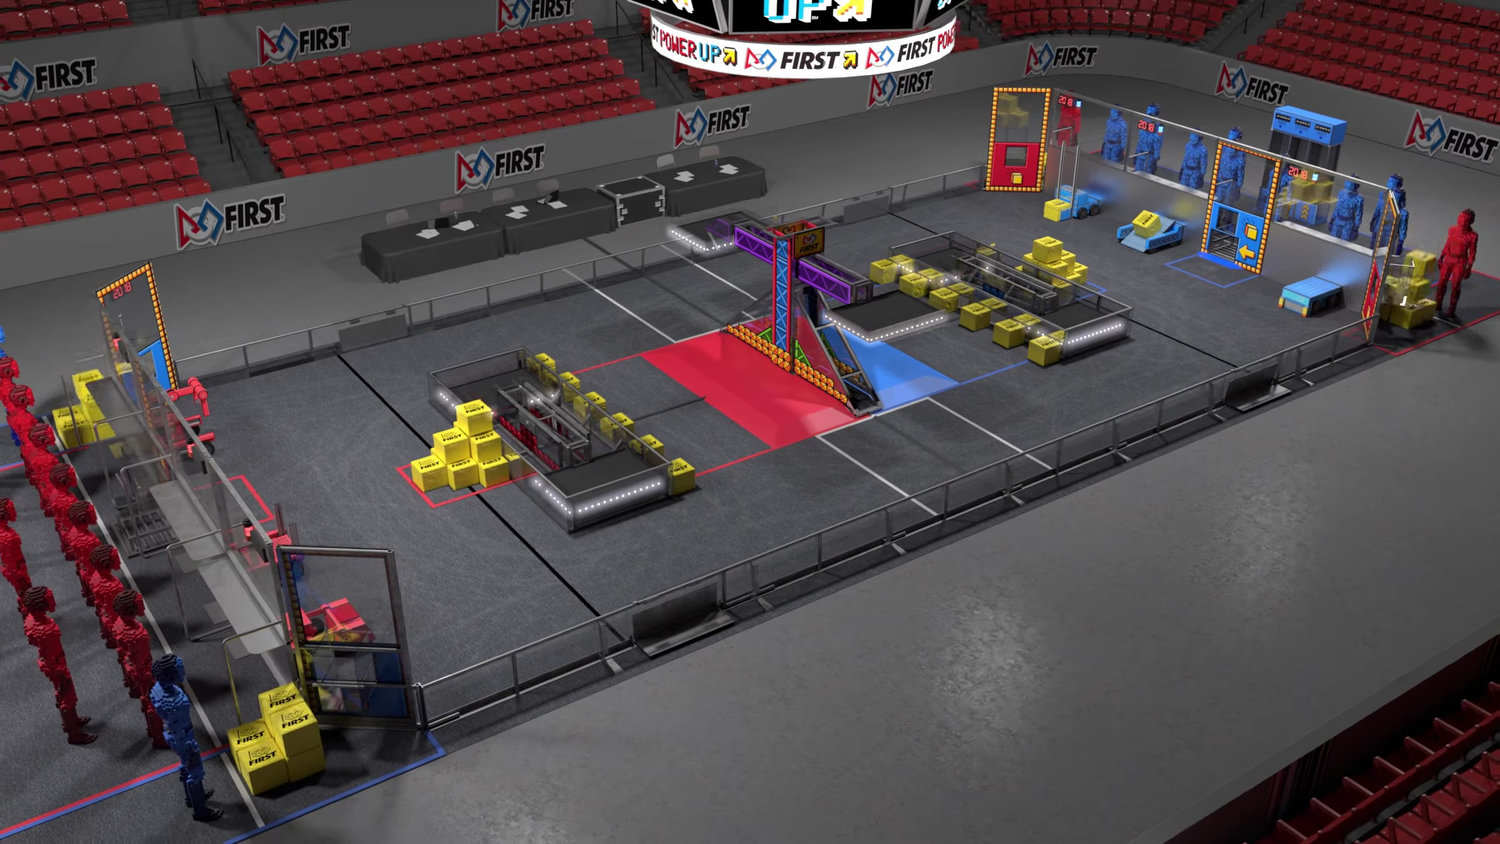
\includegraphics[width=0.75\linewidth]{./images/FIRST_2018_field.jpg}
      \caption{the FIRST Robotics 2018 Competition Field}
      \label{fig:frc_field}
    \end{figure}

    The robots themselves contain a range of sensors, but the sensors useful for localization commonly include encoders on the drive wheels, an IMU, and a camera. Presently, teams use often a provided API to compute the current angle from the IMU, and may use encoders to measure the forward distance traveled. Teams often use the camera to detect large retro-reflective pieces of tape using simple blob detection with OpenCV in order to align their robots with certain field elements. While some teams use the camera or other sensors to go well above and beyond this, most teams do not have the resources or talent to do so \cite{balaji_zebravision_2017}. Overall, while many robots contains sensors which are useful for localization, very few teams are able to extract a reliable position estimate from these sensors.

  \subsection{Key Contributions}

    The key contributions of this MQP are:
    \begin{itemize}
      \item Survey of localization techniques applicable to FRC-like environments
      \item Set of metrics which define a successful localization system for FRC
      \item Suite of 20+ experiments (see \Newnameref{section:experiments}) spanning many different sensing methods
      \item Dataset of robot sensory readings and associated ground-truth position
      \item And a sample implementation oF a full localization system based on all this knowledge
    \end{itemize}

\tableofcontents




\section{Survey of Localization Techniques} \label{section:related_work}

   In this section we provide an overview of the most common and applicable localization techniques. Overall, the problem of localizing a mobile robot can be viewed as accurately measuring the absolute distance to known landmarks, or by measuring the changes in position over time. All localization methods lie somewhere on a spectrum between these two approaches, and we will henceforth refer to these two ideas as global and local pose estimation. Some of the high level techniques for robot localization are: measuring range at various points around the robot and matching these readings to a map, measuring time of flight or difference of arrival time to calculate distances to known locations, recognizing landmarks and computing pose relative to those landmarks, and measuring changes in pose and accumulating these changes over time. There are different sensors that can be used for each of these techniques, such as laser range finders, cameras, inertial measurement units (IMU), encoders, radio, infrared light, visible light, ultrasonic and audible sound. Although there are a tremendous number of possible methods for indoor mobile robot localization, there are a few which have received the most attention and shown the most success. These include, but are not limited to:
  \begin{itemize}
    \item LIDAR mapping
    \item Ultrasonic mapping
    \item IMU and Encoders fusion
    \item Infrared or Radio and Ultrasonic beacons
    \item Wireless network methods based on signal strength
    \item Cameras with visually identifiable tags
    \item Optical flow mice and cameras
  \end{itemize}

  In our research, we learned how these techniques work and found descriptions and implementations to figure out whether they are appropriate for high-speed, cluttered, multi-robot environments like FRC. These descriptions and implementations are presented in this section with the purpose of demonstrating a thorough literature review and of providing background information to the reader.

  \subsection{LIDAR Mapping}
    LIDAR is a sensor that works by measuring the amount of time it takes a laser to return to the LIDAR after hitting a desired object \cite{keith_lidar_2007}. Since light moves at a constant speed, the LIDAR can calculate the distance between itself and the object that light was hitting. The formula to compute distance is $\frac{d*c}{2}$, where $d$ is the distance to the object, $c$ is the speed of light and the division by two accounts for traveling to the object and back. By repeating this process at different angles the LIDAR can produce a map of its surroundings by finding the distance between it and surrounding objects within its detecting range.

    There are three types of information LIDAR can collect depending on the type of LIDAR. The first is the range to the target which is found using a topographical LIDAR. A differential Absorption LIDAR can find the chemical properties of the targets it is measuring. A Doppler LIDAR can measure the velocity of a target. For our scenario, we concern ourselves only with topographical LIDAR methods.

    Most LIDAR have two main pulse systems for measuring distance. The first system uses a micropulse have lower powered lasers that are usually considered safer \cite{keith_lidar_2007}. The wavelength for these is typically 1.0-\SI{1.5}{\meter} \cite{lidar_uk_how_2017}. The second system uses high energy lasers and is typically only used for atmospheric measurements \cite{keith_lidar_2007}. The wavelength of these is typically 0.5-\SI{0.55}{\meter} \cite{lidar_uk_how_2017}.
    LIDAR localization works by matching landmarks to some known map. Since the distance between it and those landmarks are known, the LIDAR system can be used to determine its own position \cite{schlichting_vehicle_2016}. Another approach is to match point clouds found on the most recent map produced by the LIDAR to point clouds on the prior map. This has advantages because it does not rely on there being distinguishing features in the environment. But it also takes more time to compute the map since it has to compare more points than a feature to feature map \cite{li_extracting_2010}.

    % TODO:
    % need sources for accuracy and sample implementations

  \subsection{Ultrasonic Mapping}

    Ultrasonic mapping (often referred to as sonar) was one of the first techniques used for indoor robot localization, and has been explored deeply since the 1980's. The most common approach is to use multiple emitter-receiver transducers placed around the perimeter of the robot, measure the range at each of those points, then localized to a given map of the environment \cite{drumheller_mobile_1987}. Alternately, some systems use one sensor and rotate it to achieve the same effect \cite{leonard_mobile_1991, drumheller_mobile_1987}. The algorithms for interpreting the measured distances work by first extracting lines, then matching these lines to an existing map using algorithms such as RANSAC. Reported accuracies of the system in \cite{drumheller_mobile_1987} was 1 ft for position, and \ang{10} for angle. In \cite{drumheller_mobile_1987} and \cite{leonard_mobile_1991}, the reported rate of position updates is \SI{1}{\hertz}. Additionally, some methods will explicitly model the uncertainty of the position estimate, or explicitly model the behavior of ultrasonic sensors to ignore unreliable data. A more recent and sophisticated approach to localizing with sonar can be found in \cite{tardos_robust_2002}, in which 24 sonar sensors in conjunction with encoders were used to perform simultaneous localization and mapping. Their experimental results report drifts of \SI{3.9}{\meter} and \ang{21} over the course of \SI{35}{\meter} of travel.

  \subsection{IMUs and Encoders}
    An inertial measurement unit (IMU) is a sensor reporting the forces acting upon an object, the angular rates of change, and surrounding magnetic field. The device typically comprises an accelerometer, gyroscope, and magnetometer which sense the above data respectively. These devices function by detecting Coriolis forces, which are inertial forces acting in the direction of motion relative to a rotating reference frame. These forces are proportional to the magnitude of the acceleration. These forces may be detected by a simple strain gauge mechanism or object vibrating at a known frequency (the rate of change of vibration frequency is detected) \cite{barshan_inertial_2017}. The premise behind position sensing using this device involves integrating the data with respect to time to calculate position and orientation. This approach was first used in aeronautics to estimate projectile attitude, orientation, and position \cite{nasa_kalman_1999}. High cost IMUs have been used historically for defense and transportation systems; the quality of the sensor is high and the data is reliable in these applications. An inertial navigation system (INS) often comprises multiple accelerometers, gyroscopes, and magnetometers to estimate orientation and position. Their performance is increased by referencing, or filtering, one sensor to estimate the error from another. Simple double integration of a filtered system using expensive sensors is often sufficient for position tracking applications like ballistics or missile tracking \cite{barshan_inertial_2017}.

    In cost-sensitive systems, these simple methods are much less accurate because the low-cost electronics have more drift and noise. Because of integration of accelerometer data, the velocity error term grows linearly and position error grows quadratically. This introduces a need for more sophisticated filtering, sensor fusion, and optimization based approaches. Bayesian filters (Kalman Filter, Particle Filter, \dots) are one family of filtering algorithms commonly used with IMUs.

    If the rate at which the position must be updated is lower than the update rate of the data, many values can be processed and used to calculate an approximation within a given time window. This technique is known as preintegration. Instead of filtering the data, preintegration combines many data points into a single trajectory estimate. Then, it transforms the data into the navigation frame, allowing for a smoother approximation of system position. This was beneficial in cases where global position data was unavailable for extended periods of time, and it also decreases computational load of the localization thread \cite{lupton_visual-inertial-aided_2012}. The authors of \cite{lupton_visual-inertial-aided_2012} describe an overall CPU time of about 10ms for data processing and real-time execution, although the system update frequency is unknown. %TODO: any accuracy information?

    Another method for computing position from IMU data is presented in \cite{vadim_indelman_information_2013}. The state estimate and sensors measurements, which include imagery in addition to IMU data, are represented as a factor graph, and an novel algorithm is presented to update these estimates to approximately-optimally estimate the true state. The main benefit of this approach is improved computational complexity over methods like Bundle Adjustment, without requiring linear or approximately-linear sensor models like with Kalman or extended Kalman filters.

    Due to the widespread availability and well understood algorithms for using IMUs to derive position, there exist libraries for IMU based localization already available to FRC team. Frameworks such as Sensor Fusion 2 (SF2) provide students with algorithms that include double integration, latency correction between IMU and camera data, fusion of encoder and IMU data, and keyframe-based state estimation \cite{kauai_labs_inc_video_2017}. These algorithms use known system parameters, such as update frequencies of sensors, frame transformations between sensors, and data from landmarks for filtering and position estimation. Additionally, the data is accurately timestamped and easily accessible to the vision processing thread. This way, the user receives an updated pose estimate without lag and has a history of the orientation. However, we suggest that these libraries are not quite robust enough for FRC teams to rely on them for accurate position (see \nameref{section:defining_success})

  \subsection{Beacon systems and Wireless Networks} \label{section:beacons_background}

    Beacon systems generally use ultrasound and or radio as a medium and either signal strength, phase shift, or time to measure distance to the beacons. Among radio systems, the system in \cite{bahl_radar:_2000} identified the location of people moving around buildings using signal strength in the 2.4gHz band received at three or more beacons, and they report accuracy of a few meters with an update rate of at most four times per second. The systems described in \cite{digiampaolo_mobile_2014} uses passive RFID tags on the ceiling and an RFID transmitter on the robot, and report an accuracy of 4\si{\centi\meter} within a 5\si{\square\meter}. Another RFID system \cite{saab_standalone_2011} also uses signal strength to RFID, and reports accuracies for various configurations ranging from 1\si{\centi\meter} to 3\si{\meter}. These RFID systems use readers that cost over \$500.

    There are also countless localization systems that use standard wireless networks. A comprehensive survey of these systems can be found in \cite{liu_survey_2007}. Systems that use signal strength in standard wireless LAN networks have achieved up to 10\si{\centi\meter} accuracy and hundreds of updates per second. Another radio beacon solution is to substitute single-frequency radio with Ultra-wideband radio. These systems can achieve centimeter level accuracy, but they use obscure or custom made transmitters and receivers that cost in the hundreds of dollars \cite{zebra_dart_2017} \cite{pozyx_pozyx_2017}.

    Among ultrasonic beacon systems, \cite{kleeman_optimal_1992} uses the raw arrival times of ultrasonic pulses over time plus odometry together in a Kalman filter. Many beacon systems use the speed difference between sound and electromagnetic waves to measure system. Systems like \cite{smith_tracking_2004}, \cite{ward_new_1997}, and \cite{kim_advanced_2008} send radio pulses followed by ultrasonic pulses. This is known as the ``Cricket'' style of beacons. Nodes in the network us the difference in arrival time of these two signals to measure distance. Alternately, some systems use infrared pulses in place of radio \cite{ghidary_new_1999} \cite{yucel_development_2012}. These systems are inexpensive, and report accuracy of between \SI{2}{\centi\meter} and \SI{14}{\centi\meter}.

    In the remainder of this paper, we will always be referring to the ``Cricket'' beacon localization method. This method has been shown to be accurate and affordable, and as we will discuss in the \nameref{section:trade_off_analysis} section, it nicely compliments our other proposed methods of localization.

  \subsection{Cameras with Visual Tags}

    Most methods for indoor localization assume some amount of either natural landmarks or artificial landmarks in the environments as references to absolute positions. In either case, the general approach is to calculate the pose of the robot with respect to one or more landmarks, then use the known position of the landmarks to calculate the pose of the robot in a global frame. Another similar approach is using 3D models and 2D to 3D matching techniques. The system described in \cite{sattler_fast_2011} had accurately localized the camera's position using this 2D to 3D mapping technique. The most common method for localization is artificial landmarks. Common artificial landmarks include 1D binary barcode, 2D binary barcode and 2D colored barcode. The system in \cite{lin_localization_2004} used cameras and ID tags on the ceiling, which were \SI{2}{\meter} away from the floor. A web camera facing the ceiling was mounted on a moving robot with a speed of \SI{20}{\centi\meter\per\second}. The result of the experiment in \cite{lin_localization_2004} showed that this method was accurate even though there was an unevenness between the ceiling and the floor. Another system \cite{huh_mobile_2007} also used camera and tags. However, instead of sticking ID tags on the ceiling, it put invisible tags on the floor by every \SI{3.75}{\centi\meter}. The camera it used was surrounded by a UV light, which allowed the camera to capture those invisible tags. This system performed really well in homelike environments, and the authors report only a few centimeters of error. Another barcode based localization system for robots with very limited memory and computational resources (8 KB memory, 16 MIPs) \cite{dias_barcode-based_2012} used 1d barcodes as references. Using a camera with 80 vertical pixels and 640 horizontal pixels, the system achieved localization within \SI{7.8}{\centi\meter} of error on average. Ultimately, cameras with artificial visual markers have been shown to be accurate enough for our application (see section \ref{section:defining_success}) but are highly dependant on the various assumptions about tag placement, camera quality, processor capabilities, and the required frequency of position estimates.

    \subsubsection{ArUco and MarkerMapper}

      ArUco is one implementation of artificial landmark based localization that has been used extensively in robotics research. The ArUco library (\url{https://sourceforge.net/projects/aruco/}) provides a function for estimating the pose of an object by minimizing the squared sums of the distances between the projected points and the measured points (reprojection error). The side length of each tag is known and input into the program. The measured points (two corners, minimally) are used to obtain a point estimate in 3D space. Multiple point estimates from each corner are used to calculate the pose of the ArUco tag's centroid. The projected points are parameterized by the camera matrix, which uses the pinhole camera model. The reprojection error corrects the pose estimate based on the calibrated values. An example of a correctly detected ArUco tag can be seen in Figure \ref{fig:example_aruco_detection}.

      \begin{figure}[H]
        \centering
        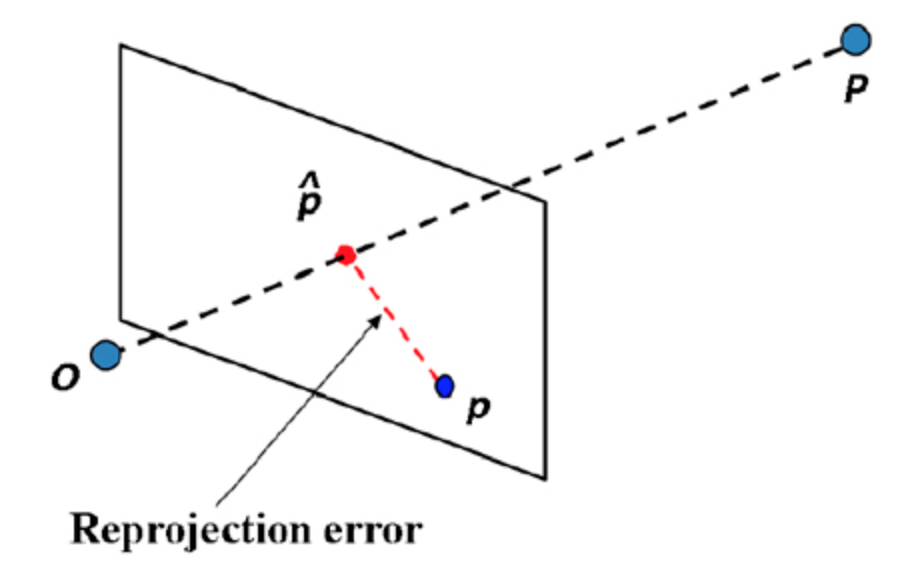
\includegraphics[width=0.5\linewidth]{./images/reprojection_img.png}
        \caption{Calculating reprojection error \cite{richard_hartley_multiple_2003}.}
        \label{fig:reprojection_img}
      \end{figure}

      MarkerMapper (\url{https://sourceforge.net/projects/markermapper/}) builds on top of the detection of individual markers. Markers are first scattered around the environment, then MarkerMapper can be used to build a map of their poses in space. The ID of the origin is input into the program. By estimating the pose of each tag in a camera frame, a map of transforms between tags was developed. Then, the position of the robot's camera, and by extension the robot itself, can be found with respect to detected markers. When the map is complete, the user is able to query the pose from the origin using data from any tag in the workspace. This approach has the advantage of not requiring tags to be placed carefully at known locations, which is a difficult problem in cluttered environments.

      \begin{figure}%
        \centering
        \subfloat[raw data]{{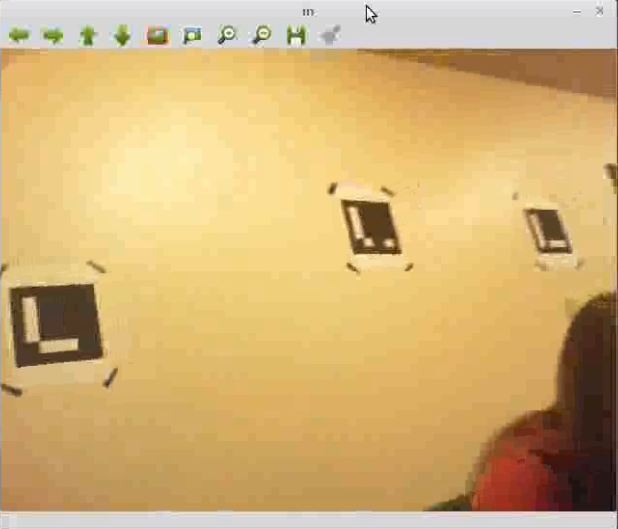
\includegraphics[width=5cm]{./images/aruco_vis2.png} }}%
        \qquad
        \subfloat[annotated frame]{{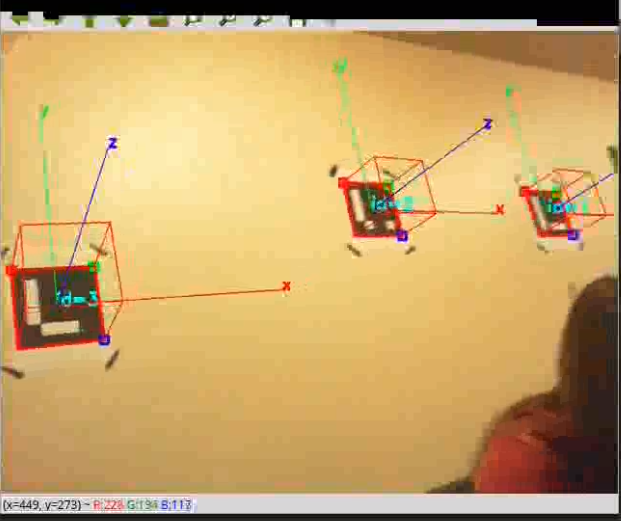
\includegraphics[width=5cm]{./images/aruco_vis1.png} }}%
        \caption{Visualization of pose estimate}%
        \label{fig:example_aruco_detection}%
      \end{figure}

      % TODO: add accuracy and other metric information from existing work using ArUco and MarkerMapper

  \subsection{Optical Flow}

    Optical flow is the ability to track changes between cameras frames and measure the differences between them to track position. In other words, optical flow is a collection of techniques for finding the movement of objects between images or video frames. More precisely, optical flow looks at the movement of pixels among images. There are many assumptions about the image that has to be made in order to apply optical flow. The first is that the lighting in the image stays consistent throughout the sequence of images. Images with inconsistent lighting or transparent objects would violate this assumption. Limiting the amount of inconsistencies in each sequence of images leads to more accurate optical flow. % FIXME: citation?

    There are many methods of calculating optical flow that deal with different constraints. This first is the Horn and Schunk method which calculates optical flow looking at all pixels in an image. Methods which consider all the pixels are called global methods. Along with the lighting constraint it also adds that the image should be as smooth as possible and have few variations in its coloration. The closer the amount of variations is to zero the more accurate the optical calculation will be\cite{odonovan_optical_2005}.

    The optical flow vector for each pixel is calculated using the equation below. $I_x$  and $I_y$  are the spatial gradient of the current pixel. Spatial gradient refers to the path the pixel is moving along. $I_t$ is the temporal gradient of the current pixel. Temporal gradient is how similar the motion of the pixel is to its neighbors \cite{sun_optical_2008}. $\alpha$ is a weighting term. $\bar{u}$ and $\bar{v}$ are the components of the average optical flow vector of neighboring pixels. The equation is shown below \ref{eq:hotnandschunk} \cite{odonovan_optical_2005}. $n$ represents which iteration the optical flow calculation is on. Each current pixels' optical flow is calculated based on the optical flow of the pixels at the previous iteration. Optical flow calculation will iterate from pixel to pixel until it has calculated optical flow for each pixel.

    \begin{equation} \label{eq:hotnandschunk}
      \begin{split}
        u^{n+1} &= \bar{u}^n-\frac{I_x[I_x\bar{u}^n+I_y\bar{v}^n+I_t]}{\alpha^2+I_x^2+I_y^2} \\
        v^{n+1} &= \bar{v}^n-\frac{I_x[I_y\bar{u}^n+I_y\bar{v}^n+I_t]}{\alpha^2+I_x^2+I_y^2}
      \end{split}
    \end{equation}

    Optical flow can also be done locally using the Lucas Kanade method \cite{sun_optical_2008}. This method is based on the assumption that the optical flow vector of pixels are similar to their surrounding pixels. This method finds optical flow vectors that are consistent with its neighboring pixels' temporal gradients and spatial gradients. Each neighbor is then given a weight based off of how close it is to the pixel. The farther away a pixel is, the lower a weight it is assigned. This is because spatial and temporal gradients are based on how far away a pixel is so the error will be larger. Having a lower weight will reduce the error. The formula for the optical flow vector is a least squares equation shown below in equation \ref{eq:lucaskanade} \cite{odonovan_optical_2005}.

    \begin{equation} \label{eq:lucaskanade}
      \begin{split}
        E_v &= \sum_{p\in\Omega}W^2(p)[\nabla I(p)\cdot v + I_t(p)] \\
      \end{split}
    \end{equation}

    $\nabla I(p)$ and $I_t(p)$ are the spatial gradient and the temporal gradient for each of the neighboring pixels $p$. $v$ is the optical flow vector for pixel located at $(x, y)$ on the image. $W(p)$ is the weight assigned for each pixel. Local methods tend to work better since they do not allow information about vectors to spread to unrelated regions of the image. This issue of information spreading to unrelated areas of the image is especially problematic in global methods when the assumptions about consistent smoothness and illumination are not fully met. There are a variety of other optical flow methods that focus on different ways of comparing pixels within images but local and global are the most popular methods \cite{odonovan_optical_2005}.

    Optical flow has been used for multi-sensor localization in indoor, feature-rich environments \cite{gao_qingji_onboard_2015}. This method is also sometimes called visual odometry. In this work, the authors use a PX4FLOW optical flow sensor to capture 64x64 pixel images at 100 FPS, and an ultrasonic range sensor to measure distance from the ground. The data from the camera was used to obtain a velocity information using optical flow and a position estimate using landmark detection on the images. These were fused with attitude data from an onboard IMU. In this research, miniature quad-copters flying over a textured carpet are used to evaluate the localization algorithm. The patterns on the 20x20m carpet, comprising dots of random size and a 1 square grid, are used as features for the optical flow and camera-based position estimates. The authors report average error of \SI{0.025}{\meter} in a test of stationary hovering.

  \subsection{Filtering and Calibration} \label{filtering}

    Given the number of sources of position information, it is natural that there will also be a number of ways to take advantage of using multiple techniques together. Different sensors can have better or worse performance in different scenarios, and a choice of fusion algorithm will yield more accurate position information by leveraging this. Calibration can also be used to compensate for errors between sensors. For instance, if your have encoders to determine that you are not moving, you can take your current IMU readings as a bias and using them to reduce the error build up during integration. The most popular class of filtering algorithms used for localization is called Bayesian filters. These filters describe the world and sensors with probability models, and they estimate both the state of the robot and the confidence (covariance) of that state estimate. Bayesian filtering algorithms include Kalman filters, information filters, and particle filters. Kalman filters and information filters have the advantage in computational efficiency, where as particle filters can more be more accurate if the true belief distribution is non-gaussian or if the true dynamics are nonlinear \cite{thrun_probabilistic_2005}. In our work, it is natural to consider the state as the position, velocity, and acceleration of the robot. It is common to assume that this state representation satisfies the Markov condition needed by Bayesian filters. Intuitively, the Markov condition says that knowing our current state and control input is sufficient to make a prediction of the next state, and we do not need the full history of states and control inputs. To implement these filters, we required a model for now our state changes given our current state and motor inputs. For each measurement source, we define how the sensor values are derived from the state. It is easy to come up with very rough approximations for these equations, but difficult to construct accurate ones. On the other hand, these filters have very strong gaurantees and their efficacy has been demonstrated in numerous systems \cite{chui_kalman_1991}\cite{digiampaolo_mobile_2014}\cite{mirzaei_kalman_2008}\cite{nasa_kalman_1999}\cite{saab_standalone_2011}\cite{teslic_ekf-based_2011}\cite{marin_multi_2013}.

    Many of the localization techniques discussed involve some form of calibration. Primarily, the IMU requires calibration for misaligned axis, scaling factors, and biases. There are many procedures for calcuating these calibration parameters by taking advantage of static intervals and assumptions about the force of gravity \cite{lupton_visual-inertial-aided_2012}\cite{lee_test_2011}\cite{tedaldi_robust_2014}. Visual tag detection algorithms, such as ArUco, also include a camera calibration process to account for the focal length, field of view, and distortion characteristics of the camera \cite{itseez_calibration_2017}. Knowing these parameters allows one to undo distortion to the image, which is essential for detection of most AR tags.




\section{Trade-Off Analysis Of Different Techniques} \label{section:trade_off_analysis}

  Each of the techniques presented thus far have strengths and weaknesses. In cases where those strengths and weaknesses are orthogonal, combining multiple techniques can improve the overall performance. This is the fundamental principle behind sensor fusion. For example, in \cite{kim_advanced_2008} the authors use a compass to make up for the inability of beacons to measure orientation of the robot. In order to tackle all of the diverse challenges of localization in the FRC environment, we believe it is necessary to combine techniques. In this section we will explain which techniques we are promising and which we have ruled out. We will justify why none of the techniques discussed are sufficient on their own, and explain which the techniques we have chosen work well together.

  As stated in section \ref{section:related_work}, techniques for localization include LIDAR mapping, ultrasonic mapping, IMU and encoders, infrared or radio and ultrasonic beacons, wireless network methods, cameras with tags, and optical flow. Each of these techniques has been used successfully in their respective applications, but not all of them are appropriate for this project.

  LIDAR has been shown to be one of the highest performing localization methods in terms of accuracy, precision and update rate. The two reasons why we are not pursuing it further are because it is too expensive and because it requires a map. LIDARs capable of ranging across an entire FRC field are over \$400, which is the cost limit for any single part on an FRC robot. Additionally, LIDAR techniques also require either mapping on the fly, or an existing map. Mapping on the fly presents its own challenges, and usually suffers from very bad localization for some initial period of time while the map is built. Therefore, a map would have to be provided for the environment. Existing maps would work very well on the competition FRC fields, but would not apply in the practice spaces teams use because their practice spaces change frequently, and building and maintaining useful maps in those spaces would be a burden.

  Ultrasonic mapping has this same issue. Both LIDAR and ultrasonic mapping would work best if teams to place walls up to create a ``pen'' for the robot of known geometry to use as a map, and for this reason we believe LIDAR and ultrasonic mapping are unfit. Another major issue with ultrasonic mapping is the interference between robots. If multiple robots range ultrasonic near one another, there could be cross talk and interference between the signals. This is reason enough to rule out any use of reflecting ultrasonic. Note however that ultrasonic beacons do not have this weakness, since the pulses being emitted are being timed based on line-of-sight travel with so any reflections can and should be ignored.

  IMUs within the budget of FRC teams suffer from accumulated drift, and as such they cannot be used in isolation (see \ref{section:double_integration_is_inaccurate}). On the other hand, many FRC students have experience with them, so it would be wise to support basic features such as heading detection and filtering using IMUs. IMUs also compliment other localization techniques very well. For example, cameras suffer from the jitter of the robot moving, and encoders fail when the wheels slip. IMUs on the other hand are excellent at detecting jitter and slippage. In this way, an IMU is a good complement to cameras and encoders.

  Radio and ultrasonic beacons are very attractive because of their low cost and ability to automatically locate each other. The cost of each beacon are projected to cost about \$30 (see \ref{table:beacon_bom}). Furthermore, beacons have more flexibility in their placement than tags because they are much smaller and do not need to be on flat surfaces, or in specific orientations. Finally, because each beacon can operate as a transmitter or a receiver, beacons can automatically locate each other, which means students will not have to measure their positions or worry about them being accidentally bumped. A procedure for building a map of beacons is described in section \ref{section:beacon_self_localization}. Beacons also make up for some flaws in the other techniques. Beacons provide absolute global position but updates slowly, which nicely complements IMU and encoder methods which are fast but only measure changes in position. Additionally, beacons are more resistant to jitter than cameras. Finally, by placing the beacons and cameras in different locations we can minimize the effect of occlusion.

  Wireless network systems are among the most popular for indoor localization. However, they also require knowledge and control over the \SI{2.5}{\giga\hertz} spectrum in the area where they are used. At FRC events, there can be dozens of wireless networks running, as well as the wireless networks used on the field for communication between robots. For this reason, we feel that techniques using wireless frequency have too many unknown variables. It's possible that there are methods other than signal-strength \SI{2.5}{\giga\hertz} based systems which could work well for FRC, but those advanced techniques are neither well established nor within our ability to implement.

  Among the vision based localization systems discussed in section \ref{section:related_work}, there are systems that use natural landmarks (object detection) and those that use artificial landmarks (tags). Tag based systems are preferred because they are inexpensive and easy to implement. Natural landmark detection would likely not perform well in cluttered high-speed environments like FRC because of moving robots and game pieces. Furthermore, implementing real time object recognition is computationally intensive. Among systems using artificial landmarks, not a lot of robot localization systems use 1D barcodes as references. A 1D barcode can only contains up to 25 characters, which limits the length of information. Among 2D barcodes, fiducial tags and QR tags are two of most popular choices in mobile robot localization. The advantages and disadvantages of different types (QR, Data matrix, PDF417, fiducial tag) of 2D barcodes are discussed here. QR codes are designed to be viewed straight on with the camera. Data Matrix codes are very similar to QR codes, and they have high fault tolerance and fast readability. Data Matrix can be recognized with up to 60\% of the code unrecognizable. PDF417 is famous for the huge amount of data it can store. Complex information such as photographs, signatures can be inserted into PDF417 easily. Fiducial tags contain less information than QR codes. However, many of them can easily be detected in one shot and the process speed for fiducial tags is faster than of QR codes, and so they have seen widespread adoption in robotics. The system in \cite{wang_apriltag_2016} measured the distance between AprilTags and the camera. A sheet of \SI{16.7}{\centi\meter} AprilTags were tested from \SI {0.5}{\meter} to \SI{7}{\meter} away. The calculated distance was within \SI{0.1}{\meter} of the real distance from \SI{0.5}{\meter} to \SI{6.5}{\meter}. However, orientation errors were pretty high (\ang{1.5} off) when the off-axis angle was small, but were within 1 degree from \ang{20} to \ang{75} of off-axis angle. The detected rates for tags were 100\% from 0 to \SI{17}{\meter} away. This system showed that the combination of camera and fiducial tags can potentially localize robots accurately and precisely. In \cite{chen_two-stage_2013}, the authors developed an algorithm to enhance the quality of QR codes captured in order to improve the recognition rate. Its algorithm successfully recognized 96\% of QR codes under a variety of qualities captured by a mobile phone camera. The average time for decoding a QR code is \SI{593}{\milli\second}. Another deblurring method in \cite{xu_2d_2011} can be applied to enhance the quality of motion-blurred ArUco code.

  Another benefit of cameras with tags is that they provide global position information without much setup or infrastructure. However, camera based systems suffer from occlusion and jitter. These disadvantages can be mitigated with our other localization techniques. In summary, tag based camera systems have been shown to be accurate enough for use in FRC, and it complements other localization methods well.
  Marker Mapper is localization technique for indoor robots published by the developers of the ArUco tag detection and pose estimation algorithm. Motion capture data suggests that it is comparable to sophisticated localization algorithms such as ORB-SLAM and LSD-SLAM\cite{munoz-salinas_rafael_mapping_2016}.

  \begin{figure}[H]
  	\centering
    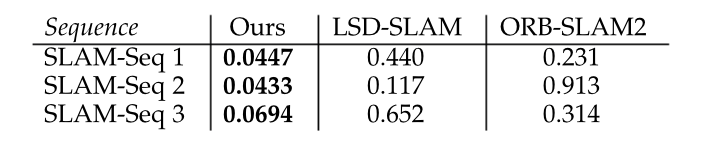
\includegraphics[width=0.5\linewidth]{./images/mm_errors.png}
    \caption{Marker Mapper absolute trajectory error (meters)}
    \label{fig:mmResults}
  \end{figure}

  The algorithm must first construct a map using off-line data. Once the transforms between tags are known, the map is used to report position from a known tag. The transforms between tags are corrected using redundant information in frames. The error along each basis cycle is computed, then an optimization algorithm is used to compute the corrected pose estimation. The mapping phase is an order of magnitude faster than Structure from Motion (SFM) and Multiple View Geometry (MVG) localization techniques. Although the paper mentions no on-line tests, is it reasonable to believe that pose estimation can be accomplished at minimally a 1Hz rate.

  Optical flow offers accurate angle measurements and fast updates that are relative to our current position. Like all camera based solutions, the vibration of the robot will likely makes this technique difficult. However, cameras are the most widely used sensor according to our survey of FRC students and alumni, which is another benefit of optical flow and tag based solutions. Optical flow can be applied either to cameras facing the environment or pointed down at the floor.

  The latter is the method used by computer mice, which have optical flow chips designed for high speed motion. Optical flow chips are made for optical flow detection with a specific lenses and microprocessor to get position \cite{font_characterization_2011}. These types of chips are built into computer mice with lenses that work only when the mouse is against a flat surface at a specific height from the table. This would be a problem in FRC since the field is not perfectly flat and there are sometimes obstacles that the robots need to drive over. There are also different drive trains which can shift center of balance between sets of wheels which would also cause the mouse to be off the ground. One of the benefits of using a mouse would the fast update rate. Optical flow mice update at 2,000 to 6,469 frames per second according to the ADNS-3080 optical flow sensors specifications \cite{sun_optical_2008}. They process frames quickly and most teams have mice of some sort they could use. However, a drawback of optical flow mice is their inability to detect rotation. Any rotational component in the optical flow is explicitly removed since computer users want only the translation of the mouse in order to navigate a computer screen. Lighting is also important to for the camera to be able to clearly pick up images so having a source of light illuminating around the optical flow mouse would also be necessary for teams in order to get the best results \cite{font_characterization_2011}.

  The other option for optical flow is to use a camera which faces the environment. This method is also sometimes called visual odometry. OpenCV provides libraries and sample programs for running dense optical flow and sparse optical flow in these configurations. Dense optical flow takes longer since it is using all of the points on a frame but can be more accurate \cite{itseez_opencv_2017}. In general, optical flow is not sufficient for localization on its own because it does not provide position in any global frame. However, environment-facing optical flow nicely complements our other systems because it uses a sensor we already plan to use (a simple webcam), and provides a source of local position updates not based on any assumptions about wheels or robot dynamics.

  \subsection{Proposed Localization Techniques} \label{section:proposed_techniques}

    Ultimately, we have identified IMUs, encoders, cameras with tags, beacons, and optical flow as promising techniques for localization in FRC. These techniques together provide redundant sources of both local and global pose estimates, and account for many of the challenges associated with localization for FRC. We believe that implementing each of these techniques and combining their results will produce a more robust localization than exploring any one of them in depth.




\section{Defining Successful Localization in FRC} \label{section:defining_success}

  Here we present the criteria a system must meet in order to be successful. Broadly, we consider the following factors to be those which are important, since they immediately effect the ability of an FRC team to use localization for interesting tasks.

  \begin{enumerate}
    \item \textbf{Accuracy}\\ How close our position estimates are to ground truth.
    \item \textbf{Precision}\\ How close repeated position estimates are to each other given the same ground truth.
    \item \textbf{Update Rate}\\ How quickly does our system provide position estimates.
    \item \textbf{Accessibility}\\ How affordable is our system, how difficult is it to make, and how easy is it for teams to use.
  \end{enumerate}

  A successful localization system for FRC should meet the following criteria:

  \begin{enumerate}
    \item \textbf{Accuracy} of $\pm$\SI{10}{\centi\meter} and $\pm$\ang{5}
    \item \textbf{Precision} of $\pm$\SI{5}{\centi\meter} and $\pm$\ang{2}
    \item \textbf{Update Rate} at \SI{20}{\milli\second}/50FPS, with global updates at \SI{100}{\milli\second}/10FPS
    \item \textbf{Accessibility} with cost under \$200 for teams.
  \end{enumerate}

  To come up with hard numbers for these criteria, we first performed a few simple calculations based on our knowledge of FRC and a survey we conducted. First, we consider what teams would want to use position information for, and decided that the applications requiring the most accuracy are shooting and autonomous pick of game pieces at known locations. Both of these require the position estimates to be close to the true position of the robot. From there, we estimate that most FRC shooting and pickup mechanisms will work within $\pm$\SI{10}{\centi\meter}. Next, we decided the application requiring the most precision would be path following. If position estimates are imprecise and jump around rapidly, smooth path following will be difficult. From our experience with path following, we estimated that $\pm$\SI{5}{\centi\meter} and  $\pm$\ang{2} would be sufficient. For update rate, we considered what the maximum distance a robot could move within a period and used that to decide what our update rate should be. The very fastest FRC robots move \SI{6}{\meter\per\second}, which at an update rate of every \SI{20}{\milli\second} is a distance of $0.02*6 =$ \SI{0.12}{\meter}. The rate of \SI{20}{\milli\second} is a realistic cycle time in FRC, and we feel \SI{12}{\centi\meter} is sufficient given the speed. For accessibility, we acknowledged that teams cannot spend more than \$400 on any part, and that they usually source parts from websites AndyMark, Cross-the-road Electronics, and National Instruments among other suppliers. We are also conscious that many FRC teams have limited or cluttered spaces for testing their robots, and may be working in a shared space that must be clean and usable after their work sessions.

  Using all of these informal estimates as a starting point, we conducted a survey of FRC students, alumni, and mentors. We received 65 responses in total, and used the results of this survey to solidify these design criteria. The full response of this survey are presented in \Newnameref{appendix:survey}. In summary, the median for accuracy was 4 inches in x,y and \ang{5} in yaw. Our survey did not include questions about precision and update rate, because they depend on what position is used for. Instead, we asked if students would try path planning if they had a localization system, which would back up our estimate of precision. Our survey indicated that 90\% of students would try to make the robot autonomously follow paths. Therefore, our precision estimated based on path planning as an application is supported by our survey. Update rate was not addressed in the survey because we didn't think FRC students would have informed opinions on this metric. Finally, we asked several questions about the accessibility requirements. A cost of under \$200 was deemed acceptable by 84.6\% of responses, and so we have made \$200 the goal for cost. Furthermore, we learned that the amount of space in teams shops varies from a 5 by 5 foot space up to several thousand square feet, but the median shop size is 775 $\text{ft}^2$, which one can imagine as a 25 by 30 ft space. In terms of access, about 76.5\% of teams could leave up tags or beacons, with the others stating that they must clean up everything because they work in a shared space such as a classroom. Lastly, we asked students what sensors they were familiar with. The most familiar sensors were cameras (90\%), followed by encoders (84.6\%), then IMUs (60\%). Therefore, it would be beneficial to incorporate cameras, encoders, and IMUs because teams are already familiar with them. However, in order to not place extra constraints on sourcing parts, we choose to ignore the constraint that the parts we test with meet the FRC-Legal or Off-The-Shelf requirements of FRC.

  Ultimately, we formulated design criteria based on our own experience with FRC and with localization, as well as by conducting a survey of the needs, experience, and opinions of FRC participants. These design criteria will help us pick which localization techniques to pursue as well as define a successful localization system for FRC.




\section{Experimental Results} \label{section:experiments}

  One of the key contributions of this MQP is an extensive set of empirical and theoretical results spanning the 5 different sensing technologies we outlined as promising (section \ref{section:proposed_techniques}). This section describes each of these experiments and explains how each test impacts the practical implementation of a complete localization system. Future projects working to implement an actual localization system for FRC can use these results to jump-start their development and inform design decisions.

  \subsection{Double Integration of Accelerometer is Inaccurate} \label{section:double_integration_is_inaccurate}

    We first demonstrate that double integration of raw accelerometer data is inaccurate. This is unsurprising, but for completeness we demonstrate specifically that double integration is inaccurate for the NavX IMU under FRC-like driving conditions. This inaccuracy comes from manufacturing errors, and electrical noise and imperfections in the IMU circuitry. Noise is also introduced from the vibrations of the robot chassis as it drives. Figure \ref{fig:double_integration} shows a typical example of naive trapezoidal rule to numerically double integrate the raw X and Y, with the rotation component coming from the yaw of the NavX which is very accurate (see \ref{section:yaw_accuracy}).

    \begin{figure}[H]
      \centering
      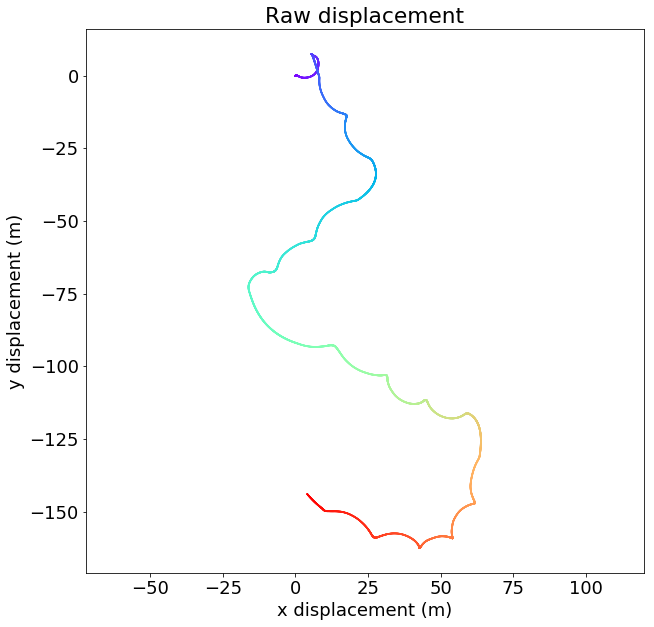
\includegraphics[width=0.8\linewidth]{./images/raw-displacement.png}
      \caption{The plot shows position by double integrating raw accerelometer readings. Time proceeds from purple to red. The truth path was a set of 7 mostly concentric 4m diameter circles. After the first ~1 seconds the data is inaccurate.}
      \label{fig:double_integration}
    \end{figure}

  \subsection{IMU Calibration} \label{section:imu_calibration}

    From an early experiment collecting data on a Turtlebot (section \ref{section:double_integration_is_inaccurate}), we saw that double integrating the accelerometer readings was not accurate enough. This was expected, because it is well known that double integration will amplify any bias. Therefore, we replicated the IMU calibration procedure described in \cite{tedaldi_robust_2014}, which accounts for many sources of error without requiring expensive external equipment. This calibration method was straightforward to perform, and could be replicated by FRC students. This calibration method corrects the misalignment, scaling, and biases in both accelerometer and gyroscope. This is done by optimizing for accelerometer calibration values that make the magnitude of acceleration during static intervals closest to 1, and then by optimizing for gyroscope calibration values that make the integral of gyroscope measurements between static intervals match the change in orientation between static positions. First, the IMU needed to be placed statically for a period of $T_{\text{init}}\approx50$ seconds. Next, by calculating the variance of the accelerometer data collected during that initialization period, a threshold for a static interval detector could be determined by applying a constant multiplier. After the initial waiting period, the IMU needs to be rotated an arbitrary amount and left in that orientation for 1 to 4 seconds. Each IMU position during the ``flip and wait'' period should be distinct for calibration to be accurate. The entire ``flip and wait'' process has to be repeated 36 to 50 times. After all data was collected, an optimization procedure was ran first on the accelerometer data to solve for the calibration parameters for misalignment, scaling, and bias that make the norm of the acceleration closest to 1. Then, a similar method was used for gyroscope calibration based on the success of accelerometer calibration. The quality of calibration of gyroscope was entirely based on the quality of the accelerometer calibration.

    In our experiments, we used $T_{\text{init}}=50$, as was reported by the authors for a different IMU. The authors arrived at this number from a plot of Allen Variance--we did not reproduce this plot with our IMU. We waited \SI{4}{\second} during our static intervals, but found that using $T_{\text{wait}}=3$ was better in practice for detecting wide, clean, static intervals. This is possibly because a sometimes the IMU was not truly at rest for a full four seconds. In our early experiments, we found that failing to record enough \textit{distinct} static intervals would cause the optimization procedure to fail to converge. So, in order to get as many distinct positions as possible, a Helping-Hands was used to hold the IMU. We rotated the IMU 36 times in total, which was the minimum suggested number of static intervals in the original paper. The accelerometer data and gyroscope data in $x$, $y$, and $z$ axis were recording for the entire period. Using the threshold from initialization data and the full accelerometer data, the static detector successfully distinguished between static intervals and dynamic intervals. A demonstration of our static detector is shown in Figure \ref{fig:static_detector}.

    \begin{figure}[H]
      \centering
      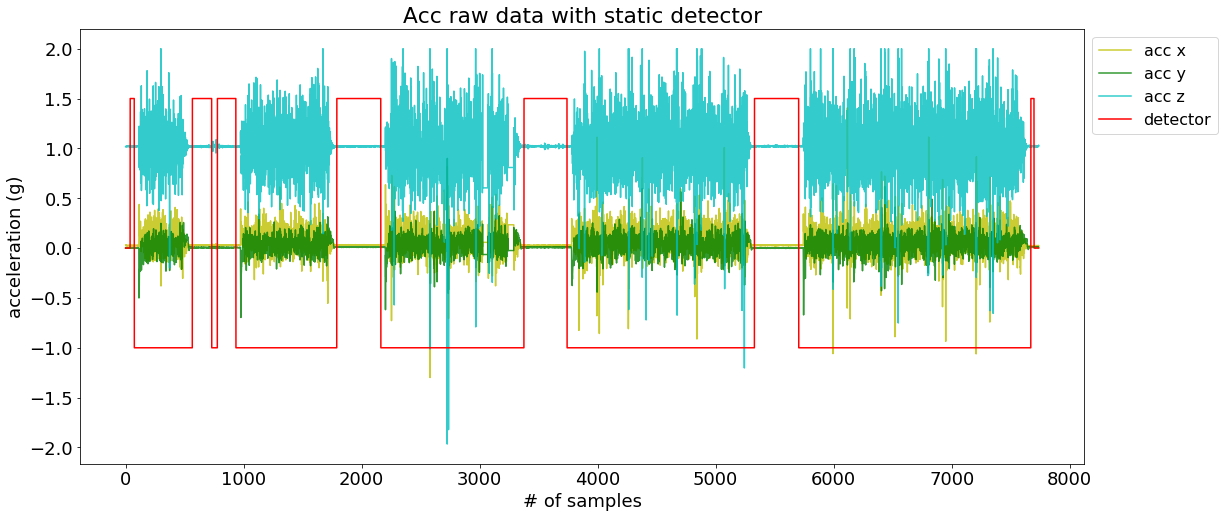
\includegraphics[width=1\linewidth]{./images/static_detector.png}
      \caption{The black line is 1 during intervals classified as static}
      \label{fig:static_detector}
    \end{figure}

    Using the identified static intervals, we optimize using the Levenburg-Marquedt procedure in python's NumPy package to solve for the accelerometer calibration values. The equation we are minimizing is shown below (Equation \ref{eq:accel_calibration_error}). These values can be found in Table \ref{table:imu_calibration_values}, and descriptions of each variable can be found in \cite{tedaldi_robust_2014}.

    \begin{equation} \label{eq:accel_calibration_error}
      \rVert g\lVert^2 - \rVert T^aK^a(a^s+b^a)\lVert^2
    \end{equation}

    \begin{table}[H]
      \centering
      \resizebox{\textwidth}{!}{
      \begin{tabular}{|c|c|c|c|c|c|c|c|c|}
        \hline
        $\alpha_{yz}$ & $\alpha_{zy}$ & $\alpha_{zx}$ & $s^a_x$ & $s^a_x$  & $s^a_z$ & $b^a_x$ & $b^a_y$ & $b^a_z$ \\
        \hline
        -0.002710 & 0.004559 & -0.000738 & 0.997279 & 0.996661 & 0.989960 & -0.006376 & -0.008999 & -0.019918 \\
        \hline
      \end{tabular}}
      \caption{IMU Calibration Values}
      \label{table:imu_calibration_values}
    \end{table}

    Note the values shown above are close to the values that represent no transformation, $[0, 0, 0, 1, 1, 1, 0, 0, 0]$. This indicates that our accelerometer is already quite well calibrated but not quite perfect, which is expected.

    The next step is to calibrate the gyroscope. We integrate the angular rates measured by the gyro between every sequential pair of static intervals and compare this to the angle between the two static intervals. We have a good estimate of the true orientation of each static interval from the previous accelerometer calibration step, and so the goal is to solve for gyroscope calibration parameters that make the integral of the transformed gyroscope data over the dynamic interval match the next orientation of the static interval as measured from the calibrated accelerometer readings. This is expressed in the error function we are minimizing, shown in Equation \ref{eq:gyro_calibration_error}.

    \begin{equation} \label{eq:gyro_calibration_error}
      \begin{split}
        % FIXME: this equation looks wrong
        \bigg\lVert u_{a,k} - \bigg(\int_{k-1}^{k} \Omega(\omega^S_i)di + u_{a,k-1}\bigg) \bigg\lVert \\
      \Omega(\omega^S_i) = T^gK^g(\omega^S_i+b^g)
      \end{split}
    \end{equation}

    The function $\Omega(\omega^S_i)$ takes the raw angular velocity readings $w^S_i$, transforms them with the calibration constants, and produces a rotation matrix. This rotation matrix is the euler rotation matrix (Roll-Pitch-Yaw ordering) which can then be multiplied by $u_a$. Towards this process, we investigated numerical methods for computing the above integral. This integral cannot be computed analytically because we only have samples of the integrad, rather than a analytic closed-form. Therefore, numerical integration methods like Euler's Forwardmethod or Runga-Kutta methods can be used. While \cite{tedaldi_robust_2014} uses Runga-Kutta 4th Order (RK4), we used the 1-step Euler's Forward method. Over the whole integral, this rotates the average acceleration values from the $k-1$th static interval, $u_{a,k-1}$, to the average acceleration values from the $k$th static interval. One could compute the same thing in a different order, by integrating the angular velocity values to get angles, constructing one rotation matrix, then rotating the acceleration values. However, because of gimble lock and dependence on ordering of the axis of rotation, this is much less accurate in practice. By rotating within the ingrand, we are only rotating by very small angles at a time, which mitagates the issues of using euler-angle rotation matrices. This theoretical result was tested experimentally, and the results are shown in Figure \ref{fig:gyro_integration}. Note that the bars representing the incremental rotation are more accurate than the one-shot rotation, where more-accurate is defined as closer to the true average acceleration readings at the next frame.

    \begin{figure}[H]
      \centering
      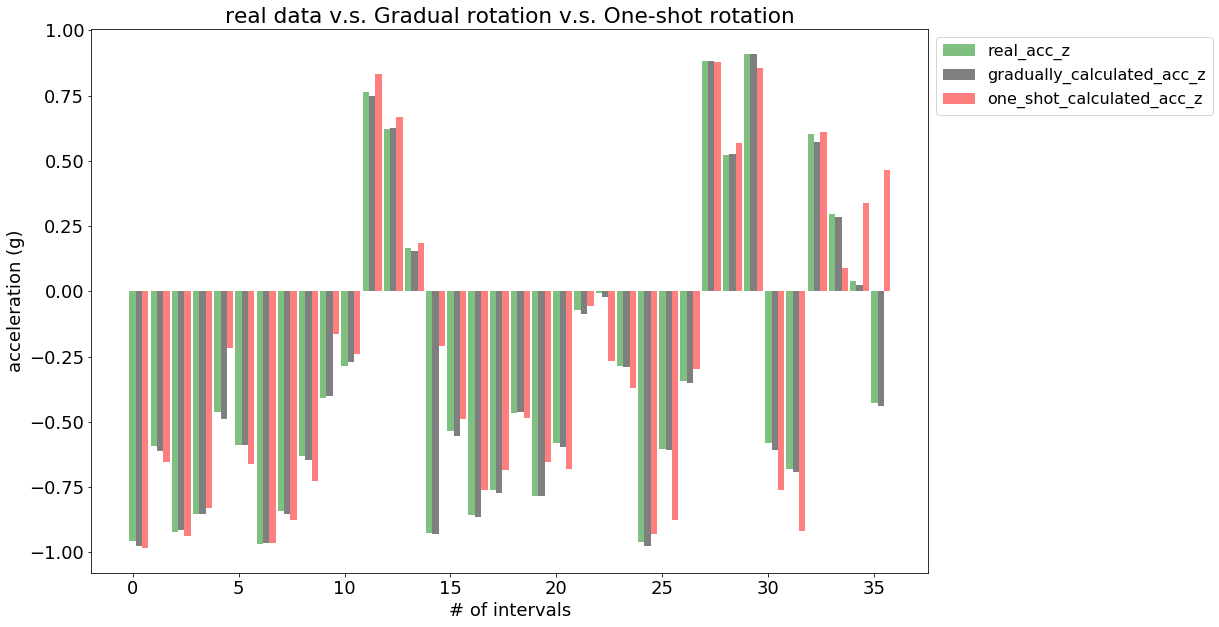
\includegraphics[width=1\linewidth]{./images/gyro_integration_y.png}
      \caption{Integration of the gyroscope readings in the Y Axis. Method 1 is one-shot rotation, Method 2 is incremental rotation. Incremental rotation is clearly more accurate.}
      \label{fig:gyro_integration}
    \end{figure}

  \subsection{Accuracy of Gyro Integration versus On-Chip Yaw Calculation} \label{section:yaw_accuracy}

    We asked the question of whether the provided on-chip \texttt{GetYaw()} method is more or less accurate than what can be computed from the raw gyroscope readings. To answer this question, we first used implemented a simple procedure for computing yaw from the gyroscope readings. First, we apply the calibration parameters (see section \ref{section:imu_calibration}), then a base-frame rotation. This base frame rotation accounts for the angle of mounting of the NavX on our robot, which may not be perfectly flat. To do this, we let the robot sit still for a second or two and compute the rotation matrix that rotates the accelerometers readings to be $[0,0,1]$, which is the value you'd expect if the NavX were flat. Having calibrated and rotated the raw gyroscope readings in all axis, we can consider only the yaw, or $z$ axis, of the rotated data. We use a 1-step forward Euler's method to integrate these readings, which are in degrees/second. This gives us our yaw angle over time.

    To compare this procedure with ground truth, we log the raw gyro values values while driving in the motion capture studio, then perform the calculations described above to get yaw. Figure \ref{fig:yaw_comparison} shows our computed yaw, compared with the on-chip \texttt{GetYaw()} and the yaw reported by motion capture. Due to the wrap-around behavior, the mocap yaw has a small blip in value that can be ignored. Overall, both our yaw value and \texttt{GetYaw()} match the ground truth very closely. The maximum error of \ang{2.497} in the first 1000 samples (20 seconds).

    \begin{figure}[H]
      \centering
      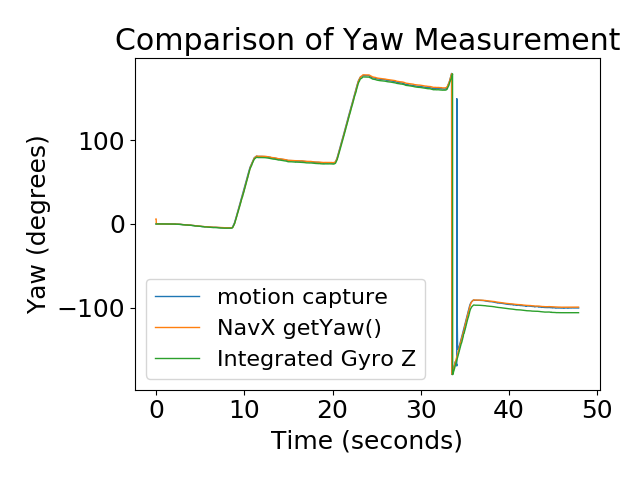
\includegraphics[width=0.49\linewidth]{./images/yaw_comparison_2.png}
      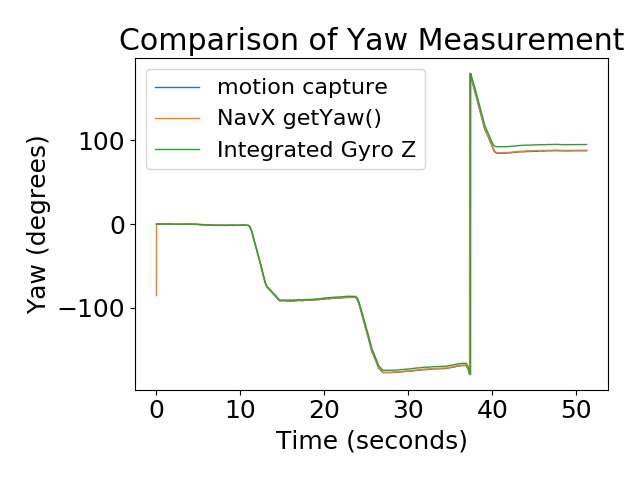
\includegraphics[width=0.49\linewidth]{./images/yaw_comparison_3.png}
      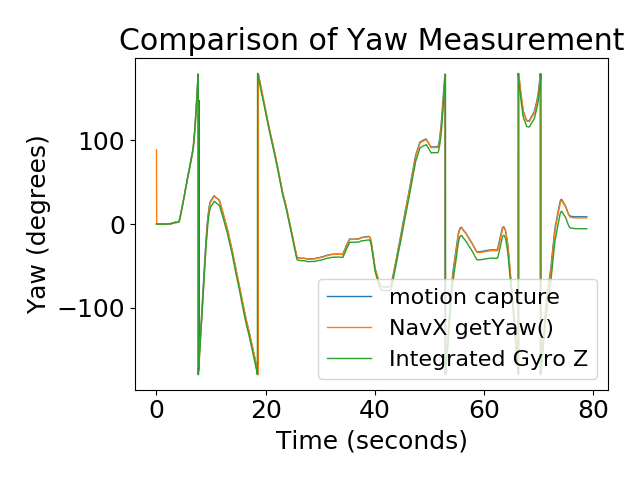
\includegraphics[width=0.49\linewidth]{./images/yaw_comparison_4.png}
      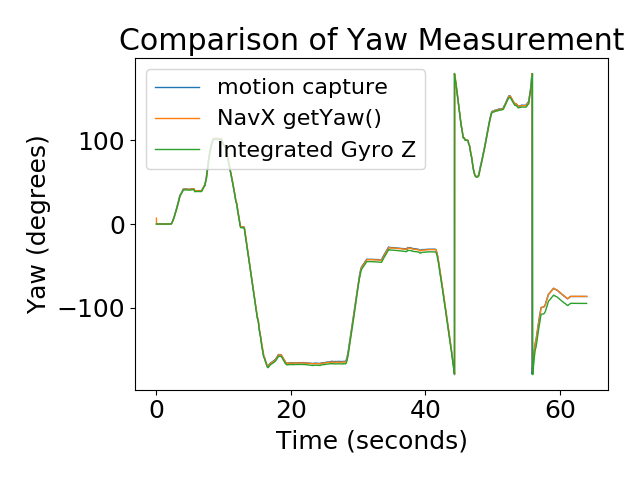
\includegraphics[width=0.49\linewidth]{./images/yaw_comparison_5.png}
      \caption{Comparison of yaw values between our algorithm and motion capture. The \texttt{GetYaw()} and Motion Capture lines are nearly indistinguishable.}
      \label{fig:yaw_comparison}
    \end{figure}

    \begin{table}[H]
      \centering
      \begin{tabular}{|c|c|c|c|} \hline
        Trial & Data Source & Average Error (deg) & 90th Percentile Error (deg) \\ \hline
        1 & Navx \texttt{GetYaw()} & 1.275 & \textbf{4.606} \\ \hline
        2 & Navx \texttt{GetYaw()} & 1.027 & \textbf{2.298} \\ \hline
        3 & Navx \texttt{GetYaw()} & 1.402 & \textbf{3.591} \\ \hline
        4 & Navx \texttt{GetYaw()} & 1.458 & \textbf{4.032} \\ \hline
        1 & Integrated & 3.619 & 7.710 \\ \hline
        2 & Integrated & 2.670 & 5.589 \\ \hline
        3 & ntegrated & 6.315 & 13.659 \\ \hline
        4 & Integrated & 3.182 & 8.206 \\ \hline
      \end{tabular}
      \caption{Table of errors during 4 trials of the NavX on a Turtlebot under motion capture. The NavX is more accurate than integration and meets our criteria of accurate angle measurement (see section \ref{section:defining_success}).}
      \label{}
    \end{table}

  \subsection{Characterising Drift and Bias in the Accelerometer}

    After confirming experimentally that integrating accelerometer readings would be innacurate, we explore the well known techniques of drift compensation and zero velocity updates. Before testing these directly, we first categorize just how much bias there is in our accelerometer, and how that bias changes over time.

    \subsubsection{Measuring the drift and bias in the accelerometer} \label{section:drift_bias}

      Compensating for the accelerometer drift is important in IMU localization since double integration of accelerometer data amplifies any inaccuracies. We first performed an experiment to study the drift of accelerometer when it is stationary. We put the accelerometer on a flat surface for 6 minutes and collected the data at \SI{100}{\hertz} (see Figure \ref{fig:static_test}). Then, we calculated the average accelerometer value of the first 500 samples and the last 500 samples in the x and y axes. The difference of mean values of first 500 samples and last 500 sample in x, y, z axes are -0.000475g, 0.000158g, 0.000323g respectively. For reference, we note that the maximum drift of -0.00475g, or \SI{-0.00465}{\meter\per\second\squared} would cause a position error of $0.5*-0.00465*3^2=$\SI{-0.020948}{\meter} over a 3 second period. In other words, if the NavX is stationary, even if the initial bias of the accelerometer is zero, the position could drift up to \SI{2}{\centi\meter} over 3 seconds.

      \begin{figure}[H]
        \centering
        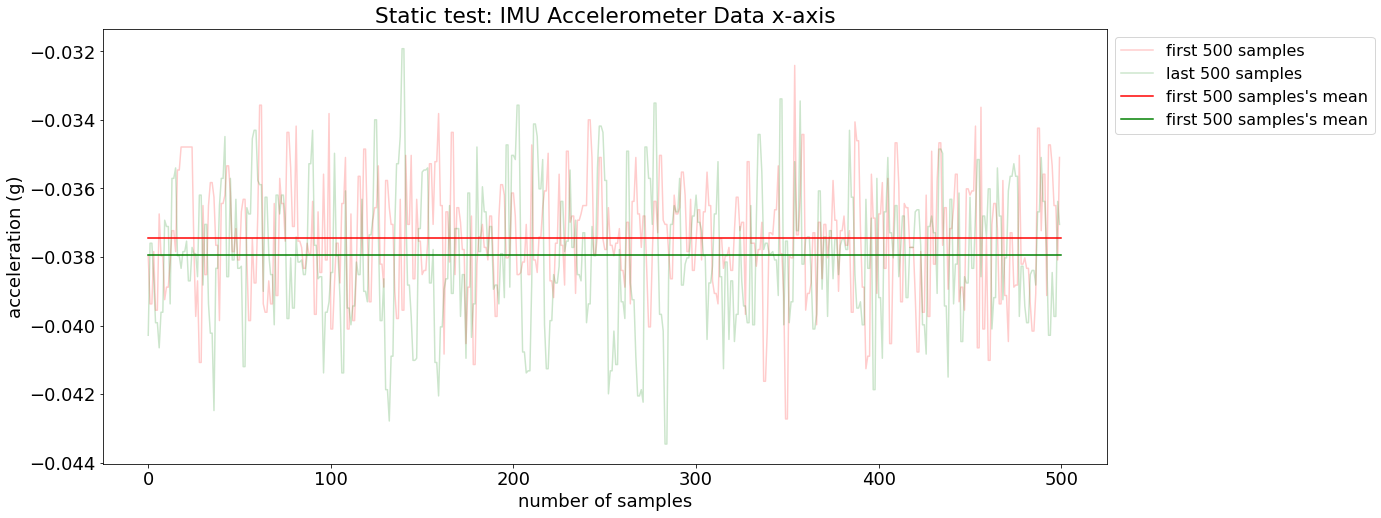
\includegraphics[width=1\linewidth]{./images/static_test.png}
        \caption{The raw measured X acceleration (Gs) and its mean over first and last 500 sample periods while stationary.}
        \label{fig:static_test}
      \end{figure}

      We then wondered that whether the duration of motion influences the amount of drift, so we performed another experiment. We drove the robot in a circle, stopped for 9 seconds, drove the robot in 2 circles, stopped for 9 second, so on until the robot drove for 5 circles in a row. We will refer to this test as the ``Nypro Circles'' test. This allows us to see whether moving for longer periods of times will cause more drift. We collected the accelerometer data, fused yaw measurement, and temperature. Using this data, we plot the mean accelerometer value in each of the static intervals to see if there is a clear trend (see Figure \ref{fig:static_means}). Based on these means, we can say that the NavX accelerometer drifted a lot between static intervals. However, there is no simple linear trend between the duration of motion.

      \begin{figure}[H]
        \centering
        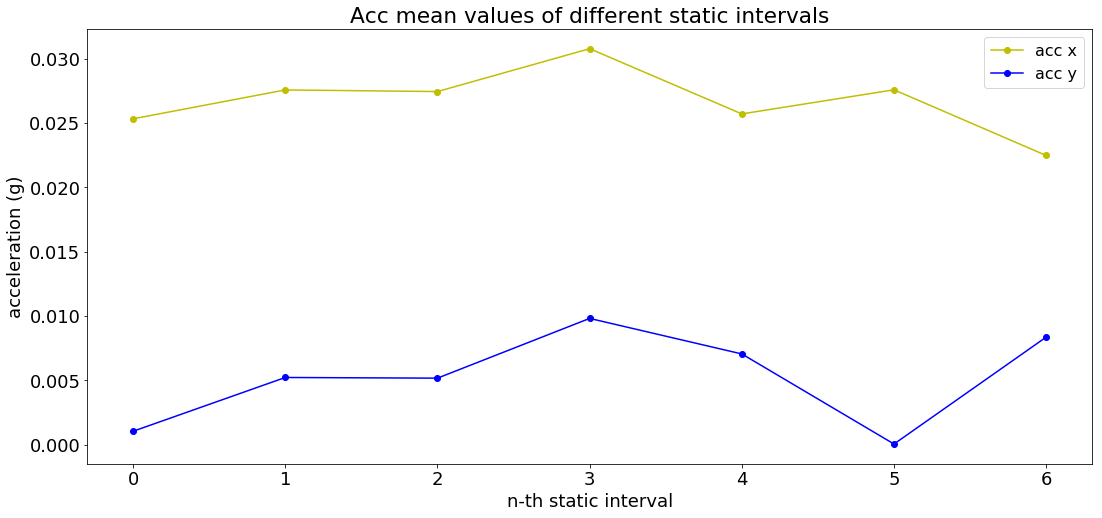
\includegraphics[width=1\linewidth]{./images/static_means.png}
        \caption{The means of the accelerometer data in world-frame X and Y in each static interval.}
        \label{fig:static_means}
      \end{figure}

      Having measured the accelerometer bias and studied its drift, we then integrated the accelerometer data with yaw angles of the ``Nypro Circles'' test to see how these effect the position. To get the best results possible, we also apply our calibration parameters (see \ref{section:imu_calibration}). When integrating to get position, we rotate the robot into the world frame using the yaw angles come from the \texttt{GetYaw()} function of the NavX API, which is very accurate (see \ref{section:yaw_accuracy}. Figure \ref{fig:calibrated_velocity} and \ref{fig:calibrated_displacement} show that bias and drift make velocity and displacement inaccurate after only a short period of motion.

      \begin{figure}[H]
        \centering
        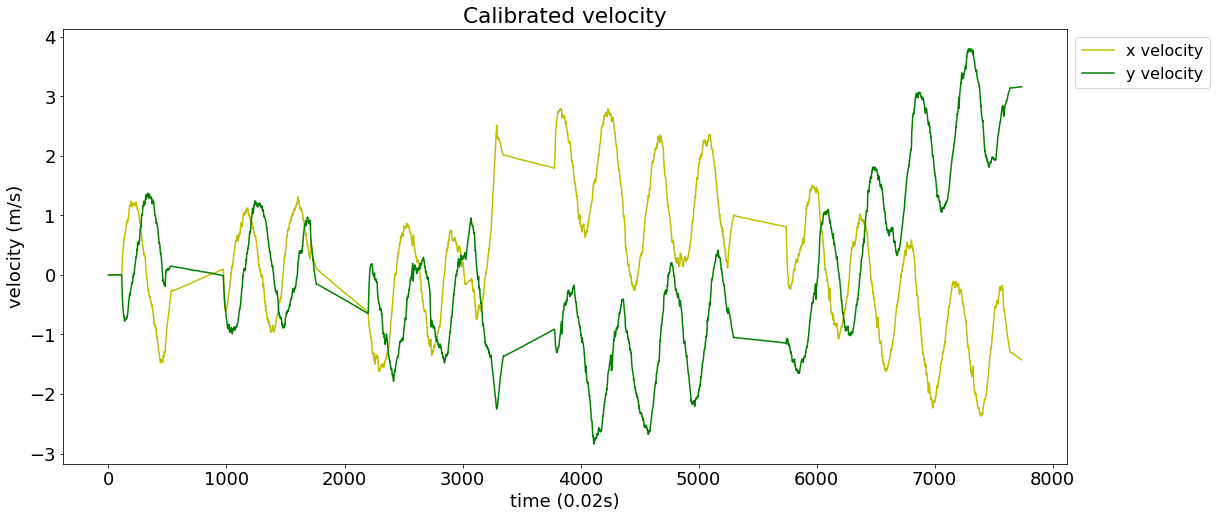
\includegraphics[width=1\linewidth]{./images/calibrated_velocity.png}
        \caption{Velocity as derived by integrating the calibrated accelerometer measurements.}
        \label{fig:calibrated_velocity}
      \end{figure}

      \begin{figure}[H]
        \centering
        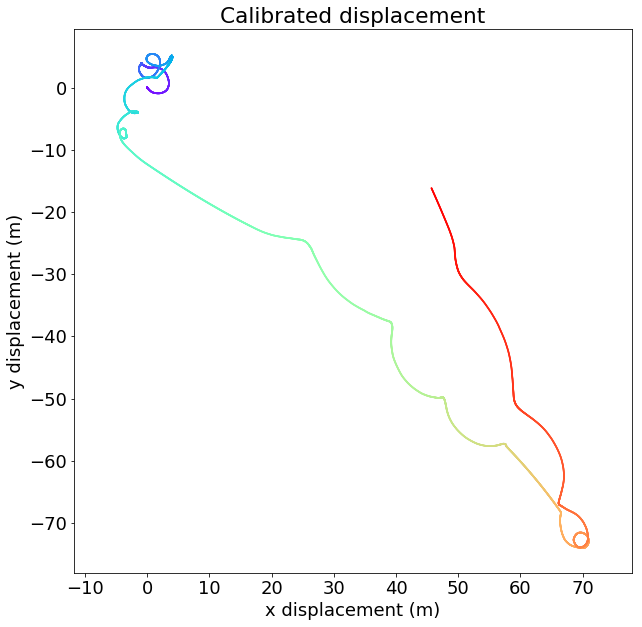
\includegraphics[width=0.6\linewidth]{./images/calibrated_displacement.png}
        \caption{Displacement as derived by twice-integrating the calibrated accelerometer measurements.}
        \label{fig:calibrated_displacement}
      \end{figure}

      Since temperature could also be a factor that affects accelerometer values, we compared the temperature with accelerometer values in static intervals over time. Shown in Figure \ref{fig:temperature}, the temperature increased when the robot was static and decreased when the robot was in motion. However, temperature does not have a straightforward relationship with accelerometer bias or drift in bias.

      \begin{figure}[H]
        \centering
        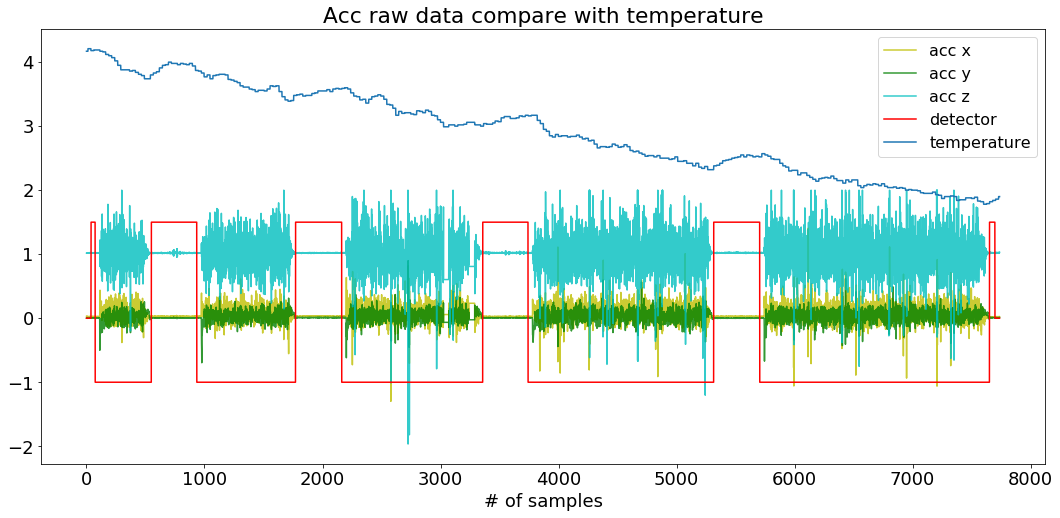
\includegraphics[width=1\linewidth]{./images/temperature.png}
        \caption{A Plot of temperature recorded by the NavX over the duration of our test.}
        \label{fig:temperature}
      \end{figure}

      Overall, our experiments showed that the accelerometer is subject to bias, and that these biases drift over periods of motion. Because of these errors, the double integration becomes inaccurate after a very short duration of motion. Furthermore, we show that the magnitude and direction of this drift has no straightforward relationship with the duration of motion or temperature. We now present several approaches for handling these sources of error and describe our results applying them to this data.

    \subsubsection{Zero Velocity Updates} \label{section:zero_velocity_updates}

      Looking at the calibrated velocity plots (Figure \ref{fig:calibrated_velocity}), clearly there is still bias in the accelerometer readings which are causing the velocity to drift up and down during intervals of motion. We now apply zero velocity updates to the data to mitigate this. Our zero velocity updates work as such: when the static detector indicates the robot is stationary, calculate the bias in that static interval, remove that bias from the static interval and the following dynamic interval, and finally set the current velocity estimate to be zero. %TODO: add more details or math on how precisely this is done

      \begin{figure}[H]
        \centering
        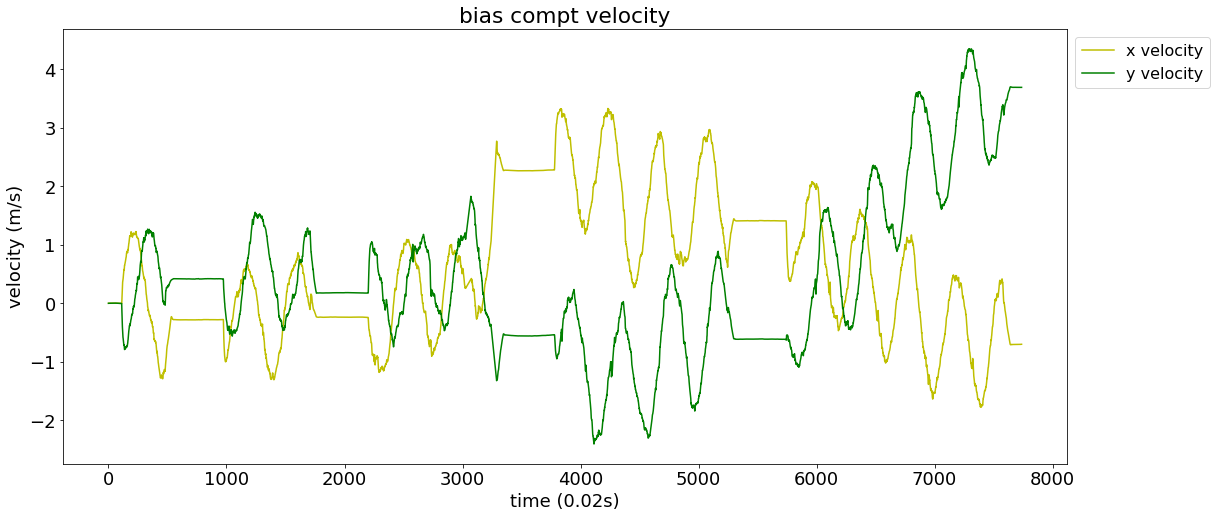
\includegraphics[width=1\linewidth]{./images/bias-compt-velocity.png}
        \caption{Velocity after bias during static intervals is removed.}
        \label{fig:bias-removed}
      \end{figure}

      \begin{figure}[H]
        \centering
        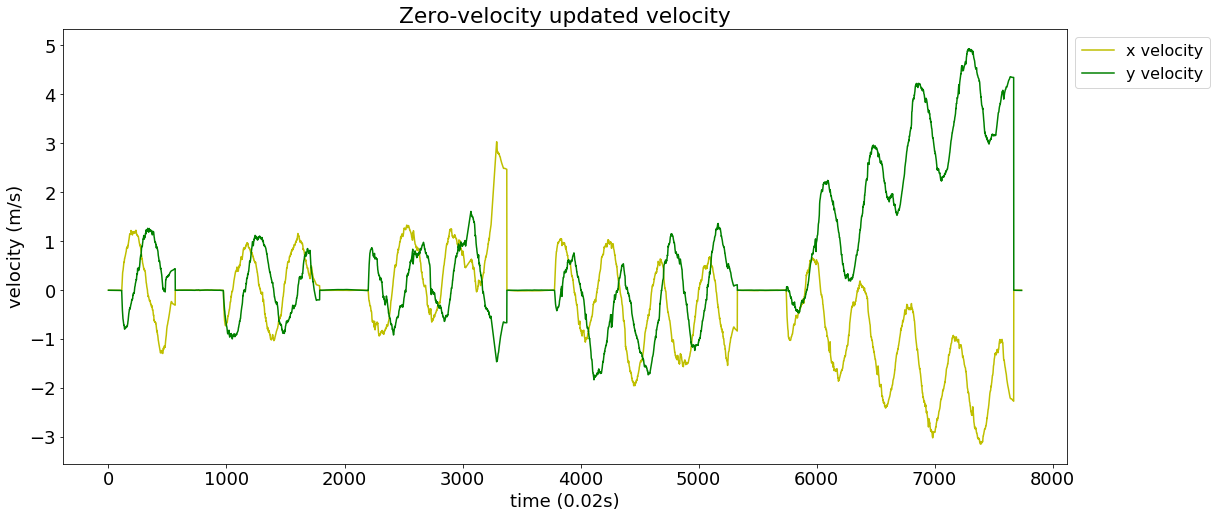
\includegraphics[width=1\linewidth]{./images/zeroed-velocity.png}
        \caption{Velocity after both applying bias and zeroing velocity estimates.}
        \label{fig:zeroed_velocity}
      \end{figure}

    \subsubsection{Drift Compensation}

      Having compensated for the biases found during static intervals, we now wonder whether we can account for the drift between these static interval biases. As was shown in Section \ref{section:drift_bias}, there is no clear trend in how the motions change between or within static intervals. This means we cannot hope to find any one drift rate and apply it to the entire stream of accelerometer data. However, there are two other possible ways to account for drift looking only at a single static interval or a single pair of static intervals. The first method is to calculate the drift rates \textit{between} two sequential static intervals, and apply drift compensation starting from the static interval and up until the next static interval. This method is an offline method since it requires knowing the future accelerometer data to account for the drift in the current data. Because this method requires future data, it is not possible to implement in our system in real time. The second method is to calculate the drift rate \textit{within} a static interval and project this drifting behavior on both the static interval and the following dynamic interval. This method is online because it only requires current and past accelerometer readings. Both of these methods offer no significant improvement, but we report them for completeness. These two methods are plotted below, with the original data (only calibration applied, no drift compensation) shown for comparison (Figures \ref{fig:calibrated_velocity_ref}, \ref{fig:offline_drift_compensation}, \ref{fig:online_drift_compensation}).

      \begin{figure}[H]
        \centering
        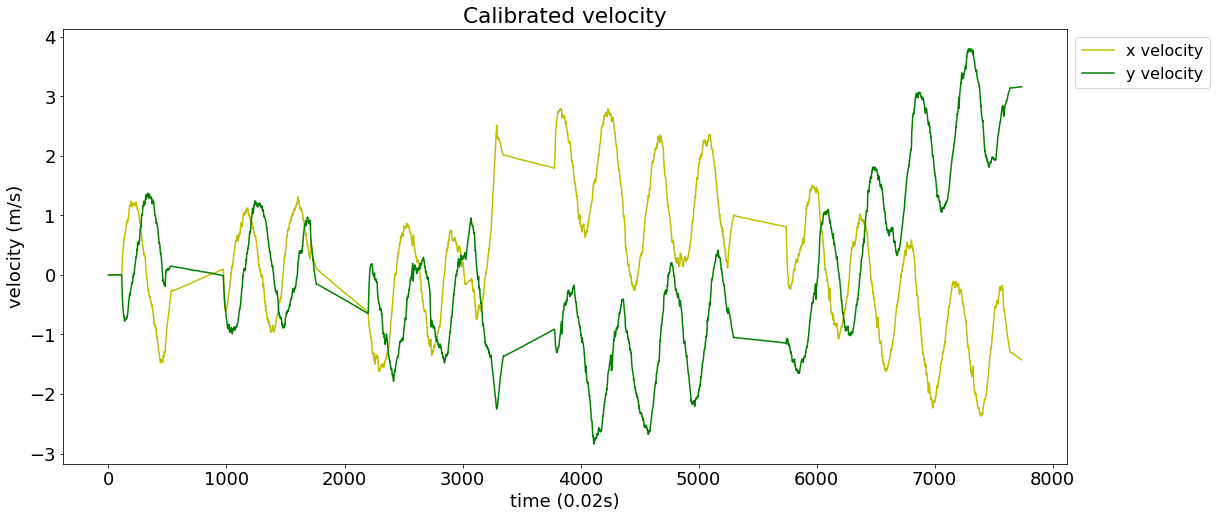
\includegraphics[width=0.85\linewidth]{./images/calibrated_velocity.png}
        \caption{Velocity as derived by integrating the calibrated accelerometer measurements.}
        \label{fig:calibrated_velocity_ref}
      \end{figure}

      \begin{figure}[H]
        \centering
        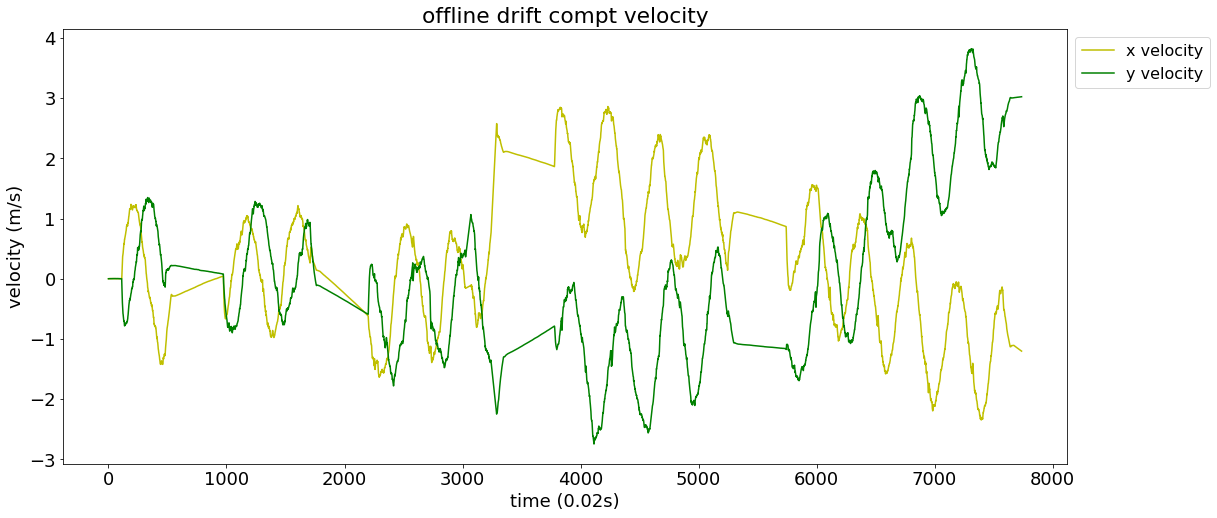
\includegraphics[width=0.85\linewidth]{./images/offline_drift_compensation.png}
        \caption{Velocity where drift is calculated between static intervals}
        \label{fig:offline_drift_compensation}
      \end{figure}

      \begin{figure}[H]
        \centering
        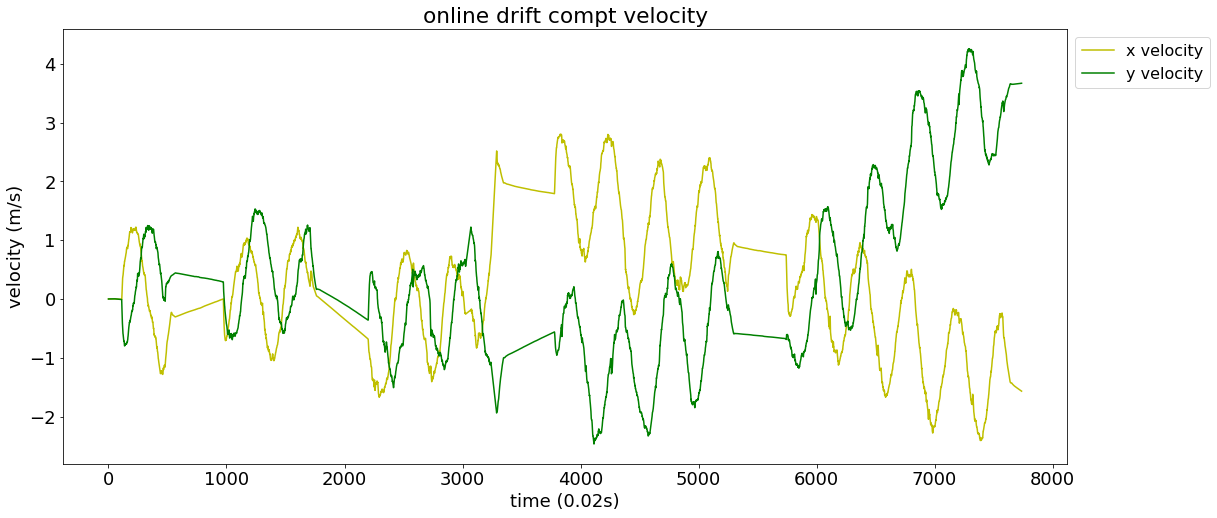
\includegraphics[width=0.85\linewidth]{./images/online_drift_compensation.png}
        \caption{Velocity where drift is calculated within static intervals}
        \label{fig:online_drift_compensation}
      \end{figure}

  \subsection{Comparing Our IMU Localization to the NavX API}

		% TODO: also compare using with new mocap data

		We compare our method for localization with only the IMU against the \texttt{GetWorldX()} and \texttt{GetWorldY()} functions provided by the NavX. These functions differ from our methods because they do not include zero velocity updates or drift compensation. We also apply our own calibration parameters to our data, which differs from the internal calibration done by the NavX. As is shown in the Figure \ref{fig:displacement_comparison}, both methods drift significantly over the course of our experiment (``Nypro Circles'', described in Section \ref{section:drift_bias}). For reference, in this test our robot was driven in circles with a constant left-right wheel speed difference. However, when we zoom in to the first thirty seconds of the data, we see our method better preserves the sinusoidal nature of the motion, whereas the NavX position constructs lots of straight edges. Furthermore, zooming in to the first three seconds highlights that our method is significantly more accurate.

		\begin{figure}[H]
			\centering
			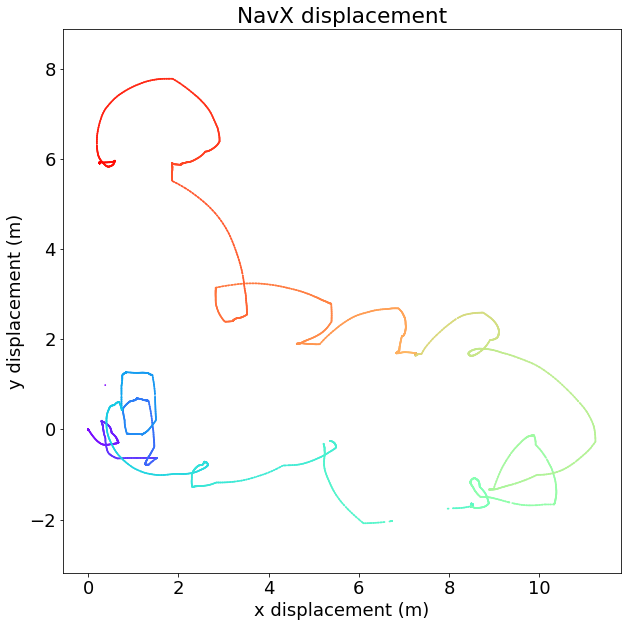
\includegraphics[width=0.49\linewidth]{./images/navx-displacement.png}
			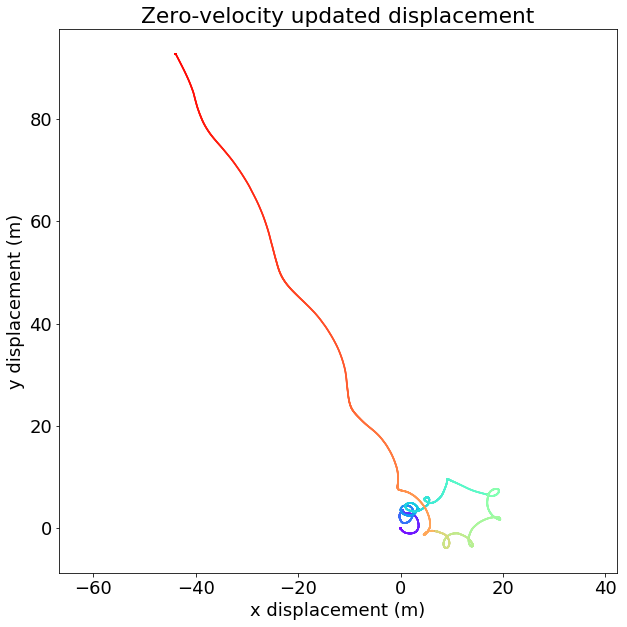
\includegraphics[width=0.49\linewidth]{./images/zeroed-displacement.png}
			\caption{Comparison between NavX (left) and our method (right) over the entire experiment.}
			\label{fig:displacement_comparison}
		\end{figure}

		\begin{figure}[H]
			\centering
			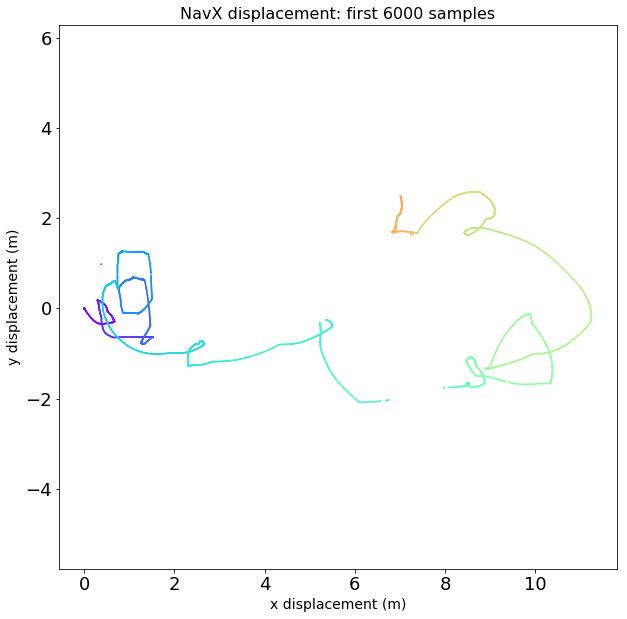
\includegraphics[width=0.49\linewidth]{./images/navx-displacement-30s.png}
			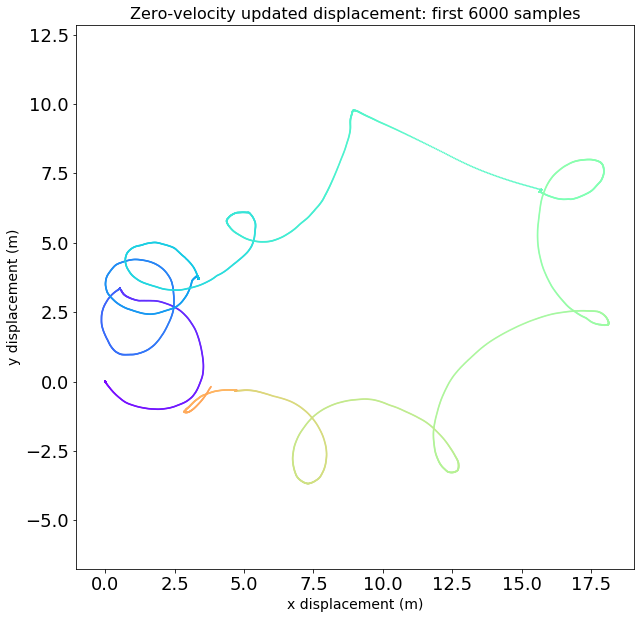
\includegraphics[width=0.49\linewidth]{./images/zero-displacement-30s.png}
			\caption{Comparison between NavX (left) and our method (right) over the first 30 seconds of the experiment.}
			\label{fig:displacement_comparison_30s}
		\end{figure}

		\begin{figure}[H]
			\centering
			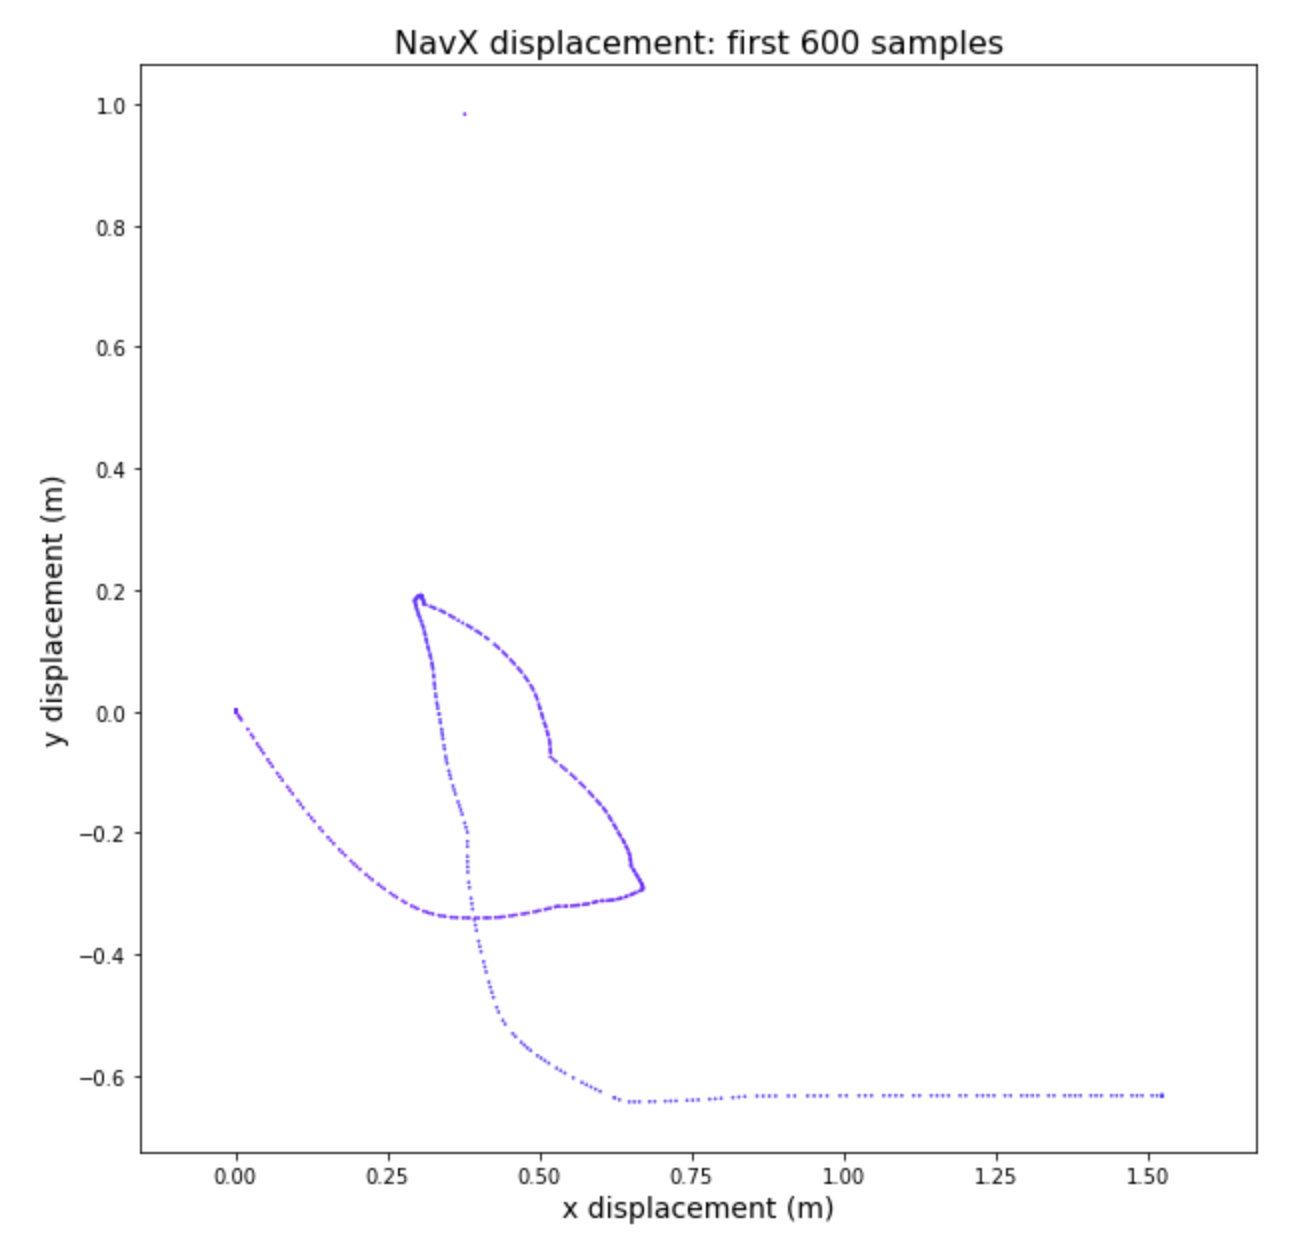
\includegraphics[width=0.49\linewidth]{./images/navx-displacement-3s.png}
			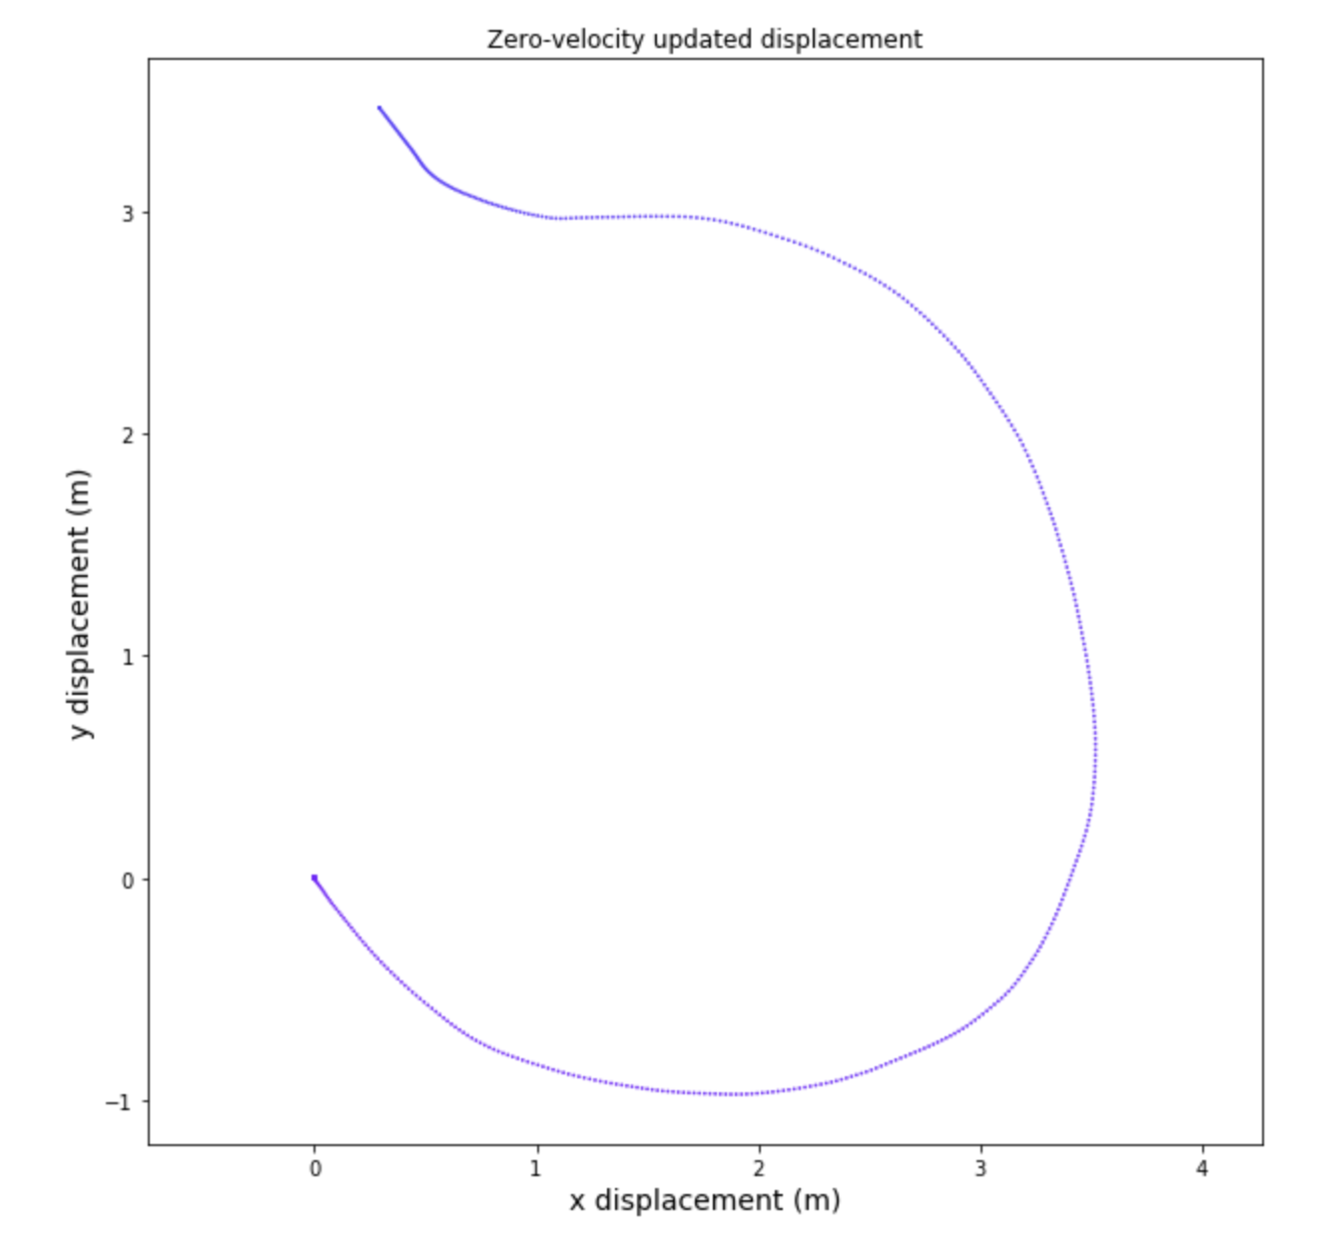
\includegraphics[width=0.49\linewidth]{./images/zero-displacement-3s.png}
			\caption{Comparison between NavX (left) and our method (right) over the first 3 seconds of the experiment.}
			\label{fig:displacement_comparison_3s}
		\end{figure}

  \subsection{Measuring Beacon Delays}

    The beacon system relies on measuring the time it takes for a sound signal to travel from the beacons to the robot. To do this accurately, one must account for transmit and receive delays in addition to the actual time of flight. Figure \ref{fig:rx_tx_timing} illustrates the various delays we need to account for. We conducted experiments to estimate these delays.

      \begin{figure}[H]
        \centering
        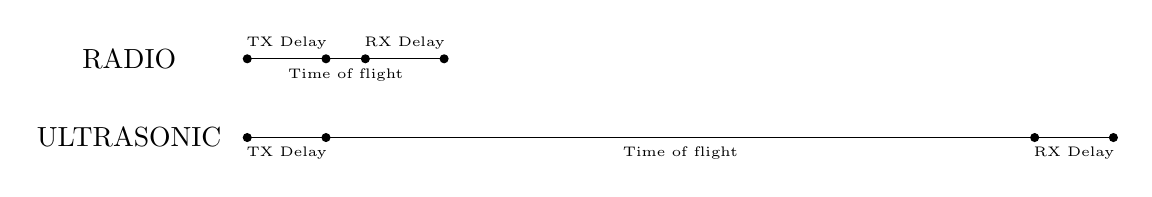
\begin{tikzpicture}
          % timeline for ultrasonic
          \draw (-1.5, 0) node {ULTRASONIC};
          \filldraw (0,0) circle (0.05);
          \draw (0.5, -0.2) node {\tiny TX Delay};
          \draw (0,0) -- (1,0);
          \filldraw (1,0) circle (0.05);
          \draw (5.5, -0.2) node {\tiny Time of flight};
          \draw (1,0) -- (10,0);
          \filldraw (10,0) circle (0.05);
          \draw (10.5, -0.2) node {\tiny RX Delay};
          \draw (10,0) -- (11,0);
          \filldraw (11,0) circle (0.05);

          % timeline for radio
          \draw (-1.5, 1) node {RADIO};
          \filldraw (0,1) circle (0.05);
          \draw (0.5, 1.2) node {\tiny TX Delay};
          \draw (0,1) -- (1,1);
          \filldraw (1,1) circle (0.05);
          \draw (1.25, 0.8) node {\tiny Time of flight};
          \draw (1,1) -- (1.5,1);
          \filldraw (1.5,1) circle (0.05);
          \draw (2.0, 1.2) node {\tiny RX Delay};
          \draw (1.5,1) -- (2.5,1);
          \filldraw (2.5,1) circle (0.05);
        \end{tikzpicture}
        \caption{Timing of radio and ultrasonic signals. Experiments indicate \SI{46.175}{\micro\second} total RF delay and \SI{1}{\milli\second} total ultrasonic delay.}
        \label{fig:rx_tx_timing}
      \end{figure}


    First, to get an estimate of the radio transmit and receive delay, a transmitter and receiver were set up on two microcontrollers. The transmitter sent \SI{5}{\milli\second} pulses at \SI{433}{\mega\hertz} (no encoded data) every \SI{55}{\milli\second}, and oscilloscope probes were attached to the input pin on the transmitter and the output pin on the receiver. By comparing the time difference between the input and output signals on the oscilloscope, we can determine the total time. Furthermore, we can measure the distance between the transmitter and receiver and subtract the theoretical time of flight from the total time. The full data for these measurements are available in \Newnameref{appendix:rf-rx-tx}, and an example measurement is shown in Figure \ref{fig:rf_delay_ex}. The time of flight of radio over distances of a new centimeters or meters is on the order of nanoseconds. We measured an average delay of \SI{45.175}{\micro\second}, which we attribute to the internal circuitry of the transmitter and receiver. The variance of this delay was \SI{16}{\micro\second}. However, we also measured delays as low as \SI{32}{\micro\second} and as high as \SI{79}{\micro\second}. Since the theoretical time of flight over the distances used in this experiment were at most \SI{1}{\nano\second}, we can conclude that there is both delay and significant variance in the delay of the transmitters and receivers. This is an important delay to consider when implementing the timing measurement of the beacon signals.

    \begin{figure}[H]
      \centering
      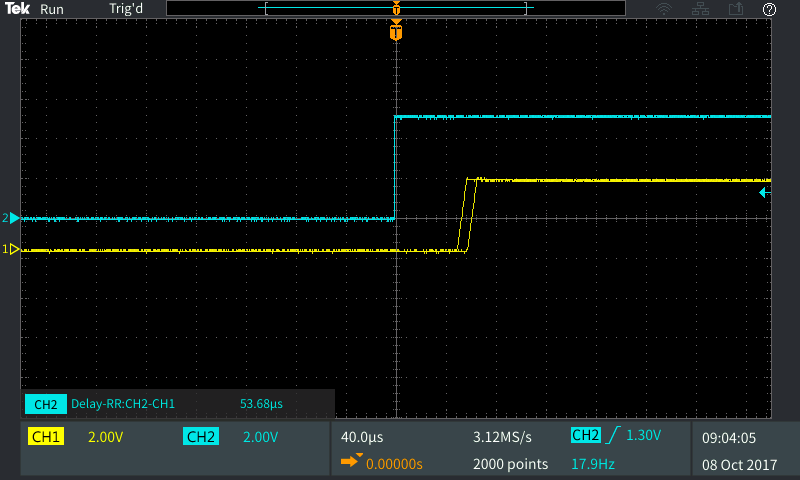
\includegraphics[scale=0.2]{./images/rf_delay_ex.PNG}
      \caption{Example measurement total trip time for radio signal. The blue line is the input to the transmitter, and the yellow are the output of the receiver}
      \label{fig:rf_delay_ex}
    \end{figure}

    Next we performed a similar experiment with the ultrasonic transducers. For this experiment, we used two NTX-1004PZ piezo speakers placed \SI{25}{\centi\meter} apart. The NTX-1004PZ is meant to be a high-frequency speaker for DJ equipment, and is designed to operate between \SI{4}{\kilo\hertz} and \SI{20}{\kilo\hertz}. However, because they are incredibly cheap we decided to evaluate them as ultrasonic speakers running just above that range. One was connected to a PSoC 5LP for transmitting, and the other was connected only to the oscilloscope. The other oscilloscope probe was connected to the transmitting piezo. The time difference between the transmitting signal and the receiving signal was measured. The signal applied to the transmitter was short bursts of a 24Hz square wave. Again, the distance was measured between the transmitted and received waveform, and the theoretical time of flight was subtracted. The full data for this experiment is shown in table \ref{table:us_delay}.

    \begin{table}[H]
      \centering
      \begin{tabular}{|c|c|c|c|}\hline
        Distance (m) & Expected Delay (us) & Measured Delay (us) & Error (Measured - Expected) \\ \hline
        0.10 & 294 &  390 &  96 \\ \hline
        0.15 & 441 &  556 & 115 \\ \hline
        0.20 & 588 &  698 & 110 \\ \hline
        0.25 & 735 &  872 & 137 \\ \hline
        0.30 & 882 & 1001 & 119 \\ \hline
      \end{tabular}
      \caption{Measured Delays in 2kHz Sine Wave Signal}
      \label{table:us_delay}
    \end{table}

    This data suggests that there is a constant delay of $\approx$\SI{115}{\second}, which could be attributed to the internal amplification circuitry and the time for the receiving piezo to begin to resonate. An example of the oscilloscope readings is shown in Figure \ref{fig:us_delay_scope}, which illustrates the time period where the receiving piezo response is building up before becoming detectable.

    \begin{figure}[H]
      \centering
      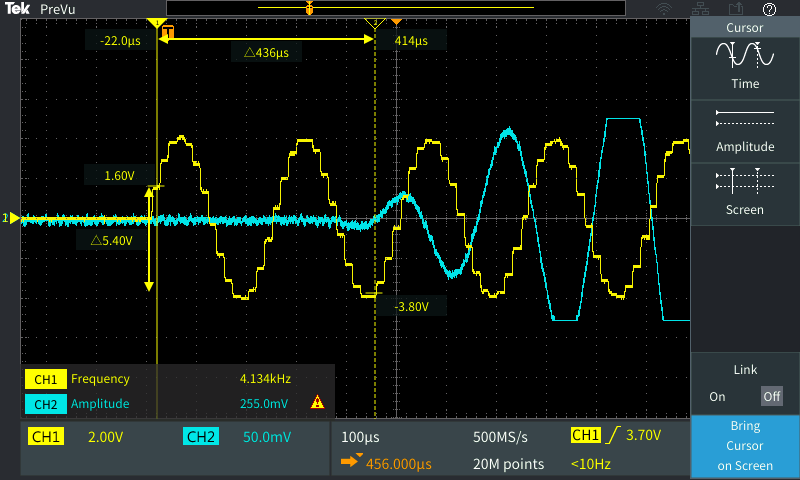
\includegraphics[width=0.8\linewidth]{./images/us_delay_scope.png}
      \caption{Capture of the measurement of ultrasonic delay on the oscilloscope}
      \label{fig:us_delay_scope}
    \end{figure}

  \subsection{Measuring Frequency Response} \label{section:frequency_response}

    After testing for delays, we also measured the frequency response of the NTX-1004PZ piezo speaker. We placed two speakers 17 feet apart, and using a function generator we transmitted a square wave at 8vPP and swept from \SI{20}{\kilo\hertz} to \SI{30}{\kilo\hertz} and back down over the course of 20 seconds. We attached an oscilloscope to the receiving speaker and captured the power at each frequency using the FFT mode, persisting the display over the course of the sweep to see how the frequency response changes across our frequency range. Figure \ref{fig:frequency_response} shows the results of this experiment. From this experiment, we learned that the best frequency response is achieved at \SI{22}{\kilo\hertz}, and the after \SI{27}{\kilo\hertz} the signal is indistinguishable from the noise.

    \begin{figure}[H]
      \centering
      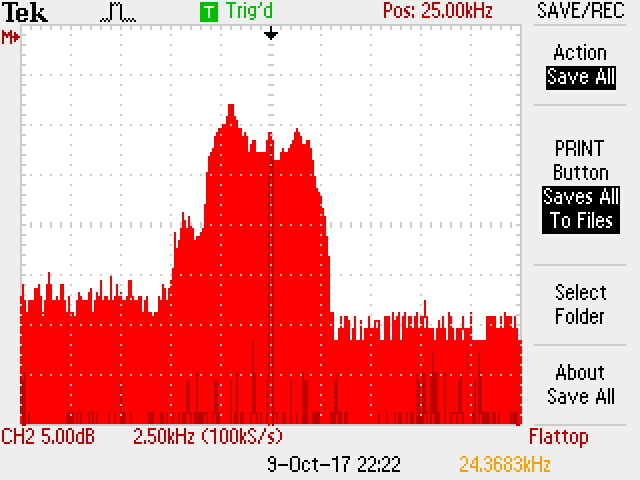
\includegraphics[width=0.7\linewidth]{./images/frequency_response.JPG}
      \caption{Frequency response of the NTX-1004PZ, centered at \SI{25}{\kilo\hertz} with \SI{2.5}{\kilo\hertz} per division. The best response is achieved at \SI{23}{\kilo\hertz}, and the highest detectable frequency is \SI{27.5}{\kilo\hertz}.}
      \label{fig:frequency_response}
    \end{figure}

    This experiment shows that any ultrasonic signals emitted by the beacons must be within the 20-27\SI{}{\kilo\hertz} range. For fixed frequency signals, \SI{22}{\kilo\hertz} should be used. Lower frequencies will be detectable and painful or annoying to humans, and higher frequencies will be undetectable.

  \subsection{A Theoretical Procedure for Building a Map of Beacons} \label{section:beacon_self_localization}

    In order to use beacons to localize, the absolute positions of the beacons must be known. Naively, one could simply place the beacons in fixed locations and measure the position with respect to the field or practice space. However, this is an unsatisfactory solution for our use case in high-speed multi-robot gameplay. It is inevitable that collisions with robots or people working in the space will bump the beacons and change their position. Furthermore, we found in our survey that some FRC teams use a classroom as their practice space, and therefore are unable to leave beacons out in the same position for extended periods of time. Therefore, we describes a procedure by which the beacons, upon initial setup, can discover their own relative positions.

    Consider a ``Cricket'' style beacon using radio and ultrasonic communication like those described in section \ref{section:beacons_background}. Because each beacon is equipped with radio transmitter receiver pair and a piezo transducer, any beacon can send and receive radio signals or ultrasonic chirps to or from any other beacon. This is the principle we will use to construct a map of beacons. The mapping procedure occurs upon startup of the system, or possibly periodically whenever the user believes a new map should be build. We also designate a ``Master'' beacon, which is simply the first beacon that is turned on. The list below outlines the steps required:

    \begin{enumerate}
      \item Identification \\
        \begin{enumerate}
          \item Turn first beacon on, which becomes the master
          \item The master will begin to broadcast itself with a radio message
          \item Turn each other beacon on. Each beacon will hear the master's broadcast message and broadcast a request a Id assignment
          \item The master will hand out sequential Ids to each beacon
          \item After all the beacons have been assign, the identification stage is complete
        \end{enumerate}
      \item Range Data Collection \\
        \begin{enumerate}
          \item The leader starts emitting orders to beacons to send ultrasonic (US) signals to locate the other beacons
          \item When beacon hears its signal, it will chirp US
          \item Everyone else will listen for that US and compute their distance to beacon 1
          \item Then beacon two will hear its signal, and will chirp US
          \item Everyone else will listen and compute distance to beacon 2
          \item Repeat for all the identified beacons
        \end{enumerate}
      \item Map Construction \\
        \begin{enumerate}
          \item At this point, all of the beacons have computed all of the ranges to all other beacons
          \item The master will then one-by-one request each beacon to emit this information
          \item Once the master has collected all range estimates, it uses a least-squares solver to find the distances that minimize the error from all the range estimates
        \end{enumerate}
    \end{enumerate}

    The final step in this procedure is a simple optimization step. The problem can be stated formally as such. Let there be $N$ beacons, let $d_{ij}$ be the true distance from beacon $i$ to $j$, and let $\hat{d}^k_{ij}$ by the distance from $i$ to $j$ as measured by beacon $k$. The optimization problem is as follows:

    \begin{equation} \label{eq:beacon_optimization}
      \argmin_{d_{ij}}\sum_{k=0}^N{\lVert d_{ij}-\hat{d}^k_{ij} \rVert}^2
    \end{equation}

    Because we formulate the optimization problem as a sum of square error, there are many potential optimization methods that could be used, such as Levenburg-Marquedt. The end result will be a set of distances from each beacon to each other beacon. From this point, one can either assume that a given beacon (sensibly beacon 0) is the origin, or one can provide the position of the origin beacon with respect to some other origin on the field of practice space. Either way, this setup procedure and optimization problem result in a map which can be used to find the position of the robot give any collection of measured ranges to three or more beacons.

	\subsection{OpenCV Optical Flow Sample Code}

    Preliminary testing with optical flow was done using a Microsoft USB camera using the sample code provided in OpenCV. In the screenshot below the window labeled flow that there are a variety of green dots on the screen. These are the points that dense optical flow has identified. There is also a green line which is the motion vector of which way the frames are moving. The middle window labeled HSV flow is adding color to the different points that are currently the best for tracking on the frame. The bottom window labeled glitch is the current frame and previous ones overlaid showing all of the motion that has happened.

    \begin{figure}[H]
      \centering
      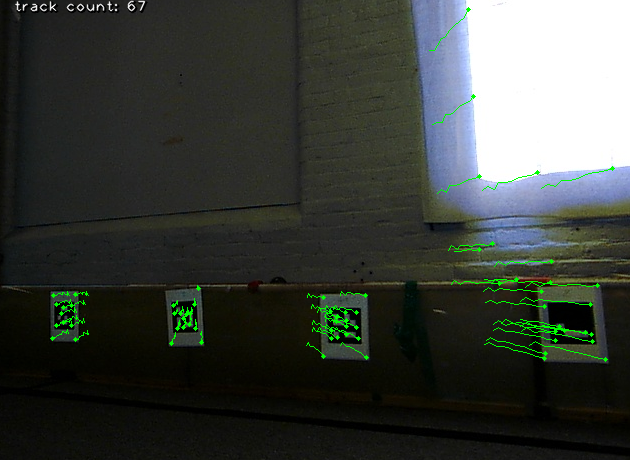
\includegraphics[width=0.49\linewidth]{./images/optflow.png}
      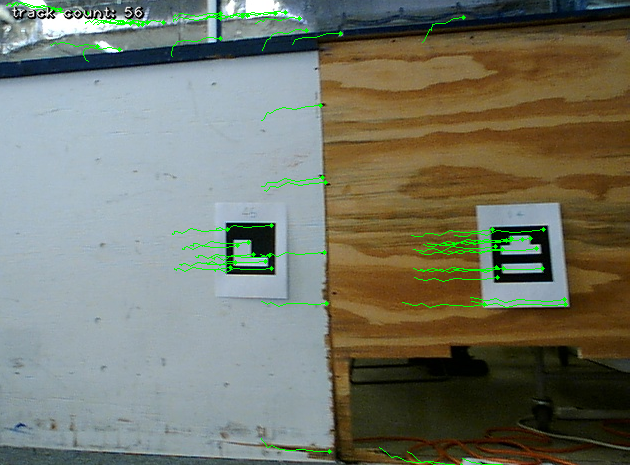
\includegraphics[width=0.49\linewidth]{./images/optflow_2.png}
      \caption{Screenshot of the opencv sample program \texttt{lk\_track.py} on video collected on a practice FRC field. Aruco tags provide excellent targets for Lucas-Kanade tracking.}
      \label{fig:opt_flow}
    \end{figure}

  \subsection{Benchmarking OpenCV Processing Times} \label{section:profiling_opencv}

    This test compares computation time for optical flow with OpenCV. Tests were done using \texttt{lkdemo.cpp} which was we modified from a sample file provided by OpenCV. We compare this program on a laptop verse the RoboRIO and compare the time they took to run the code. The laptop used has a 2.8 GHz Intel 4 Core i7 processor. A chart below was made of the time that each program took to run 100 frames in seconds.

    \begin{table}[H]
      \centering
      \begin{tabular}{l|l|l|}
        \cline{2-3}
        & Laptop (sec) & RoboRIO (sec) \\
        \cline{2-3}
        & 3.638 & 8.429 \\
        & 4.184 & 8.429\\
        & 3.638 & 8.429 \\
        & 3.639 & 8.429 \\
        & 4.184 & 8.429 \\
        \hline
        \multicolumn{1}{|l|}{Average (sec)} & 3.8566 & 8.429 \\
        \multicolumn{1}{|l|}{Average (FPS)} & 26 & 12 \\
        \hline
      \end{tabular}
      \caption{Time for 100 frames to run using OpenCV on laptop verse RoboRIO}
      \label{table:optical_flow_benchmark}
    \end{table}

    We performed these measurements 5 times to ensure repeatability. From these numbers, we conclude the laptop was just over twice as fast that of the RoboRIO. Based on our results from section \ref{section:fps}, we conclude that 12 FPS is not fast enough for our project requirements and so a co-processor is needed.

  \subsection{Collecting Ground-Truth with VICON Motion Capture} \label{section:mocap}

    To evaluate the accurate of our system and to help with tuning various constants in the system we need a source of ground-truth state information. The ground truth data for measuring accuracy and precision is obtained using a VICON brand Motion Capture system. This comprises a VICON Lock+ data processor and 8 Vero infrared cameras. Our system can collect 2.2 megapixels of data and is designed for capturing human motion in small spaces. The VICON system is accurate to approximately \SI{1}{\milli\meter}. In our experiments, the space used for experimentation was 19x14 feet. The pose of the robot is tracked using three retro-reflective markers. These are positioned at known distances such that the transform between the centroid of the markers and the centroid of the robot is easily obtained. A scalene triangle laser cut from acrylic was used as a guide.

    \begin{figure}[H]%
        \centering
        \subfloat[guide for placement]{{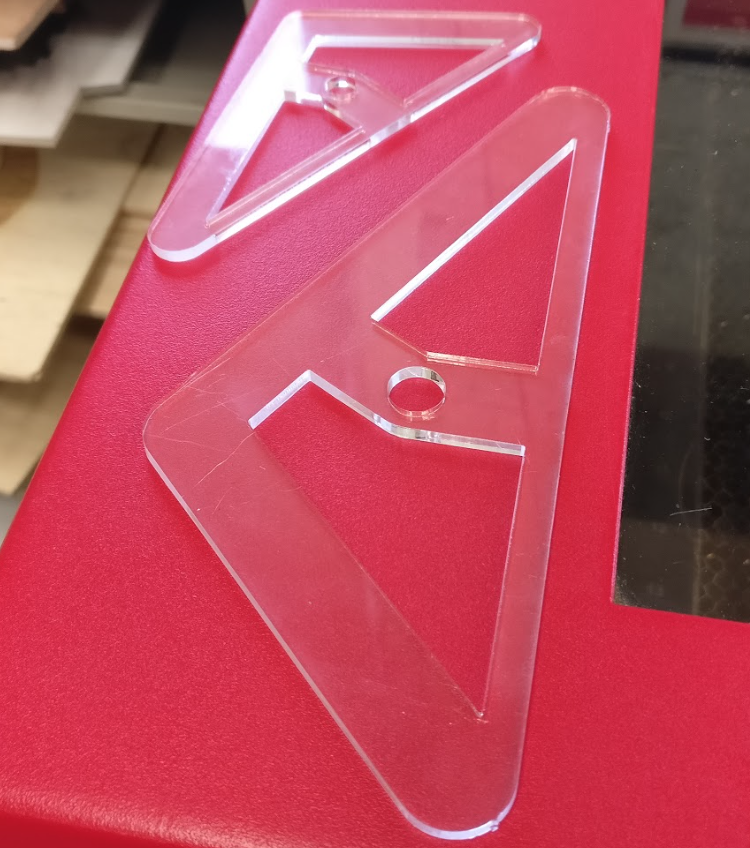
\includegraphics[width=5cm]{./images/calib_triangle.png} }}%
        \qquad
        \subfloat[reflective markers]{{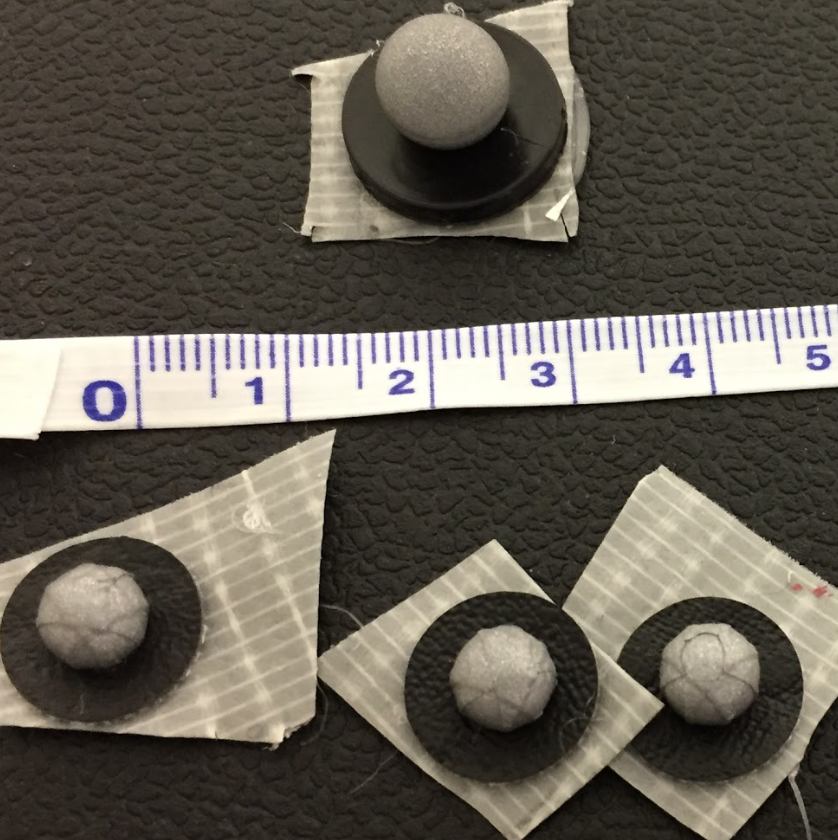
\includegraphics[width=5cm]{./images/vicon_markers.png} }}%
        \caption{VICON tracker set up}%
        \label{fig:viconSetup}%
    \end{figure}

    In our experiments, the camera system captures data at 100Hz. To synchronize data collection, the RoboRIO sends a 5V signal to the Lock+ processor, and a UDP packet is transmitted to the Co-Processor running the camera. This data is synchronous to within $\approx$\SI{500}{\micro\second}. Using the same markers, the pose of the ArUco tags is also measured.

    \begin{figure}[H]%
      \centering
      \subfloat[robot in VICON field]{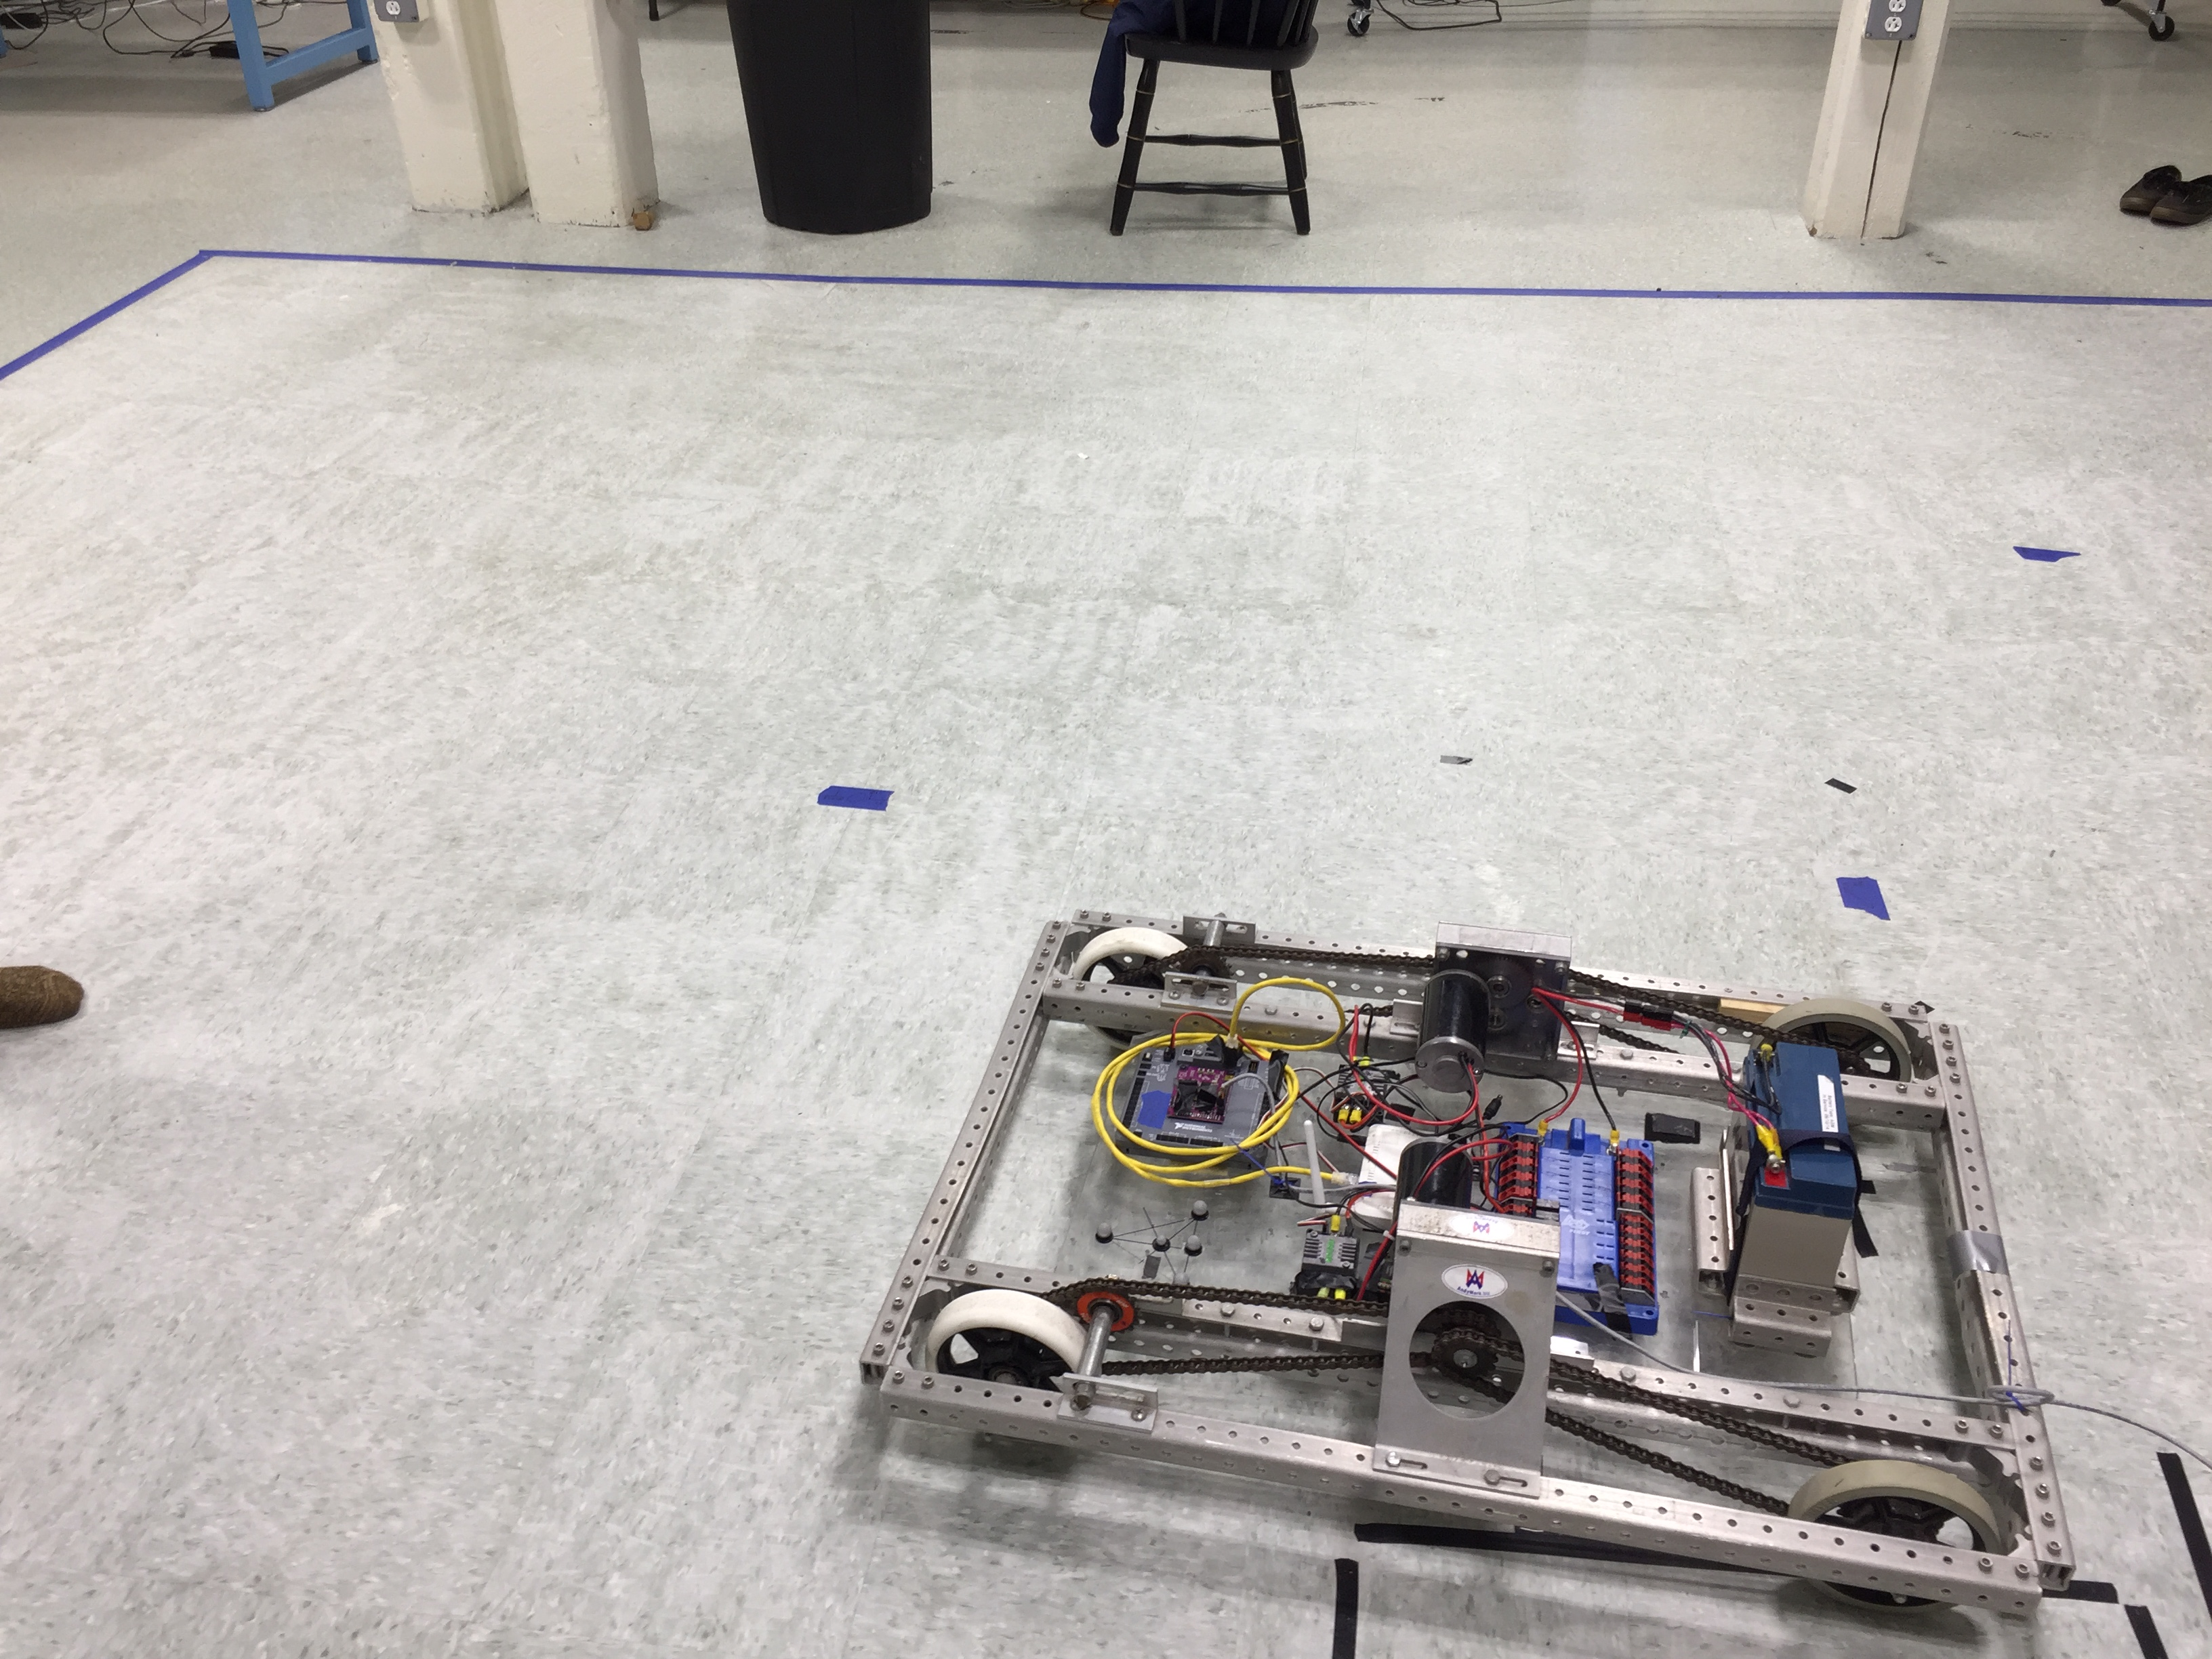
\includegraphics[width=6cm]{./images/robot_in_plane.jpeg}}%
      \qquad
      \subfloat[VICON (blue to red over time) position and orientation data]{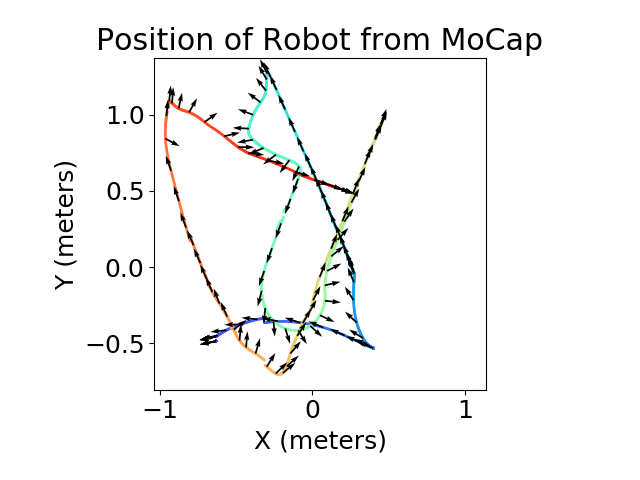
\includegraphics[width=6cm]{./images/example_mocap_1.png}}%
      \caption{Collecting and Plotting Position data}%
      \label{fig:positionData}%
    \end{figure}

    % FIXME redo the results and change out the pictures above now that we have better results

  \subsection{Detecting Simulated Chirps in MATLAB}

    In order to examine the theoretical limits of our ultrasonic chirp detection, we created synthetic chirps and examine how pattern matching filters would work to detect them. For our beacons to work we must be able to very precisely find the start of a chirp given a buffer of ADC readings, and we simulate this in MATLAB. In these experiments, we construct our chirps using matlab's \texttt{chirp} function, and we sweep from 20-27\SI{}{\kilo\hertz} (see section \ref{section:frequency_response} for justification). This signal is shown in figure \ref{fig:unshifted_no_noise_chirp}. The zoomed in version highlights that given a reasonable ADC speed of 108ksps, we will only see a very rough sine wave.

    \begin{figure}[H]
      \centering
      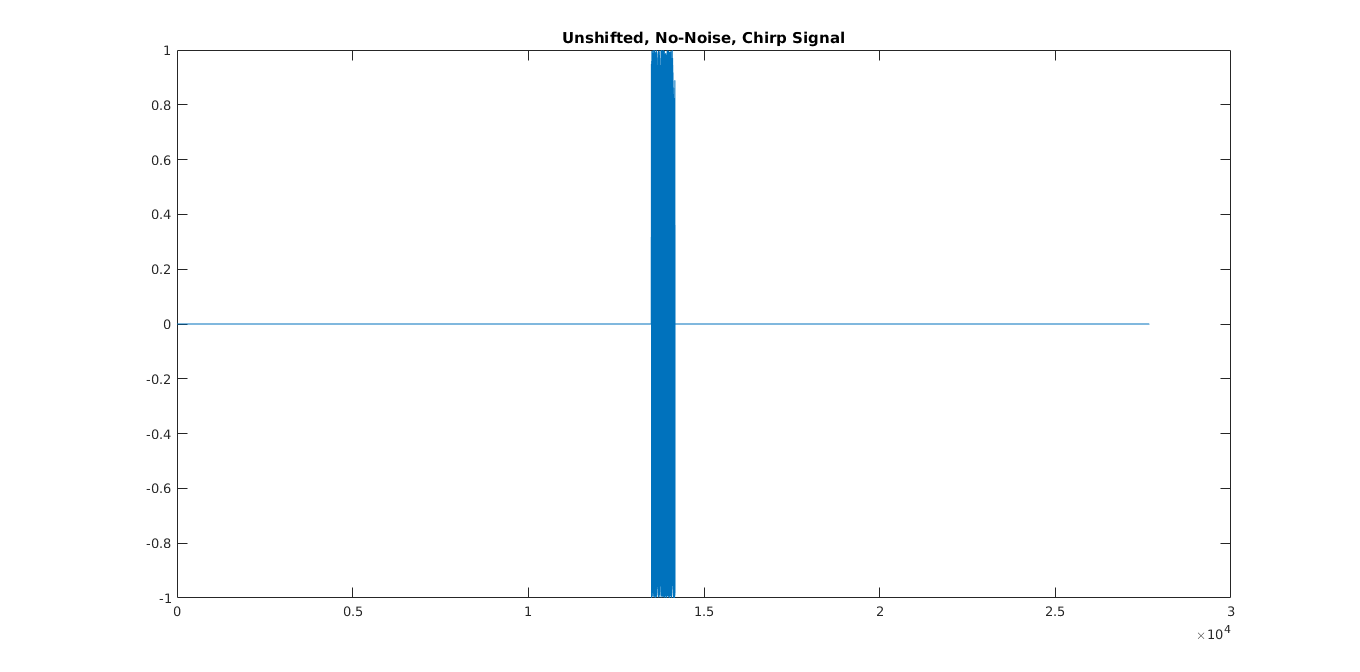
\includegraphics[width=1\linewidth]{./images/unshifted_no_noise_chirp.png}
      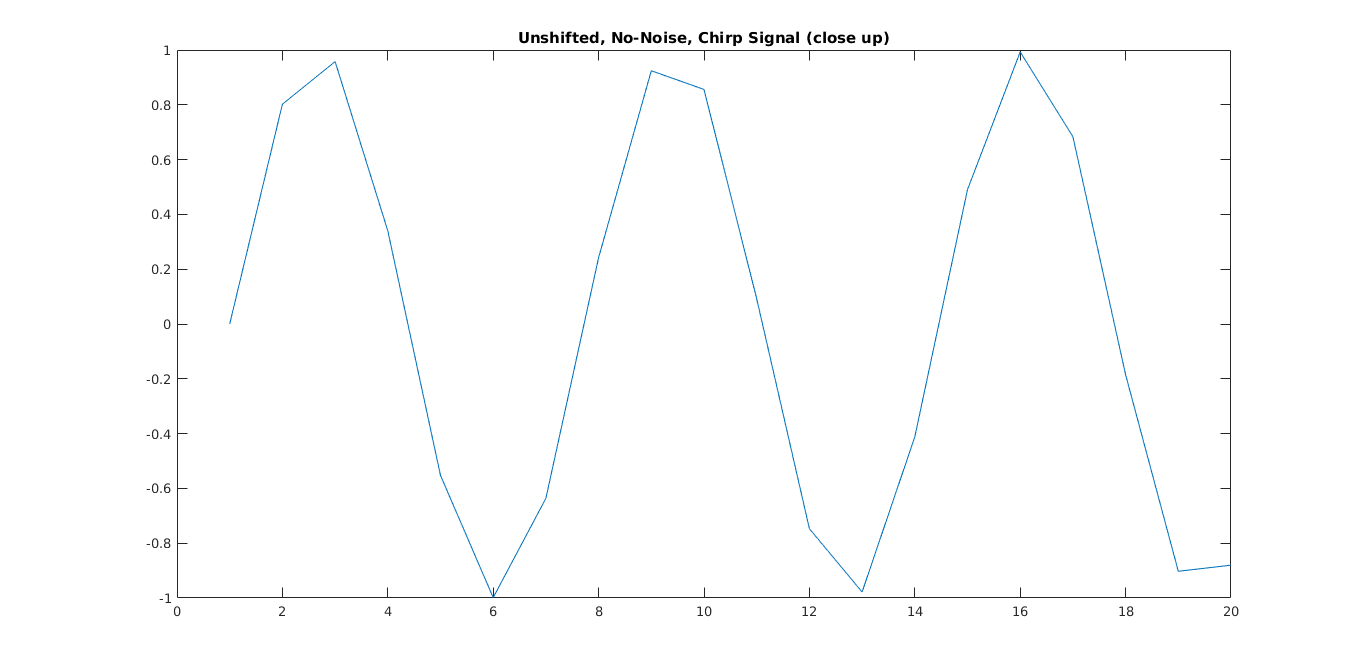
\includegraphics[width=1\linewidth]{./images/unshifted_no_noise_chirp_zoomed.png}
      \caption{Unshifted, No-Noise, Chirp, 20-27\SI{}{\kilo\hertz}}
      \label{fig:unshifted_no_noise_chirp}
    \end{figure}

    Given this original signal, we then pad the signal and add noise. The result of this is shown in figure \ref{fig:repeated_signal}. Finally, use our original clear signal as a pattern, and convolve it with our signal. The result of this is shown in figure \ref{fig:pattern_matching}.

    \begin{figure}
      \centering
      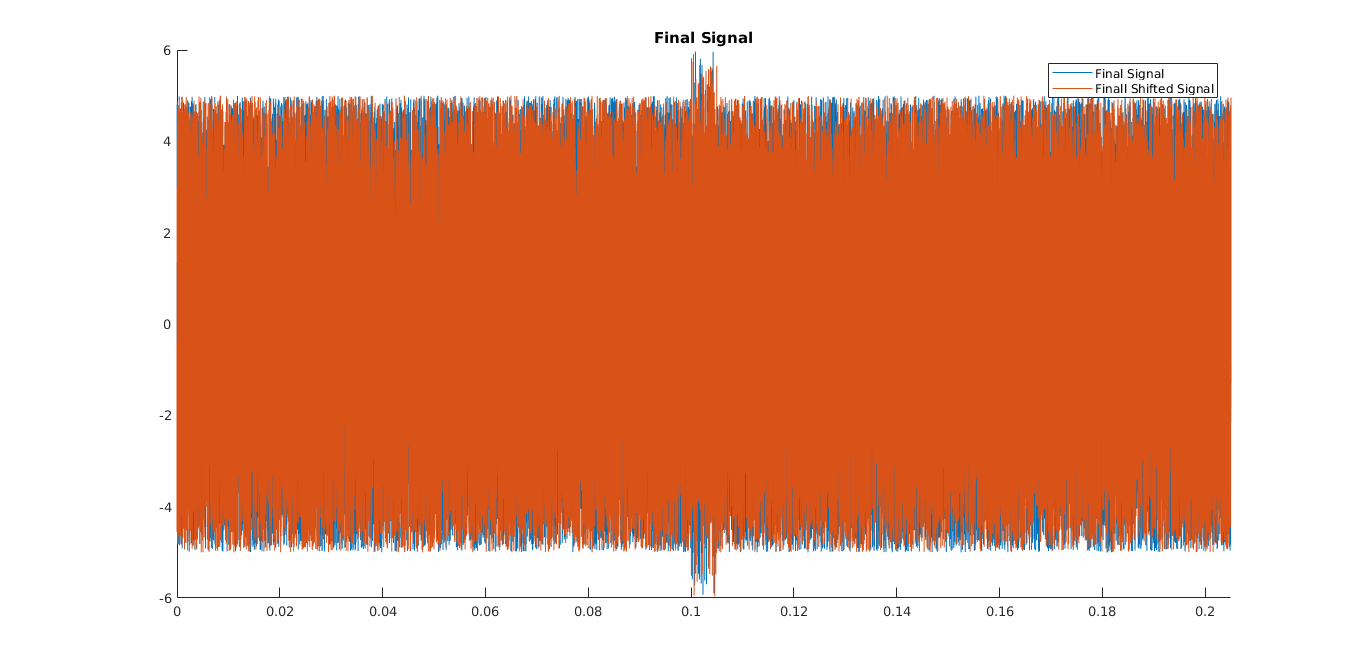
\includegraphics[width=1\linewidth]{./images/repeated_noisy_signal.png}
      \caption{Both the Doppler shifted and unshifted full noisy signals.}
      \label{fig:repeated_signal}
    \end{figure}

    \begin{figure}
      \centering
      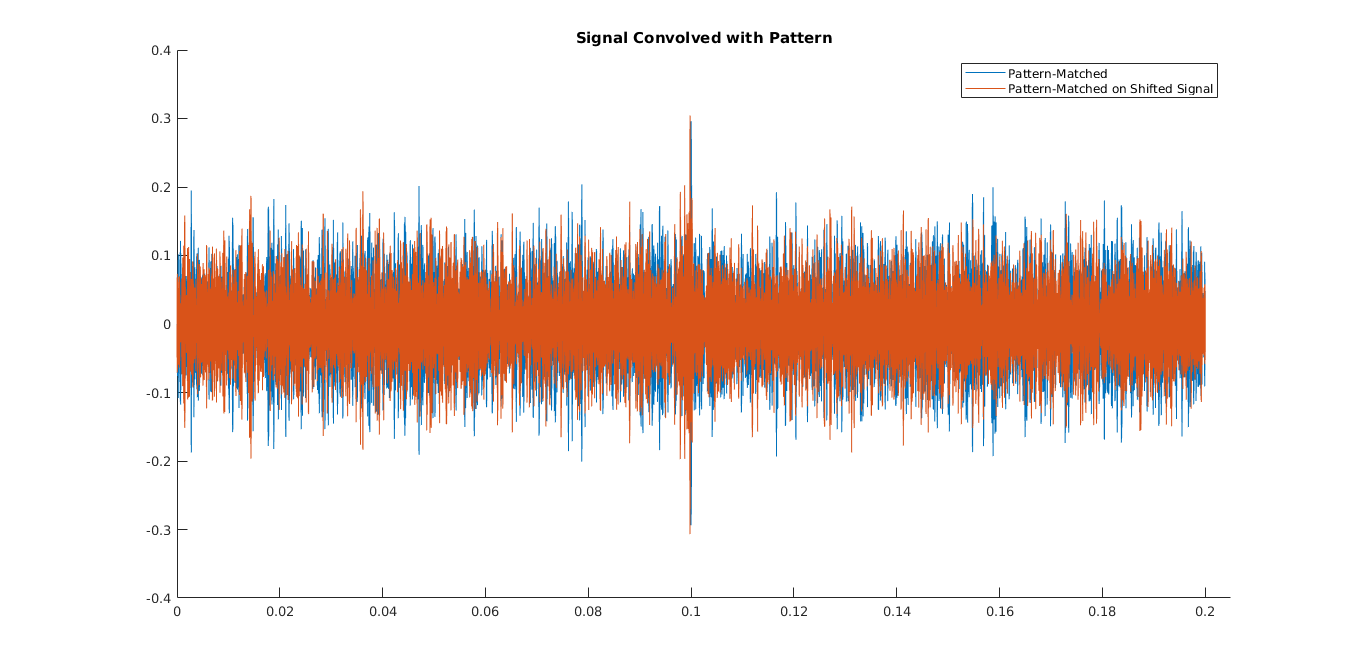
\includegraphics[width=1\linewidth]{./images/pattern_matching.png}
      \caption{The peaks in the center indicate the pattern matching the noisy signals closely.}
      \label{fig:pattern_matching}
    \end{figure}

    \subsubsection{The Doppler Effect on Ultrasonic}

      %TODO review this section. some of it is WRONG

      Using these simulated chirps, we ask the question of whether the Doppler effect of a moving FRC robot will make the signal undetectable with simple pattern matching. The plots above show what happens if a Doppler shift of a robot moving \SI{3}{\meter\per\second} is introduced. This speed causes a Doppler shift of \SI{291.3}{\hertz}, and after applying pattern matching using the unshifted filter we see that the chirp is detected \SI{192.5}{\micro\second} early, which corresponds to \SI{6.6}{\centi\meter} of error, which is within our requirements (see section \ref{section:defining_success}). Furthermore, when the Doppler has no effect, the error of our simulated detection is just \SI{2.5}{\milli\meter}, which is well within our requirements.

    \subsubsection{Effect of Chirp Bandwidth}

      One of the main limiting factors of using cheap piezo speakers is the limited range of frequencies that induce a measurable response (see \ref{section:frequency_response}. Using our simulated chirps, we experimented with changing the frequency range over which the chirps sweep. When we use the full range of 20-27\SI{}{\kilo\hertz}, the amplitude of the match filter is higher and the error is lower. However, when a smaller range such as 23-24\SI{}{\kilo\hertz} is used, the amplitude of the match filter is lower, and more difficult to distinguish with a simple threshold. For the implementation of a beacon system, this means that the chirps should span as wide a frequency range as possible.


    %The VDAC8 on the psoc 5LP is limited by its speed setting options. There are only two options for what speed the DAC can be set to which are slow and high. The datasheet says that the slow option makes the settling time slower but consumes less operating current and the high mode does the opposite. The datasheet provides no further information about these settings so there is not a provided way to know the speed of the DAC. The DAC also is only 8 bit it can only be set to values between 0 and 255 which has not yet been a problem but is a limiting factor in general.
    %The Delta Sigma ADC has a resolution range of 8-20 bits.The lower the resolution the larger the range for conversion rate in samples per second. But even with the lowest resolution of 8 bits the range is only 8000-192000 which limits the minimum and maximum sample rate that can be used.

  \subsection{Ultrasonic Beam Spread}

    % could at do beam-spread equation here
    If we model our piezo speakers as flat piston transducers, then we can derive the beam divergence angle as follows \cite{bond_beam_2001}. $V$ is the speed of sound, $D$ is the diameter of the transducer, and $F$ is the frequency.

    \begin{align} \label{eq:beam_divergence}
      \begin{split}
        \sin(\theta) &= 1.2\frac{V}{DF} \\
        \theta &= \sin^{-1}\bigg(1.2\frac{343}{0.0381*25000}\bigg) \\
        \theta &= 0.44684 = \ang{25.6}
      \end{split}
    \end{align}

    Therefore, the total beam angle of these speakers is theoretically \ang{51.2}. Verifying this experimentally is left for future work, however this theoretical number can be used to estimate the number of beacons needed to give full coverage of the practice space in which the robot is operating.

  \subsection{Characteristics of Piezo Transducers}

    Throughout this project we also discovered several interesting characteristics of our piezo speakers. First, we note that emitting square versus sine waves does not seem to effect the received signal, given the same amplitude and frequency. We tested this by connecting on piezo to a function generator and another to an oscilloscope. We generated a high frequency wave, toggling between either square or sine wave, and compared the received waveform on the oscilloscope. By simply looking at the waveform, we were unable to determine whether the function generator was in square or sine wave mode. This means that even if the transmitting speaker is being moved like a square wave, the receiving transducer will simply resonate at the same frequency and the received signal will be a sinusoidal wave. This impacts implementation because square waves can be produced with high-precision digital components rather than analog components like DACs, so one may choose to use a square wave instead of a sine wave.

	\subsection{Co-Processors for Image Processing}

    Since our system requires processing of images from a video stream, we evaluated the Raspberry Pi 3 and the NVidia TK1 as potential co-processors. We ruled out the RoboRIO for image processing because many teams in FRC have found the RoboRIO insufficient for vision processing, and because we did not intend for computational efficiency to be a key criteria of this project. Further still, using a coprocessor allows us to write and run whatever our system requires, irrespective of how any teams actual robot code is operating.

    % FIXME: More testing here. How high FPS/resolution can we get on each platform?

  \subsection{Evaluting The Placement of ArUco Tags} \label{section:tag_placement}

    When doing localization with ArUco markers, generally the more markers that can be detected the better your pose estimates and maps will be. However, this is also a trade off with the amount of modification required in the environment. We would like to have as few tags as possible in our environment to minimize the amount of work required to localize in that environment. To begin to answer this question, we consider how the spacing between tags on a mock FRC field effects the detection rate of tags.

    \begin{figure}[H]
      \centering
      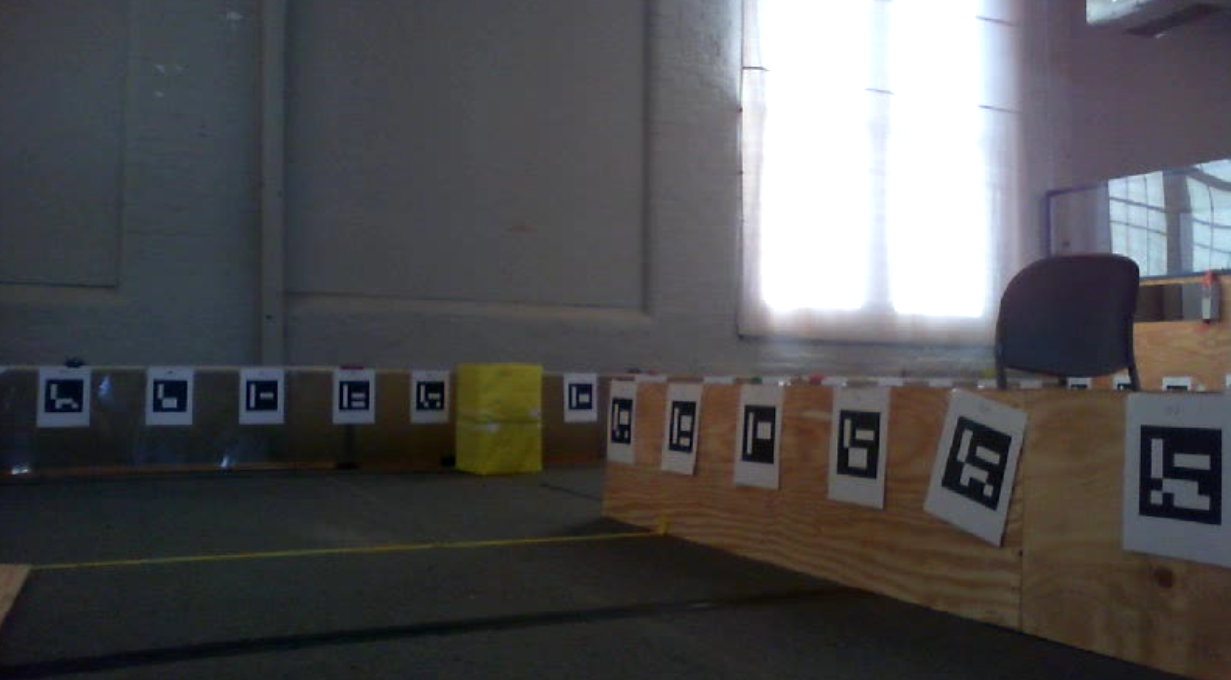
\includegraphics[width=1\linewidth]{./images/nypro_tag_spacing.png}
      \caption{Tags placed on the Nypro practice field}
      \label{fig:nypro_tag_spacing}
    \end{figure}

    We placed \SI{0.152}{\meter} tags every 1.5ft on a mock FRC field at Nypro (see Figure \ref{fig:nypro_tag_spacing}). We recorded video driving realistically around the field and counted how frequently we detected ArUco tags. We then filtered out tags by their ID numbers to simulate spacings of 3ft, 4.5ft, and 6ft. We report detection statistics for each of these spacings based on two different runs through the field in Table \ref{table:spacing_timing}. We also plot all the times between detections over the course of one of our runs in Figure \ref{fig:spacing_timing}. Our results show that, assuming reasonable camera settings of 480p30 (640x480, 30fps), the frequency of tag detection is essentially unchanged between 1.5ft and 6ft spacings. The only notable difference is the mean time between detections slowly rises as tags become further apart. Intuitively, this means that even 6ft between tags is close enough to expect to detect tags 10 times a second. More specifically, we can say that 95\% of the time we will detect a tag every \SI{0.1}{\second}. We do note that during our first trial, where our camera was accidentally only recording frames at 480p8, the tag detection rate suffers more significantly as tag detection increases.

    \begin{table}[H]
      \centering
      \begin{tabular}{|c|c|c|c|c|c|c|c|c|} \hline
        spacing (ft) & \multicolumn{2}{c}{worst case (s)} & \multicolumn{2}{c}{95th percentile (s)} & \multicolumn{2}{c}{mean (s)} & \multicolumn{2}{c|}{median (s)} \\ \hline
            & trial 1 & \textbf{trial 2} & trial 1 & \textbf{trial 2} & trial 1 & \textbf{trial 2} & trial 1 & \textbf{trial 2} \\ \hline
        1.5 & 5.100 & \textbf{3.700} & 0.762 & \textbf{0.068} & 0.235 & \textbf{0.053} & 0.132 & \textbf{0.032} \\ \hline
        3.0 & 5.231 & \textbf{3.700} & 0.932 & \textbf{0.100} & 0.269 & \textbf{0.061} & 0.132 & \textbf{0.032} \\ \hline
        4.5 & 5.900 & \textbf{3.700} & 1.145 & \textbf{0.100} & 0.284 & \textbf{0.064} & 0.132 & \textbf{0.032} \\ \hline
        6.0 & 7.832 & \textbf{3.700} & 1.343 & \textbf{0.100} & 0.335 & \textbf{0.070} & 0.132 & \textbf{0.032} \\ \hline
      \end{tabular}
      \caption{Tag detection metrics compared across tag spacings.
      The larger spacings have slightly worse performance, but still usually provide updates at least 10 timers per second.
      Trial 1 only recorded at 8fps, but is included for completeness. Trial 2 was 30fps.}
      \label{table:spacing_timing}
    \end{table}

    \begin{figure}[H]
      \centering
      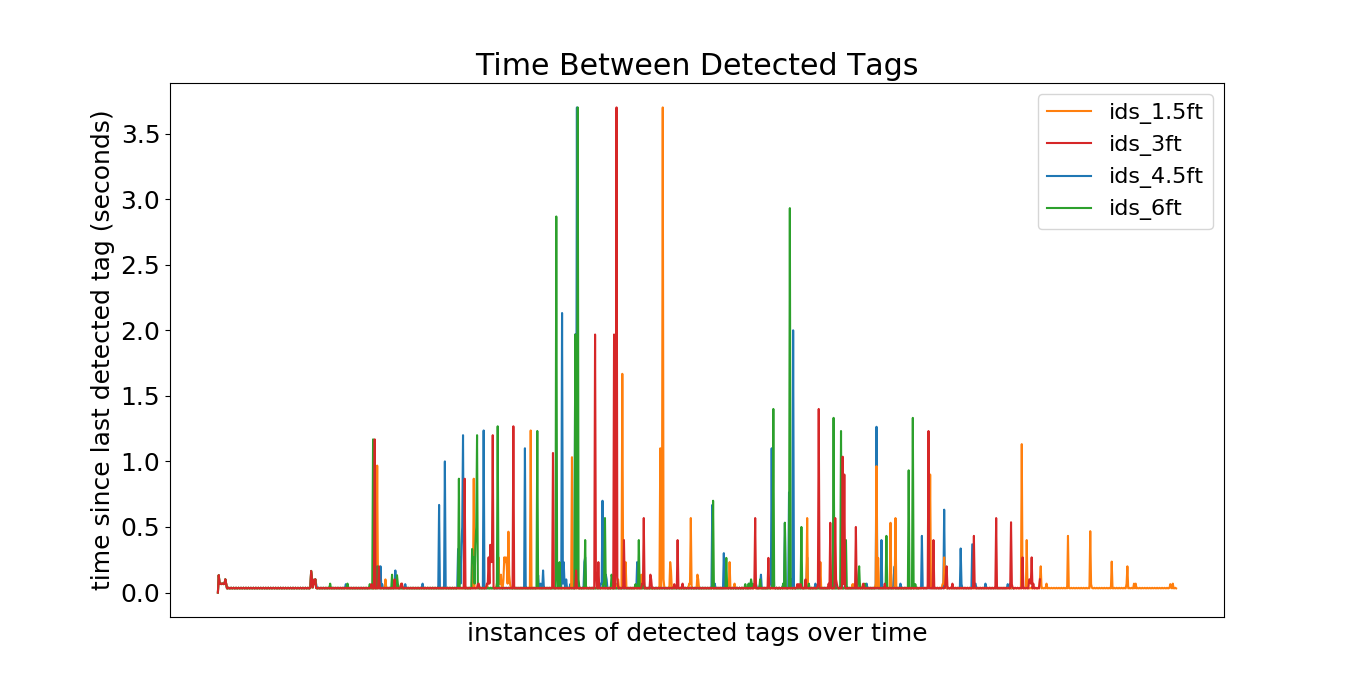
\includegraphics[width=1\linewidth]{./images/spacing_times.png}
      \caption{Times between detected tags as a function of tag spacing. Spacings between 1.5ft and 6ft perform very similarly.}
      \label{fig:spacing_timing}
    \end{figure}


    It is important to note several other factors that are not explored here, including how spacing and positioning effects the accuracy of detections. Furthermore, one should ask whether the specific locations of tags, not just the spacing between them, also effects detection accuracy and frequency. Intuitively, we claim that tags should be placed in locations where the robots camera is likely to be facing, such as feeding stations and goals. However, we do not empirically evaluate this claim.

	\subsection{Statistics of CSCore Image Timestamps}

    We use the built-in API of CSCore (\url{https://github.com/wpilibsuite/cscore}) to get the time stamps (in microseconds) for each image captured. During many of our tests, we logged these times to files for offline processing. We now ask how much these time stamps vary from the requested FPS. This is important information to know, because it effects whether or not one can assume a truly constant FPS. We find that there is significant variation between any individual frames. Table \ref{table:fps_stats} shows key statistics about FPS over a multitude of recordings from our test robot. These recordings are taken from our tests at Nypro, with various requested frame rates and at various resolutions.

    \begin{table}[H]
      \centering
      \begin{tabular}{|c|c|c|c|c|c|} \hline
        Requested FPS & Resolution & Mean FPS & Median FPS & Min FPS & Max FPS \\ \hline
        30 & 1920x1080 & 14.90 & 14.71 & 9.61 & 22.75 \\ \hline
        30 & 1920x1080 & 15.11 & 14.71 & 10.00 & 27.83 \\ \hline
        30 & 1280x720 & 8.17 & 7.59 & 2.29 & 14.78 \\ \hline
        30 & 1280x720 & 8.35 & 7.60 & 2.00 & 14.75 \\ \hline
        30 & 800x448 & 29.34 & 31.08  & 4.31 & 31.78 \\ \hline
        60 & 640x480 & 59.43 & 60.02 & 3.53 & 62.48 \\ \hline
        60 & 640x480 & 59.71 & 60.02 & 3.33 & 89.32 \\ \hline
        30 & 640x480 & 30.00 & 30.01 & 3.76 & 30.13 \\ \hline
        30 & 320x240 & 30.04 & 31.21 & 2.72 & 31.71 \\ \hline
        30 & 320x240 & 30.03 & 31.22 & 3.33 & 32.30 \\ \hline
        30 & 320x240 & 30.08 & 31.21 & 14.76 & 32.69 \\ \hline
      \end{tabular}
      \caption{Table of statics from a multitude of CSCore streams. We find that FPS can vary throughout normal operation.}
      \label{table:fps_stats}
    \end{table}

    We observe that startup-lag is the true cause of low minimum FPS, and therefore does not cause significant issues unless pose estimates from the first two frames are critical. However, there are in fact cases where the camera exceeds the desired FPS but as much as 48\% in the case of 60fps. There are also several cases where the processing collecting and stamping these images was not powerful enough to acheive the requested FPS. For example, we requested 720p30 on a Raspberry Pi, but were only able to capture at $\approx$15fps. This is real constraint that must be handled in a camera based localization system, and so we report those results for completeness. However, our results show that, assuming the computer is powerful enough to acheive the requested FPS on average, there are only small variations on FPS over time. We provide two full plots of FPS over time in two of the more curious entries in table \ref{table:fps_stats} to be more illistrative of how time between frames can vary (figures \ref{fig:fps_plot_1} and \ref{fig:fps_plot_2}).

    \begin{figure}[H]
      \centering
      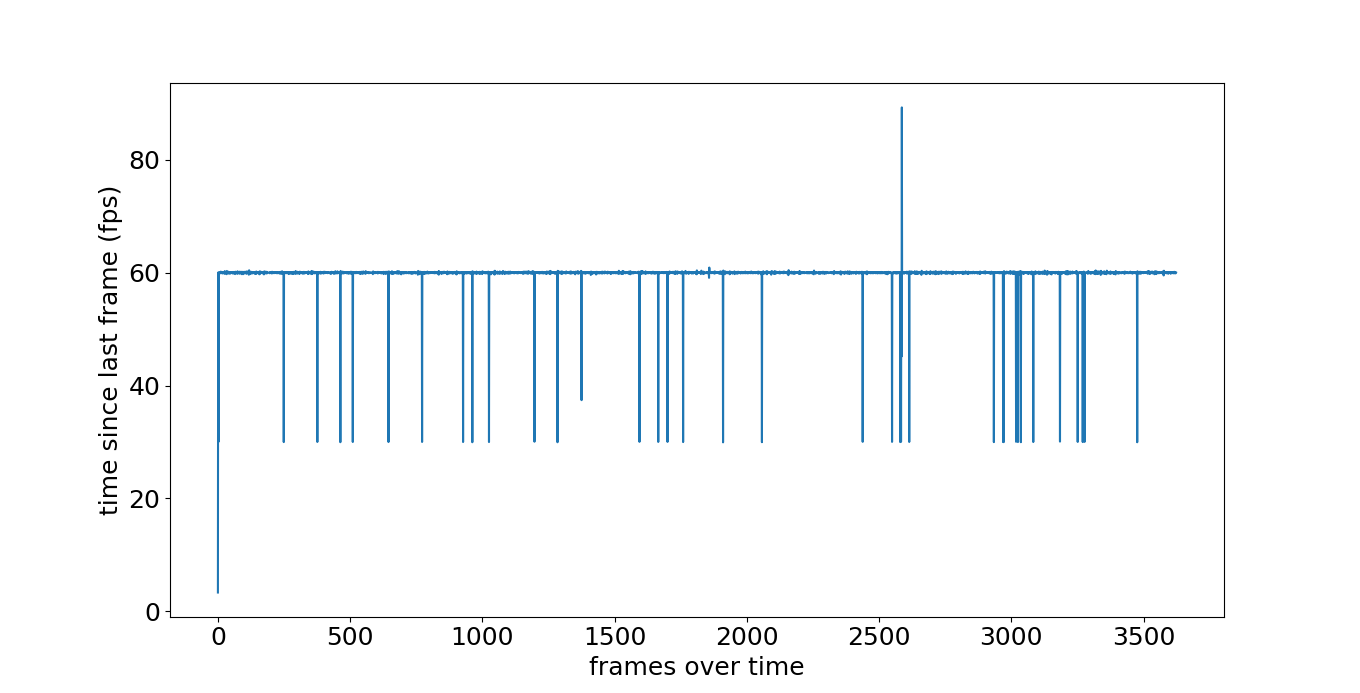
\includegraphics[width=0.8\linewidth]{./images/fps_plot_2.png}
      \caption{FPS over time for one instance of 240p30}
      \label{fig:fps_plot_2}
    \end{figure}

    \begin{figure}[H]
      \centering
      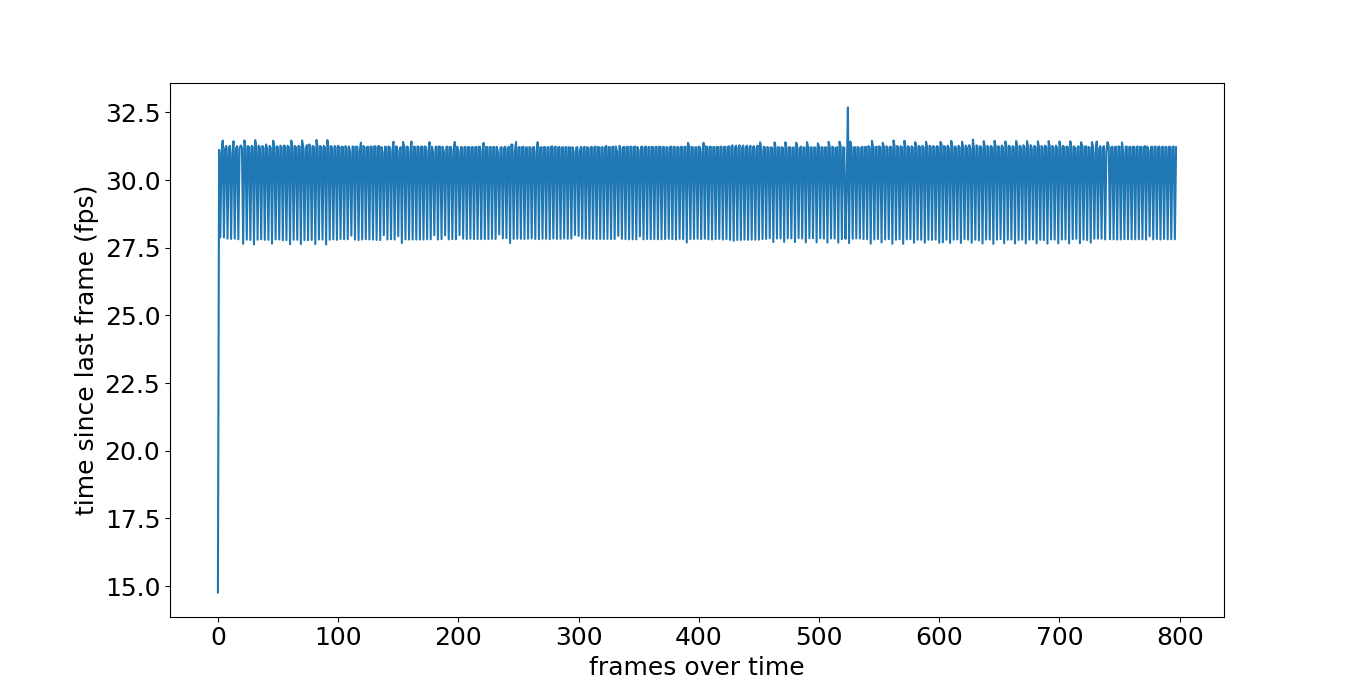
\includegraphics[width=0.8\linewidth]{./images/fps_plot_1.png}
      \caption{FPS over time for one instance of  480p60}
      \label{fig:fps_plot_1}
    \end{figure}

  \subsection{Effect of Frame Rate and Resolution on ArUco Tag Detection} \label{section:fps}

    We explore the effect of frame rate and resolution on the frequency with which tags are detected. This frequency of detected tags is an important metric because it sets the standard for how long our dead-reckoning methods must run without receiving an update to compensate for drift. Furthermore, since the FPS and resolution of a camera correlates with cost, we want to know whether a cheap camera is sufficient for tag detection.

    To answer this question, we used three cameras simultaneously recording footage from the robot as we drove around a mock FRC Field. It is important that these cameras are recording simultaneously and are mounted right next to each other, because it means the camera streams will see essentially the same view of the world, with the only variable being the resolution and FPS. The tags were placed roughly every 6 feet (according to results of section \ref{section:tag_placement}) and the robot was driven through a simulated FRC game for \SI{60}{\second}. We then compare how frequently tags were detected by looking at gaps between detections. Table \ref{table:tag_detection_comparison} shows a comparison of various key metrics between the different resolution/FPS pairings. The full plots showing all gaps in the run is shown in appendix \ref{appendix:tag_detection}

    \begin{table}[H]
      \centering
      \begin{tabular}{|c|c|c|c|c|c|} \hline
        Condition & Worst-Case (s) & 95th percentile (s) & Mean (s) & Median (s) & Mode (s) \\ \hline
        PS3 Eye 480p30 & 4.565 & 0.100 & 0.062 & 0.033 & 0.033 \\ \hline
        PS3 Eye 480p60 & \textbf{3.049} & \textbf{0.033} & \textbf{0.032} & \textbf{0.017} & \textbf{0.017} \\ \hline
        C920 1080p15 & 3.196 & 0.767 & 0.162 & 0.068 & 0.068 \\ \hline
      \end{tabular}
      \caption{480p30 means 640x480 at 30fps, 480p60 means 640x480 at 60fps, 1080p15 means 1920x1080 at 15fps. The best settings by all measures was the PS3Eye camera at 60fps.}
      \label{table:tag_detection_comparison}
    \end{table}

    Arguably the most important metric here is the 9th percentile metric, which says that 95\% of of the time gaps between detected tags are less than that number. Generally, that number is quite close to the mean frame rate which means that usually you get one tag detected in every frame, but this is of course not always true. It's important to note that just because a there was a tag detected in the frame doesn't mean we get a reliable position estimate from that tag. So these numbers are not the same as the how frequently an actual position is received, which is what we truly care about.

    In conclusion, the 480p60 setting performs the best by all metrics, and therefore we recommend using those settings.

  \subsection{Rate of position estimates from ArUco Tags}

    Although the detection of tags, is important, what is really important is the estimates of their pose. We now consider only valid position estimates, and not just any detected tag, and measure the frequency of pose estimates from our camera. We use the same recordings at the Nypro test field as we have used throughout this report, and similar to section \ref{section:tag_placement} we compare the time between valid pose estimates. For completeness, we also compare this across the three resolution/fps settings which were recorded. One notable oddity in the data is the extremely high variance in the worst-case time between pose detections across trials and tag spacings. We simulated tag-spacings by filtering out tags based on their IDs, which is accurate because tags were placed in order. However, it means that it's possible for a tag that is present in more sparsely spaced group (ex: 6ft) to be missing from densely spaced group (4.5ft). We can explain this high variance by saying that there was a tag included in the 6ft spacing test that was not present in the 4.5ft spacing test, and without that tag there is a longer period in which no tags are seen. Secondly, we can also say that the high variance between the two trials is explained by the different paths the robot took in each trial. This is a very important result, because it means that depending on how a robot moves through the field, the frequency of valid pose estimates will change.

    \begin{table}[H]
      \centering
      \begin{tabular}{|c|c|c|c|c|c|c|c|c|} \hline
        spacing (ft) & \multicolumn{2}{c}{worst case (s)} & \multicolumn{2}{c}{95th percentile (s)} & \multicolumn{2}{c}{mean (s)} & \multicolumn{2}{c|}{median (s)} \\ \hline
            & trial 1 & trial 2 & trial 1 & trial 2 & trial 1 & trial 2 & trial 1 & trial 2 \\ \hline
            1.5ft & 2.7960 & 3.1961 & 0.2420 & 0.7736 & 0.1135 & 0.1623 & 0.0680 & 0.0680 \\ \hline
            3ft   & 3.5960 & 4.0040 & 0.9228 & 0.9680 & 0.1804 & 0.1958 & 0.0680 & 0.0680 \\ \hline
            4.5ft & 6.5961 & 6.4640 & 1.0160 & 1.2224 & 0.2316 & 0.2556 & 0.0680 & 0.0680 \\ \hline
            6ft   & 10.7960 & 4.7259 & 0.8038 & 1.1300 & 0.2703 & 0.2625 & 0.0680 & 0.0680 \\ \hline
      \end{tabular}
      \caption{Statistics of Pose Estimates from two trials of 1080p15 footage, across various tag spacings. Note the high variance in worst-case across.}
      \label{table:1080p15_pose_estimate_stats}
    \end{table}

    \begin{table}[H]
      \centering
      \begin{tabular}{|c|c|c|c|c|c|c|c|c|} \hline
        spacing (ft) & \multicolumn{2}{c}{worst case (s)} & \multicolumn{2}{c}{95th percentile (s)} & \multicolumn{2}{c}{mean (s)} & \multicolumn{2}{c|}{median (s)} \\ \hline
            & trial 1 & trial 2 & trial 1 & trial 2 & trial 1 & trial 2 & trial 1 & trial 2 \\ \hline
        1.5ft & 1.5161 & 3.0489 & 0.0334 & 0.0334 & 0.0295 & 0.0324 & 0.0167 & 0.0167 \\ \hline
        3ft   & 1.5161 & 5.8312 & 0.0500 & 0.0334 & 0.0437 & 0.0448 & 0.0167 & 0.0167 \\ \hline
        4.5ft & 2.9823 & 7.2807 & 0.0333 & 0.0333 & 0.0479 & 0.0553 & 0.0167 & 0.0167 \\ \hline
        6ft   & 2.2492 & 6.9642 & 0.0334 & 0.0334 & 0.0445 & 0.0533 & 0.0167 & 0.0167 \\ \hline
      \end{tabular}
      \caption{Statistics of Pose Estimates from two trials of 480p60 footage, across various tag spacings.}
      \label{table:480p60_pose_estimate_stats}
    \end{table}

    \begin{table}[H]
      \centering
      \begin{tabular}{|c|c|c|c|c|c|c|c|c|} \hline
        spacing (ft) & \multicolumn{2}{c}{worst case (s)} & \multicolumn{2}{c}{95th percentile (s)} & \multicolumn{2}{c}{mean (s)} & \multicolumn{2}{c|}{median (s)} \\ \hline
            & trial 1 & trial 2 & trial 1 & trial 2 & trial 1 & trial 2 & trial 1 & trial 2 \\ \hline
        1.5ft & 3.6987 & 4.5651 & 0.0666 & 0.1000 & 0.0517 & 0.0621 & 0.0333 & 0.0333 \\ \hline
        3ft   & 4.8316 & 5.8313 & 0.0667 & 0.1999 & 0.0711 & 0.0899 & 0.0333 & 0.0333 \\ \hline
        4.5ft & 8.1971 & 7.1642 & 0.0766 & 0.1500 & 0.1206 & 0.1104 & 0.0333 & 0.0333 \\ \hline
        6ft   & 10.4296 & 6.8976 & 0.1483 & 0.1517 & 0.1164 & 0.0959 & 0.0333 & 0.0333 \\ \hline
      \end{tabular}
      \caption{Statistics of Pose Estimates from two trials of 480p30 footage, across various tag spacings.}
      \label{table:480p30_pose_estimate_stats}
    \end{table}

    If we consider the 59th percentile metric as our most important metric, we should ask what spacing and resolution/fps settings give acceptably fast update rates. If we desire updates at least every \SI{0.1}{\second} (see section \ref{section:defining_success} for justification), then we say that 480p60 will be sufficient at any of the tested tag spacings. On the other hand, 1080p15 gives update too infrequently no matter how close tags are spaced. This makes sense, because at 15fps, a tag would need a valid pose estimate in essentially every frame to acheive \SI{0.1}{\second} update rate. Lastly, we can say that 480p30 probably would work with 1.5ft and 3ft spacings, and it becomes slightly too slow at 4.5ft and 6ft spacings. Ultimately, we recommend using 480p60, and suggest a 6ft spacing so as to minimize the modification of the environment.

    % also compare position estimates between each of the cameras
    % compare graphically over time
    % compare individual points in frames
    % compare covariance after Kalman filtering

	\subsection{Benchmarking MarkerMapper with VICON Motion Capture}

    In this experiment, we determine how close the poses of markers in MarkerMapper map are to their true poses. We built three markermaps, then compare to the positions of markers according to VICON Motion Capture data. As described in section \ref{section:mocap}, the VICON is very accurate, and so it can serve as a reliable ground truth. We placed dots one the tags where we wanted to track them, and recorded the poses and orientations of each tag. Note that there are many more tags in the markermaps (48) than are tagged with motion capture (12). This is because it is difficult to track many shapes in motion capture with similar geometry, such as the triangle pattern of dots we used on our tags. When too many similar geometries are tracked, they can swap with each other and produced uninterpretable data. Therefore, we track one tag on each ``board'', which each board containing 8 tags. For each of the three maps we made, we then systematically compare the tag positions to the motion capture positions in three ways. First, we look at the translation error between corresponding tags. There are multiple ways to do this, however, because one must choose some common reference point in the motion capture and MarkerMapper frames. Therefore, we first consider the error if we align the MarkerMapper and motion capture estimates of tag 0's pose. With tag 0 aligned, we can compare the translation and rotation error between each of the other tags capture in MarkerMapper and motion capture. Then, we align tag 1, and repeat the same error calculation but now for all the tags except tag 1. Finally, we take the average of this procedure over all the alignments. These average rotational and translational errors are the final error we report for each map. Rotational error is given as the angle between the Z axes and Y axes of the marker. We also provide an additional metric, shown in the first column of Table \ref{table:markermapper_accuracy}. This is the error from each tag to tag 0. To compute this, we go through each tag and compute the distance to tag 0 according to motion capture and according to our map, and compare those values to get an error. The average of these errors over each tag is the ``Error To Tag 0'' metric. This simply provides another perspective on translational errors. Because these errors are consistently lower than the other translational error metric, we can say that MarkerMapper is more accurate at estimating the relative distances between tags than it is at estimating the absolute positions of tags in space. This is unsurprising, since the actual measurements MarkerMapper gets is from transforms between projections of tags in camera frames.

    \begin{table}[H]
      \centering
      \begin{tabular}{|c|c|c|c|} \hline
        Error To Tag 0 (m) & Translational (m) & X Rotation (deg) & Z Rotation (deg) \\ \hline
        0.120 & 0.318 & 10.739 & 8.517 \\ \hline
        0.093 & 0.165 & 10.991 & 4.560 \\ \hline
        0.091 & 0.114 & 1.4660 & 3.803 \\ \hline
      \end{tabular}
      \caption{The Accuracy of the three maps we built compared with ground truth from motion capture. This illustrates the hit-or-miss nature of map building.}
      \label{table:markermapper_accuracy}
    \end{table}

    Summarizing the data shown in Table \ref{table:markermapper_accuracy}, we first conclude that MarkerMaps can be accurate. In the case of the C920 webcam, the map was accurate to ~\SI{10}{\centi\meter}, with angular errors of less than \ang{4}. However, they can also be incredibly inaccurate. We discuss this variation in more detail in section \ref{section:building_maps_sucks}.

  \subsection{Benchmarking ArUco with VICON Motion Capture}

    The protocol described above was used to determine the translational error of ArUco camera pose estimation. By similarly tracking one tag on each ''board,'' and using the motion capture dataset to compute the translation between the robot and a given tag over time, the accuracy of the pose estimate was calculated for two of nine trials using one of two video streams. Because of constraints on time, the translational error associated with each axis could not be computed. Alternatively, the translational error (distance error) between the motion capture pose estimate and the ArUco pose estimate is used to determine accuracy. 

    \begin{figure}[H]
      \centering
      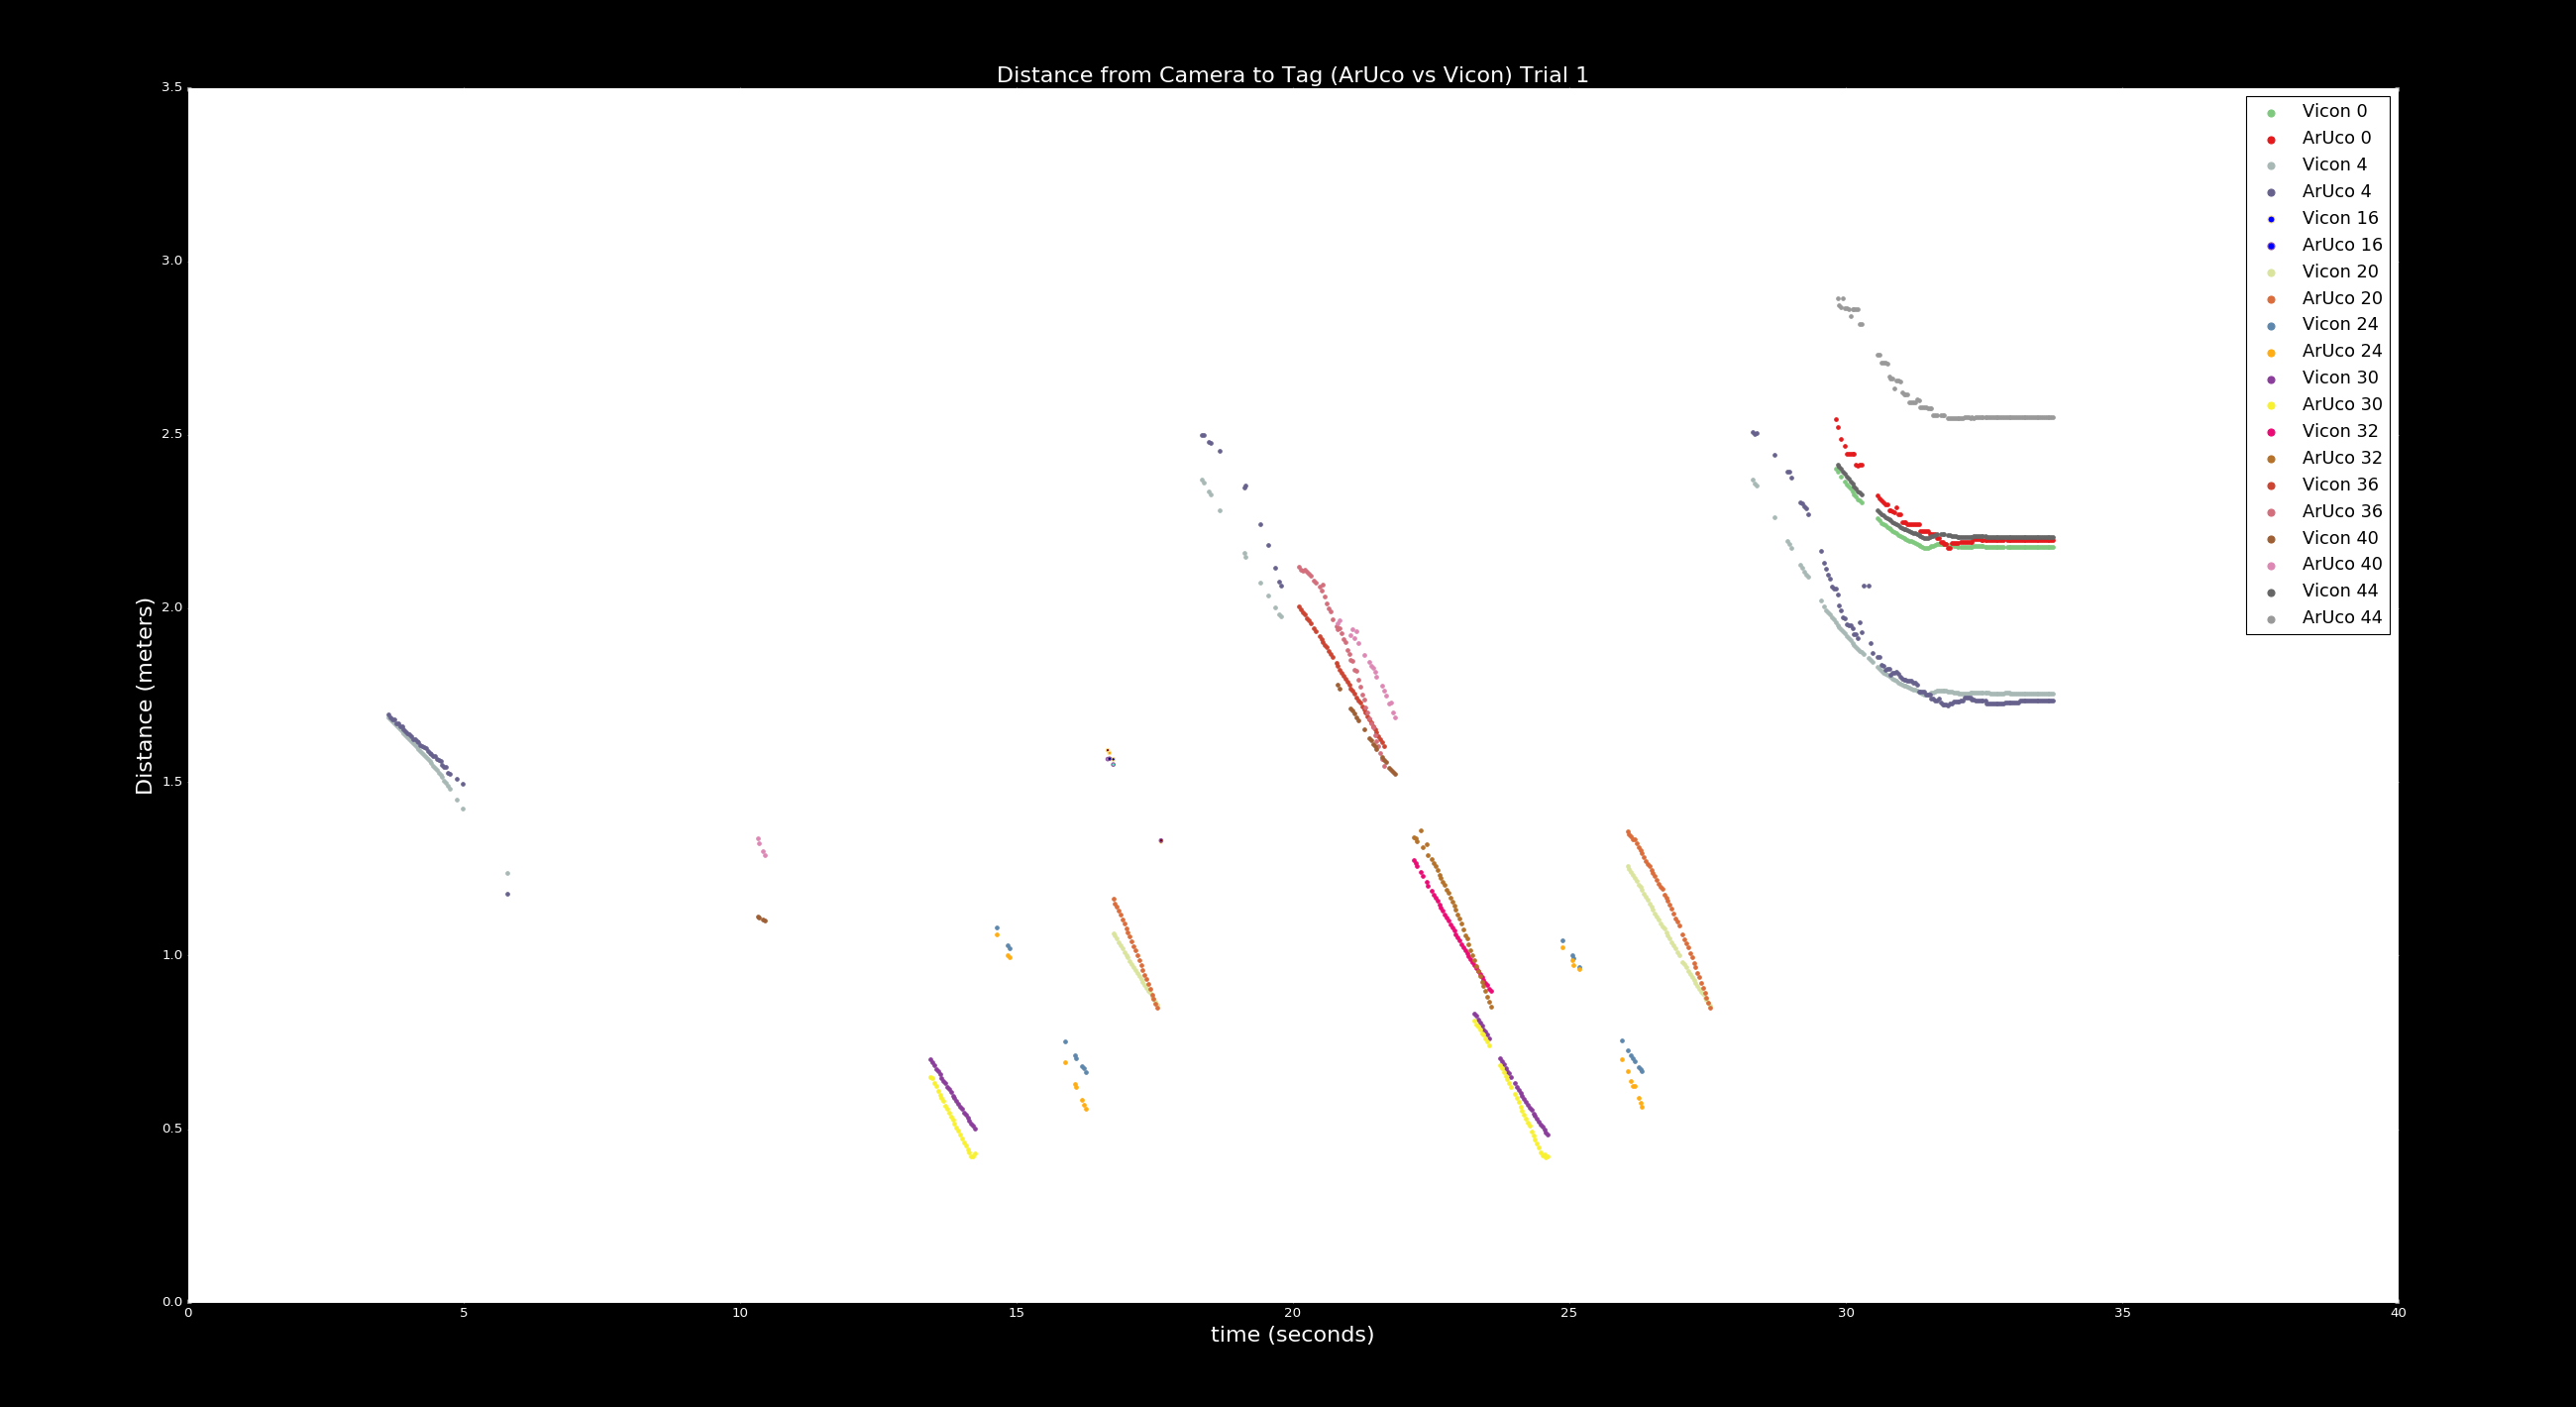
\includegraphics[width=0.98\linewidth]{./images/aruco_cam_to_tag_trial_1_3_17.png}
      \caption{One trial comparing motion capture to the output of ArUco estimte pose.}
      \label{fig:aruco_trialone_dist_comparison}
    \end{figure}

    The table below summarizes the statistics for several trials using the motion capture studio and a Kobuki Turtlebot2 mobile platform.

    \begin{table}[H]
      \centering
      \begin{tabular}{|c|c|c|c|c|} \hline
        Trial Number & Mean Error (m) & ST DEV (m) & 95th Percentile (m) & 5th Percentile (m) \\ \hline
        1 & 0.111 & 0.144 & 0.523 & 0.007 \\ \hline
        2 & 0.112 & 0.128 & 0.376 & 0.008 \\ \hline
      \end{tabular}
      \caption{Comparing pose estimates from two circular trajectories under motion capture.}
      \label{table:aruco_accuracy}
    \end{table}

    Anaysis of trials conducted under the motion capture studio revealed that ArUco pose estimates can be a reliable source of global position updates to within \SI{12}{\centi\meter} error on average. One to two outlier tags are present in each trial; it is recommended to use multiple tags when relying on ArUco for an absolute pose estimate. Although outliers can result in larger errors, on average, ArUco pose estimates are approximately within the \SI{10}{\centi\meter} error range determined suitable for localization.

	\subsection{Our Experiences with Building MarkerMaps} \label{section:building_maps_sucks}
    A protocol for generating Marker Maps with low transformation errors is necessary to successfully obtain pose estimates. To demonstrate that this process is nontrivial, two marker maps are show. The left map was generated using a video collected from a robot a testing involving teleoperation. The marker map on the right was generated using the experimentally derived protocol. Poses of tags are shown in blue; camera poses are shown in green. The origin is marked red. For both trials, the same camera parameters, tag sizes, and dictionary files were used.

    \begin{figure}[H]
      \centering
      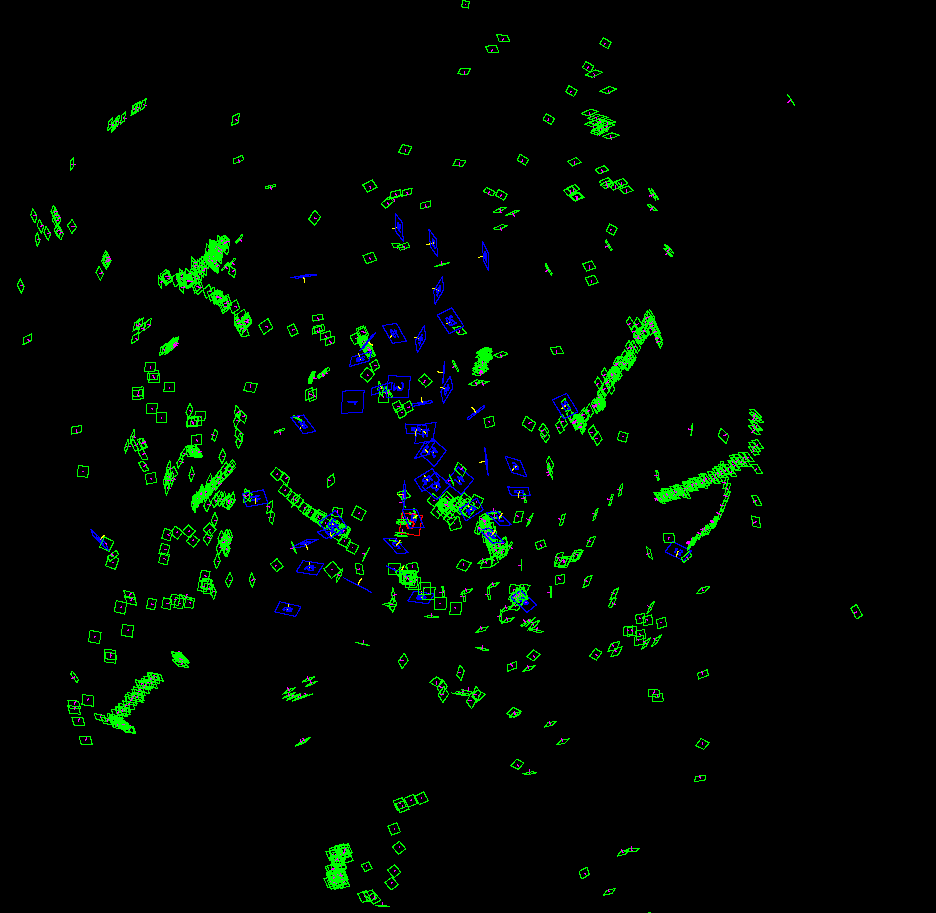
\includegraphics[width=0.49\linewidth]{./images/marker_mapper_example_bad.png}
      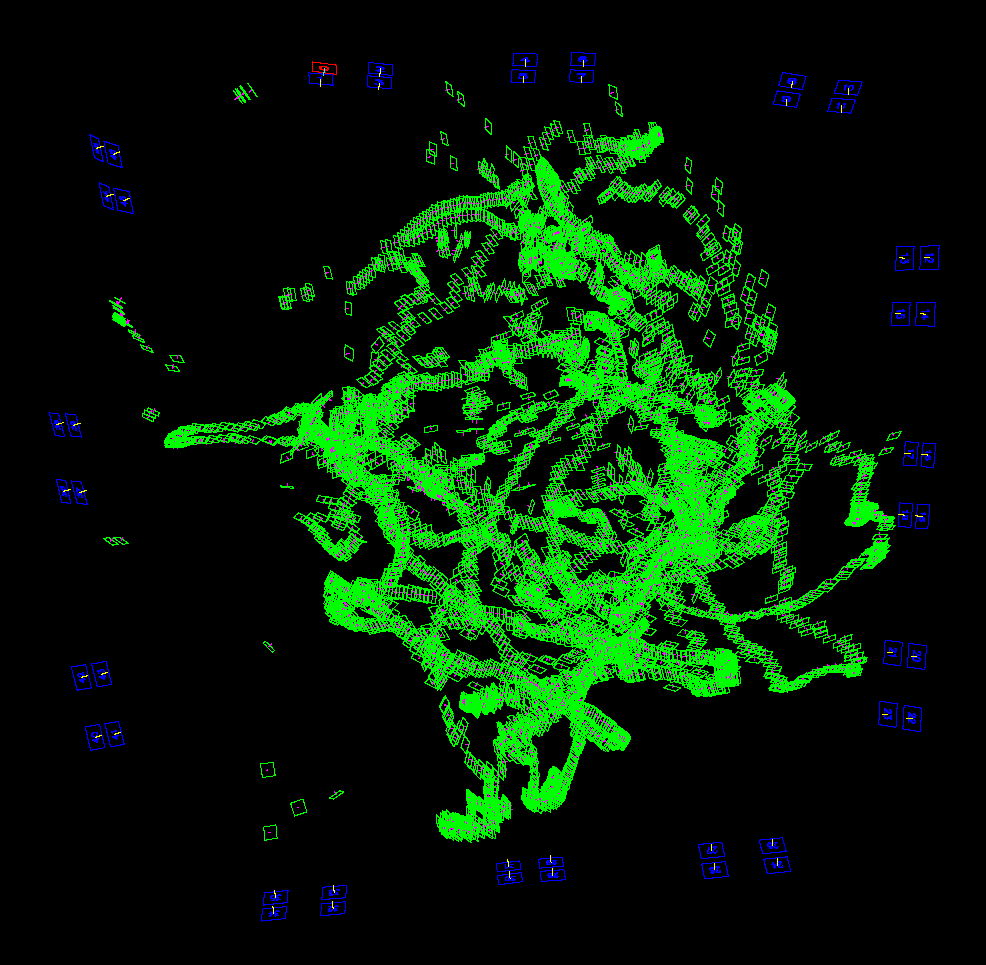
\includegraphics[width=0.49\linewidth]{./images/marker_mapper_good_ps3_3_17.png}
      \caption{Comparison of two Marker Maps generated by a robot teleop trajectory and a human walking.}
      \label{fig:marker_mapper_comparison}
    \end{figure}

    To generate marker maps that are accurate to within \SI{11}{\centi\meter}, tags must be placed maximally 4 feet apart, camera frames be collected containing many instances of transforms between tags, and frames must be stable. High tag density is important to ensure that frames contain many tags (transform data is collected) and to improve local optimization techniques that rely on detections with low reprojection errors (more tags results in more chances of detections with low reprojection errors, necessary for generating good pose quivers)\cite{munoz-salinas_rafael_mapping_2016}. In our experiments, a sufficient density comprised 3 to 4 feet of spacing between tags. To further improve the optimization process, collecting redundant camera frames is useful. Scanning small portions of the map at a time ensures that one continuous pose graph is built. Multiple discontinuous graphs cause the optimization process to fail and prevent generation of the map. ArUco tag detection and pose estimation fail to process blurred frames. Camera stability is crutial to collecting a set of frames result in low reprojection error on detection of tag corners. A clear, stable image results in lower reprojection errors when the pose of the tag is calculated. In practice, the angle of the plane corresponding to the camera's Z axis (pointing out from the camera) is ambiguous; therefore, the Planar Pose Estimation algorimth in ArUco outputs two solutions with corresponding reprojection errors. The solution with the lower error is likely the correct one, and solutions with reprojections errors that are too similar are discarded before the optimization process\cite{munoz-salinas_rafael_mapping_2016}. Therefore, it is necessary to collect sharp frames. In experimentation, cameras with a high framerate outperformed lower framerate cameras.

	\subsection{Erroneous detections with ArUco}

    Marker Maps must comprise fiducial markers from known ``dictionaries'' or binary encodings. Examples of a several dictionaries are shown below. Dictionary selection is important because it allows users to optimize their Marker Maps. Users can choose dictionaries with different numbers of tags, marker (square) sizes, and inter-marker distances. Inter-marker distances are determined by the number of tags in the dictionary (high distances correspond to low numbers of tags). High inter-marker distances make detection more robust. Tags are defined by a list of bytes which determine the color of squares. Dictionaries can be further optimized by setting the ``maxCorrectionBits'' parameter experimentally to reduce false positives\cite{open_source_computer_vision_detection_2015}.

    Throughout our experiments with ArUco tags, we accumulated several examples of detections that were erroneous in some form or another. First, we present examples of tags whose ID is misdetected (Figure \ref{fig:misdetected_tags}). In all these cases the incorrectly detected ID was 2, but there is no evidence that this is an issue just with tag 2 specifically.

    \begin{figure}[H]
      \centering
      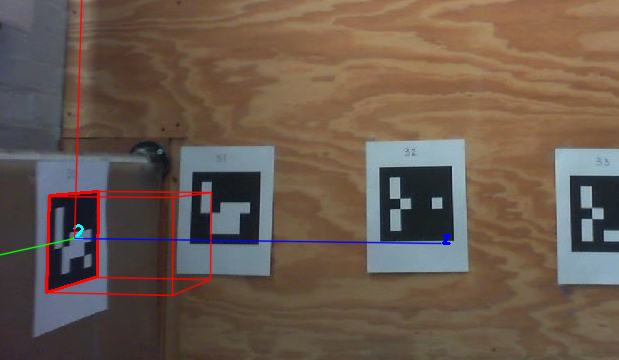
\includegraphics[width=0.49\linewidth]{./images/misidentified_tag_1.png}
      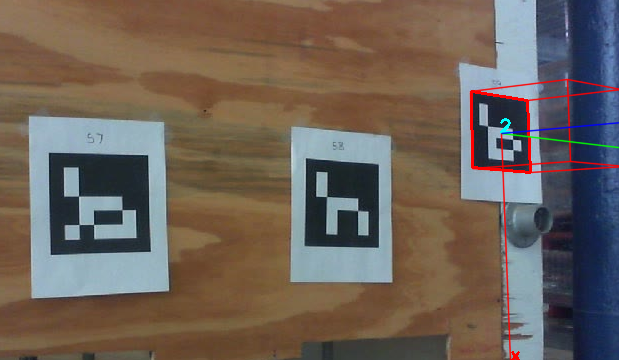
\includegraphics[width=0.49\linewidth]{./images/misidentified_tag_2.png}
      \includegraphics[width=0.49\linewidth]{./images/misidentified_tag_3.png}
      \includegraphics[width=0.49\linewidth]{./images/misidentified_tag_4.png}
      \caption{Tags that were detected, but with the wrong IDs}
      \label{fig:misdetected_tags}
    \end{figure}

    We also report how a poor camera calibration file and cause inaccuracies in the estimated poses of tags. In Figure \ref{fig:bad_tag_pose}, the tag's ID is identified correctly, but it's orientation is incorrect.

    \begin{figure}[H]
      \centering
      \includegraphics[width=1\linewidth]{./images/bad_tag_pose_1.png}
      \caption{Example of poor camera calibration file causing skewed pose estimate.}
      \label{fig:bad_tag_pose}
    \end{figure}

	\subsection{Latency over the Robot Network}

		It is important that all of our sensor data be time stamped so we can account for latency in our state estimation. The data collected on the NavX is time stamped on the NavX, and the encoder data is stamped when it is read on the RoboRIO. This time stamped data is sent to the TK1 over UDP. UDP was chosen because it was the easiest method with satisfactory speed. To test this, we wrote a simple program that sends 96 bytes, an upper bound on the size of all our stamped sensor data, of UDP data between the RoboRIO and the TK1. We recorded the round trip time of these packets, which can be seen in Figure \ref{fig:udp_timing}. The round-trip latency was \SI{0.5}{\milli\second} on average, which is much faster than any of our sensors, and therefore is fast enough for us to transmit and process the data before new data arrives.

		\begin{figure}[H]
			\centering
			\includegraphics[width=0.7\linewidth]{./images/rio_tk1_udp_latency_timeseries.png}
			\caption{RTT of UDP packets between the RoboRIO and the TK1 over the robot's wired network.}
			\label{fig:udp_timing}
		\end{figure}

		Another important problem is time synchronization. The time stamps on all the data must be in reference to some common time source. To achieve this effect, we use Christian's Algorithm \cite{cristian_probabilistic_1989}. Specifically, we send a packet stamped with the current time on the RoboRIO to the TK1, the TK1 adds its own time stamp and responses, the and RoboRIO then add half the round trip time to the time sent by the TK1. This allows the sensor data sent from the RoboRIO to be synchronized with the clock on the TK1.




\section{A Dataset for Robot Localization} \label{section:dataset}

  We have collected a corpus of sensor data and ground-truth position labels from many of the tests performed for this MQP. In this section, we document the different collections of data and indicate how it could be used in the development of localization systems. Note that any details not listed here, such as exact column headings or detailed descriptions of how the data was collected, are contained in the \texttt{README.md} files of each respective dataset.

  \begin{table}[H]
    \centering
    \begin{tabular}{|l|l|} \hline
      dataset name (url) & brief description \\ \hline
      \href{https://users.wpi.edu/~pdmitrano/phil-datasets/turtlebot_mocap_complete.tar.gz}{\texttt{turtlebot\_complete}} & full sensor data with maps in ground truth\\ \hline
      \href{https://users.wpi.edu/~pdmitrano/phil-datasets/field_data_1.tar.gz}{\texttt{field\_data\_1}} & realistic driving data and multiple video stream \\ \hline
      \href{https://users.wpi.edu/~pdmitrano/phil-datasets/field_data_2.tar.gz}{\texttt{field\_data\_2}} & realistic driving data and multiple video stream \\ \hline
      \href{https://users.wpi.edu/~pdmitrano/phil-datasets/field_data_3.tar.gz}{\texttt{field\_data\_3}} & realistic driving data and multiple video stream \\ \hline
      \href{https://users.wpi.edu/~pdmitrano/phil-datasets/imu_calibration.tar.gz}{\texttt{imu\_calibration}} & Raw accelerometer and gyroscope readings \\ \hline
      \href{https://users.wpi.edu/~pdmitrano/phil-datasets/markermaps.tar.gz}{\texttt{markermaps}} & Marker maps build in motion capture and on an FRC field \\ \hline
    \end{tabular}
    \label{table:datasets}
  \end{table}

  The dataset \texttt{turtlebot\_complete} consists of 9 trials of a Turtlebot 2 driving under teleoperated control with tags placed in a perimeter around the motion capture area. For each trial, we have recordings of camera frames at two different settings (480p 60fps and 1080p 30fps), encoder ticks from the kobuki base, and accelerometer, gyroscope, fused yaw, and temperature data from the RoboRIO. We have corresponding ground-truth labels for both the position of the robot, and the tags placed around the environment. We also provide three different maps built with the tags. One map was built with a C920, and the other two were built with a PS3Eye camera. The maps are quite different, despite being built back-to-back with the same general procedure. This demonstrates that the quality of the map produced is highly dependant on the which tags were seem with which other tags. In our experience, building markermaps is a highly unreliable process (see \ref{section:building_maps_sucks}), so we include multiple maps to demonstrate this.

  The \texttt{field\_data\_2} and \texttt{field\_data\_3} datasets were collected Team 126's practice FRC field (Sponsored by Nypro Inc.). In each of those two datasets, we ran one trial called \texttt{auto} where the robot drive in a series of concentric circles with static intervals in between, as well as a series called \texttt{drive} of realistic FRC driving patterns for about one minute. To simulate FRC driving patterns, we drove the robot to and from mock ``Switch'', ``Scale'', and ``Feeder Station'' field elements (from the 2018 FRC game). The driver during these tests participated in FRC for two years, and so we claim from experience that these driving patterns are realistic. During both the \texttt{auto} and \texttt{drive} trials, we recorded time stamped image frames from three camera as different resolutions and frame rates. Additionally, we recorded acceleration, rotational velocity, yaw angle, and motor set values from the NavX IMU plus encoder data from the drive wheels.

  In the \texttt{imu\_calibration} dataset, we include 6 logs of raw accelerometer and gyroscope readings taking according to our calibration procedure (see \ref{section:imu_calibration}, also \cite{tedaldi_robust_2014}). Generally, each of these logs contains a series of sample taken at a fixed rate consisting of a number of static intervals with dynamic motion between them. In fact, you can reproduce the exact calibration values we use in our sample implementation using the \texttt{imu\_calibration\_data\_1\_28\_final.csv} file as input to the \texttt{python/recorded\_data\_processing/imu\_calibration.py} script. In addition, we also include 5 logs of pure stationary IMU data. This can be useful for measuring bias and testing basic data processing.

  We also release a set of example markermaps we have built in the \texttt{markermaps} dataset. Unfortunately, we do not have the accompanying video used the build that map. Nonetheless, we hope that these maps can be used by others to see how the map files are structured and to test the API the uses them. This dataset consists of 11 marker maps. 10 of these were built in our the motion capture arena, of which three have ground-truth tag pose information from the motion capture. Our last markermap was built at the Nypro test FRC field (used by FRC Team 261).


  \subsection{Provided Tools} \label{section:tools}

    In order to conduct analysis on all the above mentioned datasets, we wrote several command line python scripts to load, process, and visualize our data. As mentioned in Appendix \ref{appendix:code}, all our code is available on Github, but we briefly mention the different functions which our tools provide.

    First, we point out that MarkerMapper and ArUco contain a collection of incredibly useful command line programs for creating calibration files, generating marker maps, stepping through videos and viewing detections, and even localizing to makermaps. In addition, we provide a tool that will detect markers in a video recorded on the robot and match those detections with the time stamps which were collected in unison with the video frames. This allows one to know not just the location of the detected tag, but the time stamp at which the detection occurred. We also provide a program for generating custom ArUco dictionaries. In our experiments with MarkerMapper, we found it necessary to use custom dictionaries to restrict the tags which could be detected. This helped mitigate false tag detections, and so we provide this tool for others to use. Further, we include a script that computes statistics about the frames per second given as input a file containing timestamps of frames.

    We include python code which can process with CSV files exported motion capture into useful NumPy data structures \cite{jones_scipy.org_2001}.

    Perhaps most importantly, we also provide the python script we used for IMU calibration. This serves as a reference implementation of the procedure described in \cite{tedaldi_robust_2014}, and can be used for any project requiring IMU calibration.




\section{Sample Implementation} \label{section:specs}

  In order to evaluate the theory and research presented above, we built a complete localization system using a RoboRIO (courtsey of our sponsor National Instruments), an FRC Chassis (courtesy of AndyMark), and NavX-MXP IMU (courtesy of Kauai Labs), encoders, and a PS3Eye webcam. In this section, we describe the details of this system and explain the lessons learned from implementing and testing the platform.

  \subsection{Sensing Techniques Used}\label{section:techniques_used}

    Our simple implementation includes three of the five proposed localization techniques (see \Newnameref{section:proposed_techniques}). We limited ourselves to only three methods because of time constraints. We used an IMU, Drive wheel encoders, and a Camera for ArUco tags. We chose this subset because they were easy to implement, because they are the most accessible to an FRC team, and because they included both local and global position estimates. We have found examples in the literature of each of these techniques being used successfully, and in some cases our experiments we have verified that they satisfy our criteria for accuracy, precision, update rate, and accessibility criteria. Therefore, chooses these three techniques was justified.

	\subsection{Robot Hardware}

    A picture of the robot we built can be seen in Figure \ref{fig:mocap_robot}. This robot consists of an AndyMark chassis (am-2240) with Toughbox gearboxes (similar to am-0977), and two sets of 6in wheels. The back wheels have more traction than the front, which means the robot will slip. This provides interesting and challenging dynamics--a simple Dubin's car or differential drive model is inaccurate. From our experience in FRC, we know off-center turning is a common feature of FRC robots. We use two \href{https://www.digikey.com/product-detail/en/grayhill-inc/63R256/GH3070-ND/304479}{Greyhill 63R256} encoders with 256 pulses per revolution. Because the gear ratio of our gearboxes is unknown, it was simpler to directly measure distance per pulse, which we found to be \SI{0.000375}{\meter} per pulse.

    \begin{figure}[H]
      \centering
      \includegraphics[width=1\linewidth]{./images/mocap_robot.jpg}
      \caption{An FRC-style robot we used in many of our tests}
      \label{fig:mocap_robot}
    \end{figure}

    In addition to the RoboRIO, we use a Raspberry Pi 3 a our co-processor. We use the Raspberry Pi for image processing (see \ref{section:profiling_opencv}), and connect a PS3Eye camera capable of 460x480 video at 60fps. The main program which accumulates sensor data and computes position also runs on the Raspberry Pi.

	\subsection{Kalman Filtering}

    In order to fuse measurements from our three sensors, we used an extended Kalman filter. Based on our literature review, we found a common EKF formulation for robot localization was to use the measured wheel speeds as the control input $u$, and other sensors as measurements $z$ \cite{thrun_probabilistic_2005}. We chose an extended Kalman filter because it has been shown many times to be effective at fusing encoder and IMU data \cite{marin_multi_2013}\cite{teslic_ekf-based_2011}\cite{thrun_probabilistic_2005}. In our sample implementation, we have three measurement sources: Acceleration from the NavX, yaw from the NavX, and position from the camera. We also considered an alternate formulations, where the accelerometer was treated as the control input, and where the voltages or current to the motors were the control inputs. We ultimately settled on using encoders because we found it was more common. Additionally, if current were used we would have needed to purchase additional FRC control system components. Exploring the trade-offs between different EKF formulations, or even different sensor fusion approaches, would be a worthy goal for future MQPs. We show the full form of the prediction step of our EKF in Equation \ref{eq:ekf_prediction}. We denote the value of a state variable at time $t$ with an underscore. The hat symbol ($\hat{x}$) indicates that it is an intermediate predicted state variable. Note we also assume a constant time interval, $\Delta t$. The linear velocity of the wheels, $v_l$ and $v_r$ are our control input. Note we do not need to model rotational acceleration, because we can directly measure the yaw angle ($\theta$) and we can predict the rotational velocity directly from our wheel speeds. The $\alpha$ parameter is a slip coefficient that must be greater than 1 \cite{yu_dynamic_2011}. We use $W$ to represent that track width of the robot.

    \begin{align} \label{eq:ekf_prediction}
      \begin{split}
        v &= \frac{v_l + v_r}{2} \\
        \hat{x}_{t+1} &= x_t + \dot{x}_t\Delta t + \tfrac{1}{2}\ddot{x}_t\Delta t^2 \\
        \hat{y}_{t+1} &= y_t + \dot{y}_t\Delta t + \tfrac{1}{2}\ddot{y}_t\Delta t^2 \\
        \hat{\theta}_{t+1} &= \theta_t + \dot{\theta}_t\Delta t \\
        \hat{\dot{x}}_{t+1} &= v\cos(\theta_t) \\
        \hat{\dot{y}}_{t+1} &= v\sin(\theta_t) \\
        \hat{\dot{\theta}}_{t+1} &= \frac{v_r - v_l}{\alpha W} \\
        \hat{\ddot{x}}_{t+1} &=  \ddot{x}_{t} \\
        \hat{\ddot{y}}_{t+1} &=  \ddot{y}_{t} \\
        \hat{\ddot{\theta}}_{t+1} &= 0 \\
      \end{split}
    \end{align}

    Because the EKF requires a linearized version of the above state-space equations, we must provide a Jacobian matrix. This matrix contains the partial derivatives of each state variable update equation with respect to each state variable. The shape is therefore a square matrix the same size as the state space, which in our formulation means 9x9. The full analytic Jacobian is shown in Equation \ref{eq:ekf_jacobian}.

    \begin{equation} \label{eq:ekf_jacobian}
      \begin{bmatrix}
        1 & 0 & 0 & \Delta t & 0 & 0 & 0.5\Delta t^2 & 0 & 0 \\
        0 & 1 & 0 & 0 & \Delta t & 0 & 0 & 0.5\Delta t^2 & 0 \\
        0 & 0 & 1 & 0 & 0 & \Delta t & 0 & 0 & 0 \\
        0 & 0 & -v\sin(\theta_t) & 0 & 0 & 0 & 0 & 0 & 0 \\
        0 & 0 & v\cos(\theta_t) & 0 & 0 & 0 & 0 & 0 & 0 \\
        0 & 0 & 0 & 0 & 0 & 0 & 0 & 0 & 0 \\
        0 & 0 & 0 & 0 & 0 & 0 & 1 & 0 & 0 \\
        0 & 0 & 0 & 0 & 0 & 0 & 0 & 1 & 0 \\
        0 & 0 & 0 & 0 & 0 & 0 & 0 & 0 & 0 \\
      \end{bmatrix}
    \end{equation}

    The next step is to describe the measurement updates. The requirement here is to define a function that takes in the current state prediction and outputs a predicted measurement vector. Conveniently, although importantly not required by the EKF, all of our measurement updates are simple linear functions, and therefore we write them as matrix multiplications between the state column vectors $\hat{x}$ and some matrix $H$. Note in this context $\hat{x}$ is the entire 9x1 state vector, not just the $x$ component of the state. In our sample implementation, we have three H matrices: $H_{\text{acc}}$, $H_{\text{yaw}}$, $H_{\text{camera}}$. They are shown below in Equations \ref{eq:H_acc}, \ref{eq:H_yaw}, and \ref{eq:H_camera}. These matrices simply contain $1$'s because the measurements are exactly the same as the state variables, due to the pre-processing of the measurements. We will now describe these required pre-processing steps.

    \begin{equation} \label{eq:H_acc}
      H_{\text{acc}} =
      \begin{bmatrix}
        0 & 0 & 0 & 0 & 0 & 0 & 1 & 0 & 0 \\
        0 & 0 & 0 & 0 & 0 & 0 & 0 & 1 & 0 \\
      \end{bmatrix}
    \end{equation}

    \begin{equation} \label{eq:H_yaw}
      H_{\text{yaw}} =
      \begin{bmatrix}
        0 & 0 & 1 & 0 & 0 & 0 & 0 & 0 & 0 \\
      \end{bmatrix}
    \end{equation}

    \begin{equation} \label{eq:H_camera}
      H_{\text{camera}} =
      \begin{bmatrix}
        1 & 0 & 0 & 0 & 0 & 0 & 0 & 0 & 0 \\
        0 & 1 & 0 & 0 & 0 & 0 & 0 & 0 & 0 \\
        0 & 0 & 1 & 0 & 0 & 0 & 0 & 0 & 0 \\
      \end{bmatrix}
    \end{equation}

    \subsubsection{Encoder Pre-Processing}

      Because the encoders technically only measure pulses, we most convert this into linear speed. The step of converting ticks to a linear elocity of radians per second is performed on the RoboRIO in WPILib. We provide in our code the conversion from ticks to meters, and the WPILib Encoder class provides the \texttt{GetRate()} method, which returns the linear velocity of the wheels.

    \subsubsection{Accelerometer Pre-Processing}

      Like with the encoders, the accelerometer does not directly measure what we need for our Kalman filter. We apply calibration, base frame rotation, and zero velocity updates to this data before passing it to the EKF. These methods were explored in detail in sections \ref{section:imu_calibration} and \ref{section:drift_bias}. We apply the static detector described in these sections to a window of the last $80$ samples, and use the detected static intervals to compute our current bias estimates and perform zero velocity updates.

    \subsubsection{Camera Pre-Processing}

      First, we only consider frames where valid pose estimates are return from MarkerMapper. In those frames where a pose estimate is made, we may choose to transform that pose estimate into a frame other than the MarkerMapper frame. In the MarkerMapper frame, everything is relative to the origin tag, which is usually tag 0. Unless that origin tag is placed on the floor facing up where the desired origin is, you may want to rotate the pose measurements from MarkerMapper before feeding them into the EKF. We omit this in our implementation for simplicity, and instead assume that tag 0 is placed on the floor at the desired origin.

  \subsection{Software Design}

    There are two software components of our sample implementation. First, there is a C++ library that is cross-compiled for the RoboRIO that FRC teams will use in their robot projects. We use the standard Eclipse-based C++ development environment and write our robot projects the same way an FRC team would. Teams are expected to call two or three simple functions in their robot program, which gives us everything we need to log sensor data and send it to the co-processor. Because of this minimal API, we require very few changes to robot programs in order to get localization. This would make it approachable for teams and encourage them to try localization. This library is called \texttt{phil\_rio} and is built and installed to ones \texttt{\textasciitilde/wpilib} directory.

    The second software component is a C++ program running on the co-processor. This program reads the camera data from a CSCore camera stream, serves an annotated version of the camera stream, receives the IMU and encoder data from the RoboRIO, computes the position of the robot, and reports this position over network tables. See \ref{fig:software_diagram} for a diagram of this system.

    \begin{figure}[H]
      \centering
      \includegraphics[width=1\linewidth]{./images/MQP_System_Chart.png}
      \caption{A diagram of our software}
      \label{fig:software_diagram}
    \end{figure}




\section{Conclusion} \label{section:conclusion}

  This MQP conducted a thorough survey of localization techniques and isolated 5 techniques which are most promising for localization in high-speed, cluttered, multi-robot environments, such as FRC. We conducted a series of experiments to characterize our sensors and determine how accurate each method could be. We conclude that naive double integration of accelerometer data is inaccurate, but that applying calibration and zero velocity updates improve the accuracy. We find that a 480p60 camera is sufficient for detecting tags extremely on average ever \SI{33}{\milli\second} even with a 6ft spacing between tags. However, we show that a 6ft spacing is too sparse to build accurate MarkerMaps, and that building MarkerMaps in general is tricky. We offer suggestions on how to improve the likelihood of building an accurate map, and provide accuracy measures on maps built in a motion capture studio. Furthermore, we offer a sample implementation using an IMU, encoders, and a camera. This sample implementation provide a detailed example of how to filter all of these sensors together in a principled way, and it allowed us to explore some of the challenges of implementing a real localization system on a real robot. Due to time constraints, we were unable to benchmark the accuracy of our system, but we were able to demonstrate all of the sensor systems being collected, transported, and processed by the extended Kalman filter.



\section{Future Work} \label{section:future_work}

  The goals of our MQP were to develop a solid understanding of a breadth of localization techniques, and to rigorously study their characteristics and performance. Therefore, there remains a lot of work to be done on turning this into a packaged system usable by someone other than its authors. We see a great opportunity for a future MQP to use our experiments, datasets, and sample code to build a real localization system for FRC that meets all the criteria outlined in Section \ref{section:defining_success}. The first steps for such a project would be to finish the accuracy benchmarking of our sample implementation and then iterate on the implementation details until the system meets our design criteria.

  Alternatively, there is much more research to be done on beacons and optical flow. From the few experiments we did with these techniques and from all our background research, we believe these techniques are capable of contributing to the accuracy of a complete localization system. One could explore replacing ArUco and MarkerMapper with Beacons, or augmenting forward kinematics form encoders with optical flow. Beacons in particular are a very promising technique, although as we discovered in our early experiments, making beacons successful requires a lot of analog or digital signals processing knowledge. A good first step for these additional techniques could be to develop an algorithm for accurately detecting the arrival time of an ultrasonic chirp in the presence of Doppler shift. One could also start by exploring algorithms to turn optical flow vector fields into an estimate of the motion of the camera.




\section{Acknowledgements}

  We thank our advisors, Bradley Miller and William Michalson for their guidance. We also thank our sponsors, National Instruments, AndyMark, and Kauai Labs for their generous donation of hardware. We'd like to thank Scott Libert and Eric Peters for their advice. Finally, we thank FRC Team 261 Gael Force for letting us use their practice FRC field.

  \begin{figure}[H]
    \centering
    \includegraphics[width=0.30\linewidth]{./images/ni_logo_2c.png}
    \hspace*{0.1in}
    \includegraphics[width=0.25\linewidth]{./images/Logo_Type_KauaiLabs_BuildBetterRobots_TrademarkSmaller.png}
    \hspace*{0.1in}
    \includegraphics[width=0.30\linewidth]{./images/AndyMark_MedWeb.jpg}
    \caption*{}
    \label{fig:sponsors}
  \end{figure}

\bibliographystyle{plain}
\bibliography{phil-mqp}


\section{Appendices}

  \subsection{Ultrasonic Radio Beacons Bill of Materials} \label{appendix:beacon_bom}

    \begin{table}[H]
      \centering
      \begin{tabular}{|c|c|c|c|} \hline
        Item & Quantity & Cost & Extended Cost \\ \hline
        PSoc 5LP & 8 & \$10.00 & \$80.00 \\ \hline
        RF Tx/Rx Pair & 8 & \$1.68 & \$13.44 \\ \hline
        piezo speaker & 8 & \$1.65 & \$13.20 \\ \hline
        9v battery & 8 & \$1.19 & \$9.49 \\ \hline
        battery connector & 8 & \$0.54 & \$4.31 \\ \hline
        power switch & 8 & \$2.11 & \$16.88 \\ \hline
        LCD backpack & 8 & \$9.95 & \$79.60 \\ \hline
        LCD display & 8 & \$3.90 & \$31.20 \\ \hline
        passive components & 8 & \$5.00 & \$40.00 \\ \hline
        prototyping board & 8 & \$5.00 & \$40.00 \\ \hline
        TOTAL & & & \$328.12 \\ \hline
        COST PER BEACON & & & \$41.02 \\ \hline
      \end{tabular}
      \caption{Estimated Bill of Materials assuming 8 beacons.}
      \label{table:beacon_bom}
    \end{table}

  \subsection{Survey Responses}\label{appendix:survey}

    \begin{figure}[H]
      \centering
      \includegraphics[height=4.2cm]{./images/survey_angle.png}
      \includegraphics[height=4.2cm]{./images/survey_position.png}
      \includegraphics[height=4.2cm]{./images/survey_worth.png}
      \label{fig:survey_imgs}
    \end{figure}

  \subsection{Radio Time of Flight}\label{appendix:rf-rx-tx}

    \begin{table}[H]
      \begin{tabular}{|l|l|l|l|l|}
        \hline
        Measured Distance (m) & \multicolumn{3}{|l|}{Measured Total Time ($\mu$s)} & Average Delay \\
        \hline
        0.0630 & 45.44 & 42.80 & 34.48 & 40.90646 \\
        0.1425 & 52.72 & 50.48 & 52.09 & 51.76286 \\
        0.1505 & 64.16 & 63.36 & 60.24 & 62.58616 \\
        0.2210 & 40.33 & 36.79 & 36.40 & 37.83926 \\
        0.2415 & 49.52 & 45.76 & 43.92 & 46.39919 \\
        0.2460 & 47.47 & 53.84 & 44.71 & 48.67251 \\
        0.2965 & 34.36 & 34.00 & 43.76 & 37.37234 \\
        0.3085 & 79.36 & 62.16 & 59.52 & 67.01230 \\
        0.3390 & 39.92 & 57.27 & 38.96 & 45.38220 \\
        0.3770 & 41.75 & 40.75 & 45.53 & 42.67541 \\
        0.3600 & 38.40 & 38.40 & 37.68 & 38.15880 \\
        0.0070 & 35.60 & 36.08 & 34.32 & 35.33331 \\
        \hline
        \multicolumn{4}{|r|}{Average Delay ($\mu$s)} & 46.175 \\
        \hline
      \end{tabular}
      \caption{The time of flight of radio over tens of centimeters is insignificant compared to the delay within the transmitter and receiver.}
      \label{table:rf-rx-tx}
    \end{table}

  \subsection{ArUco Detection Times}\label{appendix:tag_detection}

    \begin{figure}[H]
      \centering
      \includegraphics[width=1\linewidth]{./images/detection_times_480p30.png}
    \end{figure}
    \begin{figure}[H]
      \centering
      \includegraphics[width=1\linewidth]{./images/detection_times_480p60.png}
    \end{figure}
    \begin{figure}[H]
      \centering
      \includegraphics[width=1\linewidth]{./images/detection_times_1080p15.png}
    \end{figure}

  \subsection{Code \& Dataset}\label{appendix:code}

    All of the code used in the above experiments, including the sample implementation and some of the raw sensory data (minus large video files) are available in our github repository: \url{https://github.com/PHIL-MQP/phil}. For the datasets, the urls are encoded in the table in section \ref{section:dataset}.

\end{document}
